\documentclass[12pt,twoside]{thesis92e}
\usepackage[utf8]{inputenc}
\usepackage{graphicx}
\usepackage{physics}
\usepackage{gnuplottex}
\usepackage{pgfplots}
\usepackage{pgfplotstable}
\usepackage{fancyhdr}
\usepackage{amsmath}
\usepackage{verbatim}
\usepackage{amsmath}
\usepackage{amsfonts}
\usepackage{mathtools}
\usepackage{bm}
\usepackage{mathrsfs}
\usepackage[utf8]{inputenc}
\usepackage[english]{babel}
%\usepackage[style=phys]{biblatex}
\usepackage{setspace}
\usepackage{csquotes}
\usepackage{comment}
\usepackage{booktabs} % For \toprule, \midrule and \bottomrule
\usepackage{siunitx} % Formats the units and values
\usepackage{pgfplotstable} % Generates table from .csv
\usepackage[colorlinks=false]{hyperref}
\usepackage[square, numbers]{natbib}
\usepackage[titletoc, title]{appendix}
%\newcommand{\appendixnumberline}[1]{Appendix\space}
\renewcommand\appendixtocname{Appendix}




%\bibliography{bib-refs.bib}
%\addbibresource{references.bib}
\pagestyle{fancy}
\graphicspath{{images/}}
%\usepackage[a4paper,width=150mm,top=25mm,bottom=25mm]{geometry}
%\usepackage[a4paper,width=150mm,top=25mm,bottom=25mm,bindingoffset=6mm]{geometry}
\setlength{\headheight}{15pt}
\fancyhead[]{}
\fancyhead[RO,LE]{Two Photon Processes within the Hyperfine Structure of Hydrogen}
\fancyfoot{}
\fancyfoot[LE,RO]{\thepage}
\fancyfoot[LO,CE]{Chapter \thechapter}
\fancyfoot[CO,RE]{Spencer Percy}

\title{
    {Two Photon Processes within the Hyperfine Structure of Hydrogen}\\
    {\large University of Windsor}
}    
\author{Spencer Percy }
\date{July 2018}
%\doublespacing
%\onehalfspacing
\pgfplotsset{compat=1.15}

%\sisetup{
%  round-mode          = places, % Rounds numbers
%  round-precision     = 3, % to 2 places
%  scientific-notation = true
%}

\begin{document}
\prepages

\begin{titlepage}
    \begin{center}
        \vspace*{1cm}
        \Huge
        \textbf{Two Photon Processes within the Hyperfine Structure of Hydrogen}
        
        \vspace{0.5cm}
        \large
              \textbf{by}

        
        \vspace{0.5cm}
        \large
        \textbf{Spencer Percy}
        
        \vfill
        
        A Thesis\\
        Submitted to the Faculty of Graduate Studies\\
        through the Department of Physics in Partial Fulfillment\\
        of the Requirements for the Degree of Master of Science at the\\
        University of Windsor
        
        \vspace{0.8cm}
        

        Windsor, Ontario, Canada\\
        \textcopyright 2018 Spencer Percy
        
    \end{center}
\end{titlepage}
\begin{approval}
\begin{center}
	\textbf{ \large Two Photon Processes in the Hyperfine Structure of Hydrogen} \\
	by \\
	Spencer Percy \\





APPROVED BY:







~\\ \rule{10 cm}{.5pt} \\
M. Monfared \\
Department of Mathematics and Statistics


~\\ \rule{10 cm}{.5pt} \\
E.H. Kim \\
Department of Physics




~\\ \rule{10 cm}{.5pt} \\
G.W.F. Drake, Advisor \\
Department of Physics







\end{center}
\begin{flushright}
	December 10, 2018
\end{flushright}



\end{approval}


\addtocounter{page}{2}

%\begin{center}
%    \begin{LARGE}
%    \textbf{Author’s Declaration of Originality}
%    \end{LARGE}
%  \end{center}
\chapter*{Author's Declaration of Originality}
\addcontentsline{toc}{chapter}{Author’s Declaration of Originality}
I hereby certify that I am the sole author of this thesis and that no part of this thesis has been published or submitted for publication.

I certify that, to the best of my knowledge, my thesis does not infringe upon anyone’s copyright nor violate any proprietary rights and that any ideas, techniques, quotations, or any other material from the work of other people included in my thesis, published or otherwise, are fully acknowledged in accordance with the standard referencing practices. Furthermore, to the extent that I have included copyrighted material that surpasses the bounds of fair dealing within the meaning of the Canada Copyright Act, I certify that I have obtained a written permission from the copyright owner(s) to include such material(s) in my thesis and have included copies of such copyright clearances to my appendix. 
 
I declare that this is a true copy of my thesis, including any final revisions, as approved by my thesis committee and the Graduate Studies office, and that this thesis has not been submitted for a higher degree to any other University or Institution.

\chapter*{Abstract}
\addcontentsline{toc}{chapter}{Abstract}\thispagestyle{plain}
%\begin{center}
%%    \Large
%    \textbf{Abstract}
%\end{center}
% We have shown that the the transition between the hyperfine energy levels of hydrogen can be connected by means of a two-photon electric dipole process. From this we have calculated the two-photon decay rate of the hyperfine levels in the ground state of hydrogen and shown that it does not need to be considered as a significant correction to recombination. From this we have also calculated the Einstein B coefficient for the absorption rate and applied to to a few scenarios to see if it would make a significant impact to astrophysics. We have also taken these energy levels and treated them as a Raman scattering process and calculated the relevant cross section.

%We have extended these calculations to other hydrogenic ions. We have made an approximation to the hyperfine splitting in the ground state of heavier ions and used this to calculate the decay rate, absorption coefficient and Raman scattering cross section for all stable nuclear spin $1/2$ isotopes from helium to bismuth.

The hyperfine levels for the ground state of hydrogen are normally connected by magnetic dipole transitions.  However, for astrophysical applications, it may be that two-photon electric dipole processes are also important over cosmological distances. This thesis sets up a general mathematical formalism for the calculation of two-photon processes within the hyperfine structure of an atom with spin $1/2$, and applies it to the ground state of hydrogen. Rates are calculated for both spontaneous emission and absorption of radiation. Due to an extraordinary degree of cancellation in the matrix elements, the rates turn out to be too small to have a significant impact on astrophysical processes involving the absorption and emission of radiation. The results are nevertheless important in reducing the uncertainty due to possible contributions from these processes.  Other two-photon processes involving Raman scattering are also considered and the relevant cross sections calculated. The calculations of the decay rate, absorption coefficient and Raman scattering cross section are extended to heavier hydrogenic ions as a function of the nuclear charge $Z$, using an approximate interpolation formula for the hyperfine splitting in the ground state. Results are presented for the hydrogenlike ions from He$^+$ to Pb$^{81+}$. Modifications for the case of isotopes with a nuclear spin greater than $1/2$ are briefly considered. 


\chapter*{Dedication}
\addcontentsline{toc}{chapter}{Dedication}
To Erica, I couldn't have done this without you.


\chapter*{Acknowledgements}
\addcontentsline{toc}{chapter}{Acknowledgements}I'd like to thank my girlfriend Erica Dionisi for constantly helping me to suppress my imposter syndrome and always being in my corner. Daniel Venn for being the most consistent brotégé I've ever had. Maha Sami for keeping the investigation into the identity of her husband alive. Aaron Bondy for his vast knowledge of Drew Dilkins. Kimberly Lefebvre for constantly listening to me complain. Joshuah Trocchi for being a friendly face while he squats in our office. Peipei Zhang for all the delicious moon cakes. A special thank you goes to the crew of The White Raven for saving the world from the Dread Captain Tiberius Flint

None of this work could have be possible without the guidance and knowledge of my supervisor Dr. Gordon Drake. I would like to thank him for his constant tutelage in helping me understand the depth of the physical world.

\tableofcontents

\clearpage\addcontentsline{toc}{chapter}{List of Figures}\listoffigures
\clearpage\addcontentsline{toc}{chapter}{List of Tables}\listoftables

\mainbody
\pagestyle{fancy}
\chapter{Introduction}
The purpose of this work is to take the well known hyperfine splitting in the ground state of hydrogen, and investigate two-photon transitions from the lower hyperfine level to the upper hyperfine level to see if the resulting absorption coefficient is a significant correction to astrophysical and cosmological phenomena. We are interested to see if the absorption coefficient is significant enough that it will provide a significant correction to light that is observed from distant stars. As the light travels through space it is absorbed by the hydrogen atoms through which it passes. The relevant frequencies are microwave frequencies between 0 and the transition frequency of the hyperfine splitting in the ground state of hydrogen being $\nu =$ $1,420,405,751.800$ Hz. The 21 cm $\lambda=c/\nu$ wavelength for this transition wavelength has already made large contributions to our understanding of the universe, and we are interested to see if this particular transition can be a significant correction. In addition to this we will be investigating the role of this transition in Coherent Anti-Stokes Raman Scattering (CARS). 

The process of two-photon transitions was first proposed by Nobel Laureate Maria Goeppert-Mayer in her doctoral dissertation in 1931. It was first described as a transition where ``an excited atom can divide its excitation energy into two light quanta, the sum of their energies is equal to the excitation energy, but each can be an arbitrary value" \cite{maria}. She also theorized that the reverse process was also possible being ``the case that two light quanta, whose sum of frequencies is equal to the excitation frequency of the atom, work together to excite the atom" \cite{maria}. This concept was originally derived within the formulation of the Raman effect where a photon would interact with an atom and scatter with a different frequency. The main difference between these two processes is that two-photon absorption or decay deals with either a double annihilation or creation of two photons whereas the Raman effect deals with the annihilation then creation of photon or vice versa. 

Through advancements in laser technology we know that these transitions are indeed possible and have made large contributions to our understanding of the physical world. Quantum mechanically these transitions are dominant between states that would otherwise be forbidden. For example in hydrogen the 1s to 2s electric dipole transition is forbidden by parity and angular momentum selection rules, and thus cannot occur with a single photon process, two-photon processes are allowed for such a transition. Extensive work has been done on this process for hydrogen and helium-like atoms by Drake in ``\textit{Spontaneous two-photon decay rates in hydrogen-like and helium-like ions}" \cite{draketwopA}. In this paper the decay rate increases in proportion to $Z^6$, and so increases to \((2.993\pm 0.012) \cross 10^{10}\) s$^{-1}$ for Kr$^{34+}$

%the non-relativistic two photon decay rate is calculated for all ions up to \(Z=36\), finishing on \(Kr^{+34}\) with a decay rate of \((2.993\pm 0.012) \cross 10^{10}s^{-1}\)

Relativistic effects have also been calculated for this transition by Goldman and Drake in their paper ``\textit{Relativistic two-photon decay rates of 2 \(s_{1/2}\) hydrogenic ions}" \cite{draketwoprel}. In their work all relativistic effects, retardation effects and all combinations of photon multipoles are taken into account. These effects are included because they make a significant contribution for all ions up to \(Z=100\)


In addition to this, extensive work has been done on the two-photon decay of the singlet and triplet metastable states of helium-like ions \cite{dalgarnohelium}. In this paper the decay rates are calculated for the heliumlike ions up to neon. This work is of great relevance to the present investigation. 
%It highlights the particular difference in two-photon transitions between exchanges of different level of angular momenta particularly the difference between an exchange of 2 units or 0 units of angular momenta and 1 unit of angular momenta in a two-photon process. The more common process is the exchange of 2 or one angular momenta, as this is a two photon process, each photon carries with it one unit of angular momenta and in this case they either add together to give 2 units of momenta or 0 units. This can be seen in the paper for the two-photon decay of the singlet metastable state of the helium like ion. 
%\begin{align}
%\begin{split}
%    A(v_1)dv_1=(1024\pi^6 e^4/h^2c^6)
%    \abs{(\Vec{u}_1\cdot \Vec{u}_2)^2}_av
%    v_1^3 v_2^3\\
%    \abs{\sum_{n'=2}^{\infty} 
%    \bigg(\frac{\bra{1 ^1S}P_z
%    \ket{n'^1P}\bra{n'^1P}
%    P_z
%    \ket{1^1S}}{v(2^1S-n'^1P)+v_2}+\frac{\bra{1 ^1S}P_z
%    \ket{n'^1P}\bra{n'^1P}
%%    P_z
%    \ket{1^1S}}{v(2^1S-n'^1P)+v_1}\bigg)}^2 dv_1
%    \end{split}
%\end{align}

%Where the average polarizabilities of the two photons is given as a dot product.
%\begin{equation}
%    \abs{(\Vec{u}_1\cdot \Vec{u}_2)^2}_{AV}
%\end{equation}
%In addition to this dot product the exchange of two or zero units of angular momenta is represented by a sum of the two scenarios of the photons exchanged. These two scenarios representing the order of the photons as they enter the system. This is due to the fact that the angular momentum creates the dot product and the equation.
%\begin{equation}
%    \Vec{u}_1\cdot \Vec{u}_2=\Vec{u}_2\cdot \Vec{u}_1
%\end{equation}

%In contrast when a transition requires two photons to exchange only a single unit of angular momenta they must approach the system at different angles. This is shown by the two-photon decay of the triplet metastable state of the helium like ion. 
%\begin{align}
%    \begin{split}
%        A(v_1)dv_1=(1024\pi^6 e^4/3h^2c^6)
%    \abs{(\Vec{u}_1\cross \Vec{u}_2)^2}_av
%    v_1^3 v_2^3\\
%    \bigg|\sum_{n',n''}^{\infty} 
%    (2 ^3S ||P||n'^3P)
%    \epsilon_{n'n''}
%    (n''^1P||P||1^1S)\\
%%    \cross \bigg(
%    \frac{1}{v(2^3S-n'^3P)+v_2}
%    -\frac{1}{v(2^3S-n''^1P)+v_2}\\
%    -\frac{1}{v(2^3S-n'^3P)+v_1}
%    +\frac{1}{v(2^3S-n''^1P)+v_1}
%    \bigg)
%    \bigg|^2 dv_1
%    \end{split}
%\end{align}
%In the formula for the decay rate the sum over all polarizations of the two photons is shown as an average of a cross product.
%\begin{equation}
%    \abs{(\Vec{u}_1\cross \Vec{u}_2)^2}_{AV}
%\end{equation}
%When this cross product is taken away from the bra-kets it leaves behind a minus sign as opposed to a plus sign seen in singlet decay. This is due to the fact that
%\begin{equation}
%    \Vec{u}_1\cross \Vec{u}_2=-\Vec{u}_2\cross \Vec{u}_1
%\end{equation}
%This transition is very similar to the transition being studied as it also is an exchange of 1 angular momenta in a two-photon process. In addition to this is a mixing of the energy states between the two fine structure levels of the intermediate p states of triplet and singlet p.
%\begin{equation}
%\begin{split}
%    \frac{1}{v(2^3S-n'^3P)+v_2}
%    -\frac{1}{v(2^3S-n''^1P)+v_2}\\
%    -\frac{1}{v(2^3S-n'^3P)+v_1}
%    +\frac{1}{v(2^3S-n''^1P)+v_1}
%\end{split}
%\end{equation}
%This will also occur in the studied transition.

A group at John Hopkins University\cite{recombinationB} has used two photon transitions and more specifically the two photon decay rate of the 2s state of hydrogen as a correction to recombination so that we can have a more complete picture of our universe closer to the Big Bang. Other two-photon transitions are also considered for this purpose such as higher energy s-states and higher energy d-states  \cite{recombinationA}.

In addition to the work that has been done in two-photon processes, extensive work has been done on the topic of hyperfine splitting. In early astronomy, astronomers detected a very distinct hum coming from the center of our galaxy. The now famous 21 cm line in astrophysics was originally theorized by H. C. Van de Hulst in 1945. He was assigned as a student to find what spectral line could exist at radio frequency. He started with hydrogen naturally as it is the most abundant element in the universe, and that is as far as he needed to go. He found that the hyperfine levels of ground state hydrogen would produce radio waves of this frequency. With this new information astronomers were able to detect radio waves of this frequency and use it to find hydrogen throughout our galaxy. This all culminated in a paper published in 1954 by Van der Hulst and two of his colleagues where they proposed that our galaxy had a spiral structure \cite{astro}.

Since the hyperfine splitting scales as \(Z^3\) with $Z$ being the nuclear charge, there are several applications for hyperfine structure transitions in heavier ions. For sufficiently large $Z$ the hyperfine splitting will actually overtake the fine structure splitting of the ion \cite{woodgate}. 

Very recently the hyperfine splitting in the ground state of the heavy metal ion for Bismuth, Bi\(^{+82}\) has been studied extensively \cite{mangeticmome}. The experiment revealed that there was a strong disagreement between the theoretical magnetic moment of bismuth and the experimentally derived value. This magnetic moment was then determined experimentally again using the comparison between the energies of the hyperfine transitions in ground state hydrogenlike Bi\(^{+82}\) and lithiumlike Bi\(^{+80}\). This seemed to have solved the ``hyperfine puzzle" and the theoretical magnetic moment was recalculated and found to be in closer agreement with experiment \cite{hyperfinepuzz}.

Two-photon processes are not simply limited to absorption and decay. In fact they are the basis for Raman and Rayleigh scattering processes. A photon is absorbed and then a separate one is emitted and vice versa thus making a two-photon transition. Work has been done by Dalgarno and Sadeghpour in finding the Raman and Rayleigh scattering cross sections in both hydrogen and caesium \cite{dalgarnoraman}. They used an inhomogeneous differential equation method to calculate this cross section. We will be looking into their work for our own work on calculating the Raman Scattering cross section for the hyperfine levels of hydrogen. 

Throughout this work we will detail all the factors that go into our calculations. In the next chapter we will detail the structure of a hydrogen atom and show how the coupling of the angular momentum leads to energy splitting within the principal quantum states. In the third chapter we will discuss how we use a discrete variational basis set to represent the entire spectrum of hydrogen. The fourth chapter will contain a brief summary of the physics that is involved in a two photon process. This chapter will also contain the results for the decay rate, absorption coefficient, and Raman scattering cross sections for hydrogen and all stable spin 1/2 hydrogenlike isotopes. Conclusions and future work will be presented within the final chapter.



















\chapter{Hyperfine Splitting}
In this chapter we will be going over the splitting of energy states that occur when considering fine structure and hyperfine structure. This is very important to the overall work as having a strong understanding of why this energy splitting occurs is crucial to dealing with transitions between these levels. We will briefly be going over the gross structure of the atom and the related quantum numbers. We will also be reviewing all of the quantum numbers that are involved in fine structure splitting as well as hyperfine structure splitting. We will show a derivation of how the spin-orbit coupling leads to fine structure splitting as well as how the spin-spin coupling of the electron with the spin of the nucleus leads to hyperfine splitting.









\section{Introduction}
In the most basic terms possible the hyperfine splitting is a splitting of the energy levels for a certain atomic state caused by the interactions between the atomic electrons and the nucleus. States of an atom are represented by quantum numbers the most basic of which is $n$ which is known as the ‘principal quantum number’. It determines the overall energy level of the state or rather how excited the electron is. The second quantum number is $l$ or ‘Azimuthal' quantum number, this number specifies the orbital angular momentum of the electron in units of $\hbar$ and is responsible for the splitting of the quantum states of certain energy levels such as $n=$ into 2s and 2p. The Azimuthal quantum number $l$ is bound by $n$ such that $0 \leq l \leq n-1$. Further separation of states occurs due to the magnetic quantum number $m$ or $m_l$ which represents the projection of the angular momentum onto the z-axis. The absolute value of this quantum number is bound by the orbital angular momentum of the state $l$ such that $-l \leq m_l \leq l $. The final quantum number used to describe an electronic state is $s$, this number represents the spin angular momentum of the electron and is always \(\frac{1}{2}\). These quantum numbers are the ones most commonly used to describe a state of an atom and are perfectly acceptable for most general purposes; however, when high precision is involved there are more quantum numbers and interactions that are required.

\section{Gross Structure}
The gross structure of hydrogen is one of the most basic and fundamental atomic systems in quantum mechanics. Unlike most other many-electron systems, it is one that we can calculate analytically instead of making increasingly accurate approximations. Although this is rather deceiving as an introduction to quantum mechanics it serves as the bedrock against which all quantum mechanical systems can be compared. In it's most simplistic form it is the structure of the atom that is created by the interaction between the electron and its nucleus whose potential energy is given by(in SI units) \cite{woodgate}

\begin{equation}
    V(r)=\frac{-Ze^2}{4\pi \epsilon_0 r}
\end{equation}
where $Z$ is the nuclear charge, $r$ is the electron distance from the nucleus and $e$ is the electron charge. The resulting energy levels are obtained by solving the Schr\"{o}dinger equation 
\begin{equation}
    \mathscr{H}_0 \Psi= E\Psi 
\end{equation}
with
\begin{equation}
	     \mathscr{H}_0= -\frac{\hbar^2}{2m}\nabla^2-\frac{Ze^2}{4\pi\epsilon_0 r}
	     \end{equation}
therefore
\begin{equation}
    \left[ \frac{-\hbar^2}{2m}\nabla^2 + V(r) \right] \Psi = E \Psi
\end{equation}
where the energies are given by
\begin{equation}
    E_n = -\frac{e^2 Z^2}{2a_0 n^2}
\end{equation}
and $a_0 = \hbar^2/mc^2$ is the Bhor radius. 
\section{Fine Structure Splitting}
The coupling between an electron spin and it's orbit gives rise to fine structure splitting and the total angular momentum quantum number represented by $J$ where
	\begin{equation}
	     \textbf{J}= \textbf{L}+ \textbf{S}.
	\end{equation}
	 is the total angular momentum including spin. These different values for the total angular momenta give rise to different energy levels within a state of a given principal quantum number $n$. An example of this is the splitting of the 2p state. With the given values of \(l=1\) and \(s=\frac{1}{2}\), this spin-orbit coupling gives rise to the fine structure states of \(J=\frac{1}{2}\) and \(J=\frac{3}{2}\). To calculate this energy splitting we treat the spin-orbit coupling as a small perturbation to the Hamiltonian, where the total Hamiltonian is \cite{woodgate2}
	 \begin{equation}
	     \mathscr{H}= \mathscr{H}_0 +\xi\textbf{l}\cdot\textbf{s}
	 \end{equation}
	 with
	 \begin{equation}
	     \xi=\frac{\hbar}{2m_0^2 c^2} \Big \langle{\frac{1}{r}\frac{dV}{dr}}\Big \rangle
	 \end{equation}
	 The transformation from the \(m_l, m_s\) representation to the $j$, $m_j$ representation in Dirac notation is defined by
	     \begin{align}
	     \ket{nljm_j}=&\sum_{m_lm_s}\ket{nlm_lm_s}
	     \braket{lsm_lm_s}{lsjm_j}
	     \end{align}
    where $\braket{lsm_lm_s}{lsjm_j}$ is a Clebsch-Gordan coefficient \cite{edmonds2}. The expectation value for the first order correction to the energy is \cite{woodgate2}
    \begin{equation}
        \Delta E_1=\bra{nljm_j}\xi\textbf{l}\cdot\textbf{s}\ket{nljm_j}
    \end{equation}
    We use the fact that $\ket{nljm_j}$ is an eigenfunction of \(\textbf{j}^2\), \(\textbf{l}^2\), \(\textbf{s}^2\), and \(j_z\) to avoid calculating the Clebsch-Gordan coefficients. Using the fact that
    \begin{align}
        \textbf{j}^2=(\textbf{l}+\textbf{s})\cdot(\textbf{l}+\textbf{s})
        =\textbf{l}^2+\textbf{s}^2+2\textbf{l}\cdot\textbf{s}
    \end{align}
    we can write
    \begin{align}
        \textbf{l}\cdot\textbf{s}=\frac{1}{2}(\textbf{j}^2-\textbf{l}^2-\textbf{s}^2)
    \end{align}
	 Which gives the result
	 \begin{align*}
	     \Delta E_1=\frac{\xi}{2}\bra{nljm_j}
	         \textbf{j}^2-\textbf{l}^2-\textbf{s}^2
	         \ket{nljm_j}\\
	         =\frac{\xi}{2}[j(j+1)-l(l+1)-s(s+1)]
	 \end{align*}
	 This leads to an energy splitting between the \(2p_{\frac{1}{2}}\) state and the \(2p_{\frac{3}{2}}\) in atomic units by use of the expression
	 \begin{equation}
    \omega_{p\frac{3}{2}-p\frac{1}{2}}=\frac{\alpha^2Z^4}{4n^3}=1.665\cross10^{-6}
\end{equation}
in atomic units with $Z=1$. This is several orders of magnitude smaller than the transition energy between the ground state and first excited state, which is in atomic units 
\begin{equation}
    \frac{1}{2}-\frac{1}{8}=\frac{3}{8}
\end{equation}.
    \section{Hyperfine Structure Splitting}
	In addition to the fine structure spitting there is a further level of splitting known as hyperfine splitting. This energy level splitting is again caused by the coupling of two different angular momenta. However, in this case it is the coupling of the total angular momentum of the electron $J$ and the spin angular momentum of the nucleus $I$. In the s-states of hydrogen this splitting is particularly prominent. This is due to the fact the wave equation of the electron in the s-state is non-zero at radius zero. This is the reason for the hyperfine energy splitting to be as large as it is in the s-states. The quantum number that we use to denote this hyperfine-energy levels is $F$ where
	\begin{equation}
	    \textbf{F}=\textbf{J}+\textbf{I},
	\end{equation}
%	The wavelength of the ground state hydrogen hyperfine split is one of the most famous and accurately calculated values to date. It is such a strongly measured number that is has been included on the memorial plaque of the voyager 1 and 2 as a unit of measurement should intelligent life ever locate them. The main reason for its incredible use has to deal with astrophysics. Our main way of detecting distance planets and galaxies is by seeing the light that they give off, however our atmosphere prevents a majority of it from getting through. The incredibly low frequency of the hyperfine split has a low enough wave length that it is capable of penetrating our atmosphere and thus allowing us to detect distant hydrogen. When we detect this emitted radiation we are able to determine the direction of these large bodies, and because we can measure the hyperfine split so accurately we can therefore easily calculate the Doppler shifts of it's emitted light. Due to all this we were able to use the hyperfine split to model our galaxy and determine that is was a spiral\cite{astro}.
We proceed in much the same way as fine structure splitting. We treat the interaction of the point nuclear magnetic moment \(\mathbf{\mu}_I\) with the magnetic field \(\mathbf{B}_{el}\) that is generated by the electrons at the nucleus, as a small perturbation to the Hamiltonian $\mathscr{H}$, which takes the form \cite{woodgate3}
\begin{equation}
    \mathscr{H}=\mathscr{H}_0+\mathscr{H}_1
\end{equation}
where
\begin{equation}
    \mathscr{H}_1 =-\boldsymbol{\mu}_I\cdot\mathbf{B}_{el}
\end{equation}
and it is assumed that the zeroth order Hamiltonian $\mathscr{H}_0$ contains the terms that allow us to evaluate the separate energy levels corresponding to each $J$. We make the assumption that we are only dealing with an isolated manifold of the hyperfine states labeled by $J$, and that hyperfine splitting is small compared to fine structure splitting. We will refer to this approximation as the $IJ$ coupling approximation, similar to $LS$ coupling approximation in fine structure. Using this we can rewrite the point nuclear magnetic moment \(\mathbf{\mu}_I\) as \cite{woodgate3}
%Figure out how to bold a mathematical symbol
\begin{equation}
    \boldsymbol{\mu}_I= \frac{\mu_I}{I}\mathbf{I}
\end{equation}
with \(\mu_I\) being the value of the nuclear magnetic moment. We can also note that \(\mathbf{B}_{el} \propto \mathbf{J}\) with the assumption that the operator operates in the space of electron coordinates only. This allows us to rewrite our Hamiltonian as
\begin{equation}
    \mathscr{H}_1=A \mathbf{I} \cdot \mathbf{J}
\end{equation}
with $A$ being determined through measurements of experimental transition frequencies.

Consider first the magnetic field for a single-electron atom with \( l\neq 0\). The semi-classical magnetic field at the nucleus consists of the orbital motion of the electron of charge $-e$ with coordinate \(\mathbf{r}\) relative to the nucleus and the spin magnetic moment of the electron at a distance $r$ from the nucleus. We can then rewrite the magnetic field operator as \cite{woodgate3}
\begin{equation}
    \mathbf{B}_{el}=\frac{\mu_0}{4\pi} \frac{(-e\mathbf{v})\cross (-\mathbf{r)}}{r^3} - \frac{\mu_0}{4\pi}\frac{1}{r^3}
    \bigg[\boldsymbol{\mu}_s -\frac{3(\boldsymbol{\mu}_s \cdot \mathbf{r})\mathbf{r}}{r^2}
    \bigg]
\end{equation}
Then using \(\boldsymbol{\mu}_s = -2\mu_B\mathbf{s}\) and \(-e\mathbf{r}\cross \mathbf{v} = -2\mu_b \mathbf{l}\) with $\mu_B$ being the Bohr magneton, we rewrite the magnetic field as
\begin{equation}
    \mathbf{B}_{el}= -2 \frac{\mu}{4\pi}\frac{\mu_B}{r^3}
    \bigg[\mathbf{l}-\mathbf{s}+\frac{3(\mathbf{s}\cdot \mathbf{r})\mathbf{r}}{r^2}
    \bigg],\quad l\neq 0
\end{equation}
and thus rewrite the perturbed part of the Hamiltonian as
\begin{equation}
    \mathscr{H}_1= \bigg(\frac{\mu_0}{4\pi}\bigg)\bigg(2\mu_B \frac{\mu_I}{I}\bigg)
    \frac{\mathbf{I}\cdot \mathbf{N}}{r^3}
\end{equation}
with 
\begin{equation}
    \mathbf{N}=\mathbf{l}-\mathbf{s}+\frac{3(\mathbf{s}\cdot \mathbf{r})\mathbf{r}}{r^2}.
\end{equation}

We create zeroth-order wave equations \(\ket{\gamma IjFM_f}\) which are linear combinations of \(\ket{\gamma IM_I jm_j}\) where
\begin{equation}
    \mathbf{F}= \mathbf{I} + \mathbf{j}
\end{equation}
with $F$ being the new total angular momentum. According to perturbation theory we write our corrected Hamiltonian $\mathscr{H}$, wave equation $\Psi$, and energy $E$ in the form
\begin{equation}
    \begin{split}
        \mathscr{H}&=\mathscr{H}_0+\lambda\mathscr{H}_1\\
        \Psi&=\Psi_0+\lambda\Psi_1+\lambda^2 \Psi_2+...\\
        E&=E_0+\lambda E_1+\lambda^2 E_2+...
    \end{split}
\end{equation}
where $\lambda$ is a constant. We use these new perturbation expansions to solve the Schr\"odinger equation such that
\begin{equation}
    \mathscr{H}\Psi= E\Psi
\end{equation}
then, retaining terms up to the first order
\begin{equation}
   (\mathscr{H}_0+\lambda\mathscr{H}_1)(\Psi_0+\lambda\Psi_1)=
   (E_0+\lambda E_1)(\Psi_0+\lambda\Psi_1)
\end{equation}
and
\begin{equation}
   \mathscr{H}_0\Psi_0+ \lambda\mathscr{H}_1\Psi_0
   +
   \lambda\mathscr{H}_0\Psi_1+\lambda^2\mathscr{H}_1\Psi_1=
   E_0\Psi_0+\lambda E_1\Psi_0+\lambda E_0 \Psi_1+ \lambda^2E_1\Psi_1 
\end{equation}
using the fact that
\begin{equation}
\begin{split}
        \mathscr{H}_0\Psi_0-E_0\Psi_0=0\\
        \mathscr{H}_1\Psi_1-E_1\Psi_1=0
\end{split}
\end{equation}
we then have
\begin{equation}
   \lambda\mathscr{H}_1\Psi_0
   +
   \lambda\mathscr{H}_0\Psi_1=
   \lambda E_1\Psi_0+\lambda E_0 \Psi_1 
\end{equation}
Rearranging, removing the common factor of $\lambda$, and acting from the left by $\Psi_0$
\begin{equation}
   \Psi_0^\dagger \mathscr{H}_1\Psi_0
   +
   \Psi_0^\dagger \mathscr{H}_0\Psi_1=
   \Psi_0^\dagger E_1\Psi_0+ \Psi_0^\dagger E_0 \Psi_1 
\end{equation}
which after integration reduces to
\begin{equation}
  E_1=\bra{\Psi_0} \mathscr{H}_1 \ket{\Psi_0}
\end{equation}
which allows us to define our energy due to hyperfine structure as 
\begin{equation}
    \Delta E =\bra{\gamma IjFM_f}\mathscr{H}_1\ket{\gamma IjFM_f}.
\end{equation}
We may project $\mathbf{N}$ onto $\mathbf{j}$ such that $\mathbf{I}\cdot\mathbf{N}= (\mathbf{I}\cdot \mathbf{j})(\mathbf{j}\cdot \mathbf{N})$ because we are only using matrix elements that are diagonal in $j$. This changes our Hamiltonian to
\begin{equation}
    \mathscr{H}_1= \bigg(\frac{\mu_0}{4\pi}\bigg)\bigg(2\mu_B \frac{\mu_I}{I}\bigg)
    \frac{\mathbf{N} \cdot \mathbf{j}}{j(j+1)}\frac{\mathbf{I}\cdot\mathbf{j}}{r^3}.
\end{equation}
Then
\begin{equation}
    \Delta E =\bigg(\frac{\mu_0}{4\pi}\bigg)\bigg(2\mu_B \frac{\mu_I}{I}\bigg)
    \bigg \langle \frac{\mathbf{N} \cdot \mathbf{j}}{j(j+1)r^3}\bigg \rangle
    \frac{1}{2} \{F(F+1)-j(j+1)-I(I+1)\}
\end{equation}
\begin{equation}
    =a_j\{F(F+1)-j(j+1)-I(I+1)\}
\end{equation}
where
\begin{equation}
    a_j=\bigg(\frac{\mu_0}{4\pi}\bigg)\bigg(2\mu_B \frac{\mu_I}{I}\bigg)
    \bigg \langle \frac{\mathbf{N} \cdot \mathbf{j}}{j(j+1)r^3}\bigg \rangle
    ,\quad l\neq 0
\end{equation}
we have,
\begin{equation}
    \begin{split}
    \mathbf{N} \cdot \mathbf{j}&=
    (\mathbf{l}-\mathbf{s})(\mathbf{l}+\mathbf{s})+\frac{3( \mathbf{s}\cdot \mathbf{r} )\mathbf{r}}{r^2}
    \cdot (\mathbf{l}+ \mathbf{s})\\
    &= \mathbf{l}^2 -\mathbf{s}^2 +3(\mathbf{s} \cdot \mathbf{r})
    (\mathbf{r}\cdot \mathbf{l})/r^2 +3(\mathbf{s} \cdot \mathbf{r})
    (\mathbf{r}\cdot \mathbf{s})/r^2
    \end{split}
\end{equation}
and using the fact that \(\hbar \mathbf{l}=\mathbf{r}\cross \mathbf{p}\) implies that \(\mathbf{r}\cdot\mathbf{l}=0\) and due to the triangle rule of angular momentum algebra
\begin{equation}
    \mathbf{s}^2 +3(\mathbf{s} \cdot \mathbf{r})^2/r^2=0
\end{equation}
 which reduces our equation to 
\begin{equation}
    \mathbf{N}\cdot \mathbf{j} = \mathbf{l}^2
\end{equation}
and, taking expectation values leads to
\begin{equation}
    a_j=\bigg(\frac{\mu_0}{4\pi}\bigg)\bigg(2\mu_B \frac{\mu_I}{I}\bigg)
    \bigg \langle \frac{1}{r^3}\bigg \rangle
    \frac{l(l+1)}{j(j+1)}
    ,\quad l\neq 0
\end{equation}

One thing of note for the above equation is that it vanishes for an electron in an s state ($l=0$) which is the particular case being studied. The fact that an electron in an s state has a nonzero probability density at the origin 
\begin{equation}
    \abs{\psi(0)}^2\neq 0
\end{equation}
gives rise to an interaction between the nuclear moment and the intrinsic spin magnetic moment of the electron in an s-state. This is known as the Fermi contact interaction, and it has the form
\begin{align}
    \begin{split}
        \mathscr{H}_1=a_s\mathbf{I}\cdot\mathbf{s}\\
       = a_s\mathbf{I}\cdot\mathbf{J}
    \end{split}
\end{align}
since for the s electron \(l=0 \implies s=J\), with
\begin{equation}
    a_s = \bigg(\frac{\mu_0}{4\pi}\bigg)\bigg(2\mu_B \frac{\mu_I}{I}\bigg)
    (8\pi/3)\abs{\psi(0)}^2,\quad l=0.
\end{equation}
A relativistic treatment is not necessary for this derivation. We take semiclassical considerations, such as the fact that for an electron in an s-state, there is a spherically symmetric distribution of spin magnetism which does not vanish at the origin. The spin magnetic moment per unit volume at the origin is \cite{woodgate3}
\begin{equation}
    \mathbf{P}_0= \boldsymbol{\mu}_s\abs{\psi (0)}^2.
\end{equation}
where \cite{drakespringer2006}
\begin{equation}
    \boldsymbol{\mu}_s=\frac{q\hbar}{2m}g_s\mathbf{s}
\end{equation}
where $s$ is the spin of the test charge, $\frac{q\hbar}{2m}$ is the nuclear magneton and $g_s$ is its gyromagnetic ratio. The magnetic field arising from a spherical shell of uniform magnetization vanishes, so the resulting field is the same as that due to a sphere of uniform magnetization \(\mathbf{P}_0\),
%figure out why there is a factor of 1/3
\begin{equation}
    \mathbf{B}= (2\mu_0/3)\mathbf{P}_0=(2\mu_0/3)\mathbf{\mu}_s
    \abs{\psi(0)}^2
\end{equation}
This implies that the magnetic interaction of a point nuclear magnetic moment with this field is
\begin{equation}
    \mathscr{H}=-(2\mu_0/3)\mu_I\cdot \mu_s \abs{\psi(0)}^2
\end{equation}
Using this we can calculate \(a_s\) for the case for hydrogen in an s-state,
\begin{equation}
    \abs{\psi(0)}^2 = \frac{Z^3}{\pi a_0^3 n^3}
\end{equation}
therefore
\begin{equation}
    a_s = \bigg(\frac{\mu_0}{4\pi}\bigg)\bigg(2\mu_B \frac{\mu_I}{I}\bigg)
    \frac{8}{3}\frac{Z^3}{a_0^3 n^3},\quad l=0
\end{equation}
Although this derivation is useful to have, the experimental value is several orders of magnitude more accurate than the theoretical. This equation will lead to a value accurate to one part in a thousand, whereas the experimental value is accurate to one part in a trillion.

%Another useful way of understanding the spin-spin coupling in the ground was presented by Feynman. Using the fact that we have the spin of the electron interacting with the spin of the proton we can actually separate the ground state of hydrogen into four separate states. These are the uncoupled states \(\ket{++}\) for electron spin up proton spin up, \(\ket{+-}\) for electron spin up and proton spin down, \(\ket{-+}\) for electron spin down and proton spin up, and \(\ket{--}\) for electron spin down and proton spin down. The first plus or minus sign always refers to the electron and the second always refers to the proton. To allow us to describe our states we need a set of Pauli spin operators for our states. For the case $j=1/2$
%\begin{equation}
%    \begin{split}
%%        \sigma_z\bra{+}=+\bra{+}\\
%        \sigma_z\bra{-}=-\bra{-}\\
%        \sigma_x\bra{+}=+\bra{-}\\
%        \sigma_x\bra{-}=+\bra{+}\\
%        \sigma_y\bra{+}=+i\bra{-}\\
%        \sigma_y\bra{-}=-i\bra{+}\\
%    \end{split}
%\end{equation}
%We begin constructing the Hamiltonian
%\begin{equation}
%    \bm{\sigma}^e\cdot\bm{\sigma}^p=\sigma_x^e\sigma_x^p+\sigma_y^e\sigma_y^p+\%sigma_z^e\sigma_z^p
%\end{equation}
%\begin{equation}
%    \Vec{H}=E_0+A\bm{\sigma}^e\cdot\bm{\sigma}^p
%\end{equation}
%where $\mathbf{S}_e=\boldsymbol{\sigma}^e \hbar/2 $ for the electron and %$\mathbf{S}_p=\boldsymbol{\sigma}^p \hbar/2 $ for the proton. The only thing we need from this Hamiltonian is the last term as we can simply take $E_0=0$. To find how the different states affect the energy we must generate the Hamiltonian matrix elements by operating the Hamiltonian on all combinations of matrix elements. Due to the basis set being orthogonal, only 6 terms are nonzero.
%\begin{equation}
%    \begin{split}
%%        \bra{++}\Vec{H}\ket{++}&=\bra{++}A(-\ket{--}+\ket{--}+\ket{++}=A\\
%        \bra{+-}\Vec{H}\ket{+-}&=\bra{+-}A(+\ket{-+}+\ket{-+}-\ket{+-}=-A\\
%        \bra{-+}\Vec{H}\ket{+-}&=\bra{-+}A(+\ket{-+}+\ket{-+}-\ket{+-}=2A\\
%        \bra{+-}\Vec{H}\ket{-+}&=\bra{+-}A(+\ket{+-}+\ket{+-}-\ket{-+}=2A\\
%        \bra{-+}\Vec{H}\ket{-+}&=\bra{-+}A(+\ket{+-}+\ket{+-}-\ket{-+}=-A\\
%%        \bra{--}\Vec{H}\ket{--}&=\bra{--}A(-\ket{++}+\ket{++}+\ket{--}=A\\
 %   \end{split}%
%\end{equation}
%With our resulting matrix being.
%\begin{equation}
%    \Vec{H}=
%    \begin{pmatrix}
%    A  &0  &0  &0\\
%    0  &-A &2A &0\\
%    0  &2A &-A &0\\
%%    0  &0  &0  &A
 %   \end{pmatrix}
%\end{equation}
%Which leave us with the following differential equations for the four amplitudes $C_i$
%\begin{equation}
%    \begin{split}
%        i\hbar \Dot{C}_1 &=AC_1\\
%        i\hbar \Dot{C}_2 &=-AC_2+2AC_3\\
%        i\hbar \Dot{C}_3 &=2AC_2-AC_3\\
%        i\hbar \Dot{C}_4 &=AC_4
%    \end{split}
%\end{equation}
%We can see from previous equations how the spin-spin operator acts on a particular eigenstate such that
%\begin{equation}
%    \begin{split}
%        \boldsymbol{\sigma}^e \cdot  \boldsymbol{\sigma}^p \ket{++}&=\ket{++}\\
%        \boldsymbol{\sigma}^e \cdot  \boldsymbol{\sigma}^p %\ket{+-}&=2\ket{-+}-\ket{+-}\\
%        \boldsymbol{\sigma}^e \cdot  \boldsymbol{\sigma}^p %\ket{-+}&=2\ket{+-}-\ket{-+}\\
%        \boldsymbol{\sigma}^e \cdot  \boldsymbol{\sigma}^p \ket{--}&=\ket{--}
%    \end{split}
%\end{equation}
%We can define the first and final equations in that set as
%\begin{equation}
%    \begin{split}
%        \boldsymbol{\sigma}^e \cdot  \boldsymbol{\sigma}^p %\ket{++}&=2\ket{++}-\ket{++}\\
%%        \boldsymbol{\sigma}^e \cdot  \boldsymbol{\sigma}^p %\ket{--}&=2\ket{--}-\ket{--}
%    \end{split}
%\end{equation}
%and with that we can define a new operator $P_{spinexchange}$ which has the %properties
%\begin{equation}
%    \begin{split}
%        P_{spinexchange}\ket{++}&=\ket{++}\\
%        P_{spinexchange}\ket{+-}&=\ket{-+}\\
%        P_{spinexchange}\ket{-+}&=\ket{+-}\\
%        P_{spinexchange}\ket{--}&=\ket{--}
%    \end{split}
%\end{equation}
%using this we can define our operator as
%\begin{equation}
%    \boldsymbol{\sigma}^e \cdot  \boldsymbol{\sigma}^p=2P_{spinexchange}-1
%\end{equation}
%We now move on to calculate the energies of the stationary states. We define
%\begin{equation}
%%    C_i = a_i e^{-(i/\hbar)Et}
%\end{equation}
%where $a_i$ is a time independent coefficient













%\chapter{Dipole Polarizability}

%The dipole polarizability of an atom corresponds to the zero-frequency limit of a two-photon process.\(AE\) describes the energy shift of an atom in a static electric field according to
\begin{equation}
    AE = \frac{1}{2}\alpha_\alpha F^2
\end{equation}
Where \(F\) is the field strength. In this chapter we develop computational methods that will be applied later to two photon processes. The dipole polarizability is defined by the second-order perturbation expression\cite{variational}.
\begin{equation}
    \alpha_{d}\equiv- E^{(2)}=-\sum_{n=1}^{N}\frac{\abs{\bra{np}eFr\cos{\theta}\ket{1s}}^{2}}{E_{1s}-E_{n}}
\end{equation}

The hyperfine transition that is being studied is a two photon process where the jump from the ground state to the excited state is mediated by a transition to an intermediate virtual state. This is represented as a summation over all possible states and an integration over the continuum. These two photons can be any frequency so long as the sum of their energies is equal to the total transition energy\cite{loudon}. There is no conservation of energy needed with regards to the intermediate states as no real transitions are occurring\cite{loudon}

\begin{center}

        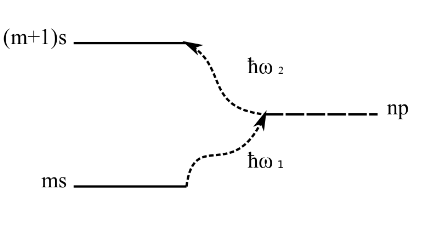
\includegraphics[width=0.4\textwidth]{images/transitioncrop.PNG}

\end{center}
        
In this particular example as our ground state is the \(1s\) state our intermediate virtual states are represented by the p states, as they are the only transitions allowed by parity. The classic method of solving this involves a summation over the entire spectrum of p states and then an integration of the positive continuum. This however is time consuming to do in practice. We instead will be using the pseudo-state method along with the variational method to deal with this.
	The main bulk of using this method is generating the pseudo states, to do this we first define what sort of function we wish to use. For our purposes we found that it is best to work in spherical coordinates as this makes the resulting integrals rather elegant to solve analytically. Every state is expanded in the basis set of functions \(r^n e^{-\alpha r}Y_l^m(\theta,\phi)\)\cite{shark}
	\begin{equation}
    \Psi(r)=\sum_{n=1}^{m}c_{n}r^{n}e^{-\alpha r}Y_{l}^{m}(\theta,\phi)
    =\sum_n c_n \chi_n
    \end{equation}
    \begin{equation}
        \chi_n=r^n e^{-\alpha r}Y_l^m(\theta,\phi)
    \end{equation}
    Where \(c_{n}\) is a linear variational parameter and \(\alpha\) is our nonlinear variational parameter. We use this particular form for our wave equations because the integrals can be solved analytically and rather simply.
    \begin{equation}
        \int_{0}^{\infty}r^{n}e^{-\alpha r}dr=\frac{n!}{\alpha^{n+1}}
    \end{equation}
 Firstly we must create out basis set by forming linear combinations. We do this by generating an overlap matrix whose elements are\cite{shark}.
 \begin{equation}
     \chi_{n}(r)=r^{n}e^{-\alpha r}Y_{l}^{m}(\theta,\phi)
 \end{equation}
 \begin{equation}
     O_{mn}=\bra{\chi_{m}}\ket{\chi_{n}}
 \end{equation}
  The way this matrix is orthogonalized is by the Jacobi method, which works in this case because our matrix is symmetric. For our matrix \(O\) we find the largest off diagonal element \(O_{nm}\). We then transform our matrix using a rotational matrix \(Q\) where\cite{jacobi}.
   \begin{equation}
     Q=\begin{bmatrix}
     1  &       &          &          &          &          &  \\
        &\hdots &          &          &          &          &  \\
        &       & \cos{(\theta)}  &\hdots   &-\sin{(\theta)}     & & \\  
        &       &\vdots &1      &\vdots & & \\  
                &       &\sin{(\theta)}   &\hdots   & \cos{(\theta)} & &\\
          &&&&&\hdots  \\    
            & & & & & &1
    \end{bmatrix}
 \end{equation}
  \begin{equation}
      \tan(2\theta)=\frac{O_{nm}}{O_{nn}-O_{mm}}
  \end{equation}
  This transformation is performed iteratively until all of the off diagonal elements are sufficiently small. We then set the total transformation matrix to \(T\) such that.
  \begin{equation}
      T=\prod_{i} Q_{i}
  \end{equation}

and
\begin{equation}
     T^{T}OT=\begin{bmatrix}
     I_{1}       & 0      & 0      &\hdots   & 0     \\
     0           & I_{2}  & 0      &\hdots   & 0     \\
     0           & 0      & I_{3}  &\hdots   & 0     \\  
    \vdots       & \vdots &\vdots  &\ddots   &\vdots \\  
     0           & 0      & 0      &\hdots   & I_{n} 
    \end{bmatrix}
 \end{equation}
Once the matrix is diagonalized we then apply a scalar change matrix to transform it to the identity matrix as follows
\begin{equation}
    S=\begin{bmatrix}
     \frac{1}{I_{1}^{\frac{1}{2}}}       & 0      & 0      &\hdots   & 0     \\
     0            &  \frac{1}{I_{2}^{\frac{1}{2}}}  & 0      &\hdots   & 0     \\
     0            & 0      &  \frac{1}{I_{3}^{\frac{1}{2}}}  &\hdots   & 0     \\  
     \vdots       & \vdots & \vdots  & \ddots  & \vdots \\  
     0            & 0      & 0       &\hdots   & \frac{1}{I_{n}^{\frac{1}{2}}} 
    
    
    \end{bmatrix}
\end{equation}
Where
\begin{equation}
    S^{t}T^{T}OTS=1
\end{equation}
We combine the two transformations as \(R=TS\) so that.
\begin{equation}
    R^{T}OR=1
\end{equation}
Once total transformation matrix is generated we then generate the Hamiltonian matrix of the form \(H_{nm}=\bra{\psi_{m}}H\ket{\psi_{n}}\) which we then express in our new basis set using our transformation matrix as follows
\begin{equation}
    H^{\prime}=R^{T}HR
\end{equation}
We then diagonalize our resulting matrix to give us our eigenvalues and eigenvectors for our basis set by applying an orthogonal transformation W.
\begin{equation}
    W^{T}H^{\prime}W=\begin{bmatrix}
    \lambda_{1} &0             &\hdots    &0 \\
    0           &\lambda_{2}   &\hdots    &0 \\
    \vdots      &\vdots        &\ddots    &\vdots \\
    0           &0             &0         &\lambda_{n}
    
    
                     \end{bmatrix}
\end{equation}
Our eigenvectors are given by applying our transformation matrices to the original wave equations, with the combination of R and W giving rise to the overall scale factor.
\begin{equation}
    \Psi^{q}(r)=
    \sum_{n,n^{\prime}}r^{n}e^{-\alpha r}Y_{l}^{m}(\theta,\phi)R_{n^{\prime},n}W_{n,q}
\end{equation}

Now that we have our new basis set we will be applying it to the calculation of the polarizability of hydrogen. We use the scenario of a hydrogen atom in the ground state within a static electric field of strength \textit{F} pointing in the \textit{z} direction. This gives rise to the perturbation of \(V=eFr\cos{\theta}\). Since we are working with hydrogen, the first order perturbation to the wave equations can be solved analytically. However this is a test of our pseudo-state method so we will be using that instead to calculate our second order correction to the energy. This is useful because we can use this very simple example to prove that our method works and can be applied to much more complex examples. Our pseudo-states \textit{n} will be applied in the following way to calculate the second order correction to the energy.
\begin{equation}
    E^{(2)}=\sum_{n=1}^{N}\frac{\abs{\bra{n_{p}}eFr\cos{\theta}\ket{1_{s}}}^{2}}{E_{1{s}}-E_{n}}
\end{equation}
Taking this with the definition of the dipole polarizability
\begin{equation}
    \alpha_{d}\equiv- E^{(2)}=\frac{9}{2}a_{0}^{3}
\end{equation}
We arrive at the correct answer of \(4.5a_{0}^{3}\).

There are several things worth mentioning about this technique. Firstly our variational parameter \(\alpha\). If we were to take our function for the dipole polarizability with a small basis set and plot is as a function of \(\alpha\) we can see that there is a rather significant variance. However we can very plainly see an absolute maximum located at \(\alpha=1\)\cite{variational}.  We can also see that there is an upper bound to our function and no matter how large we expand our basis set that ceiling of the true value of \(4.5a_{0}^{3}\) remains.

The one important thing that does change is our range of \(\alpha\) that will give us that result, as the functions ceiling tends to smooth out for larger basis sets as it is pressed against the true value. What this means is that, the larger our basis set, the more inaccurate our value for \(\alpha\) can be. When this method is applied to more complicated systems such as helium we can simply expand our basis set to larger and larger values to accommodate for our \(\alpha\). The main drawback is that the larger basis set used, the longer the computation time. Instead a much more economical technique is looking at the fact that our correct answer is located at the absolute maximum for our function. We can vary our \(\alpha\) to find this maximum to arrive at our ideal result. When working with more complicated systems it is far more economical to use these variational parameters find a maximum then it is to create a larger basis set.

For our purposes however we can arrive at our result of \(4.5a_{0}^{3}\) using only a two dimensional basis set\cite{variational}. This is extremely powerful as we are representing the entire spectrum of hydrogen with only two wave equations, greatly reducing our computing time.




\chapter{Sturmian Basis Sets}
Before we begin going into two-photon processes we must first develop a few computational techniques. When dealing with a two-photon process, the transition from initial to final state is connected by an intermediate state. This intermediate state is actually a summation over all possible bound states as well as an integration over the continuum. This is computationally very intensive and difficult to deal with. Instead we will be developing a technique that uses a discrete set of variational pseudostates to represent the entire spectrum of hydrogen. As a demonstration of this technique we will be showing how the entire spectrum of hydrogen can be represented by two pseudostates for the calculation of the polarizability. The particular calculation we will be doing to represent this is a calculation of the static polarizability of hydrogen. This is a known value that can be calculated analytically and so is a strong demonstration of the power of the technique.
\section{Sturmian Basis Sets}
The dipole polarizability of an atom corresponds to the zero-frequency limit of a two-photon process. \(\Delta E\) describes the energy shift of an atom in a static electric field according to
\begin{equation}
    \Delta E = \frac{1}{2}\alpha_d F^2
\end{equation}
Where \(F\) is the field strength and $\alpha_d$ is the polarizability. In this chapter we develop computational methods for this as a test case that will be applied later to two-photon processes. The dipole polarizability is defined by the second-order perturbation expression \cite{variational}
\begin{equation}
    \alpha_{d}\equiv- E^{(2)}=-\int\sum_{n=1}^{\infty}\frac{\abs{\bra{np}eFr\cos{\theta}\ket{1s}}^{2}}{E_{n}-E_{1s}}
\end{equation}
where the summation over $n$ includes an integration over the continuous part of the spectrum, and $E^{(2)}$ is the second-order perturbation energy due to the external field.
%The hyperfine transition that is being studied is a two photon process where the jump from the ground state to the excited state is mediated by a transition to an intermediate virtual state. This is represented as a summation over all possible states and an integration over the continuum. These two photons can be any frequency so long as the sum of their energies is equal to the total transition energy\cite{loudon}. There is no conservation of energy needed with regards to the intermediate states as no real transitions are occurring\cite{loudon}

%\begin{center}

%        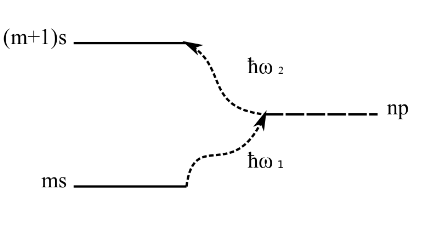
\includegraphics[width=0.4\textwidth]{images/transitioncrop.PNG}

%\end{center}
        
In this particular example the ground state is the \(1s\) state and the intermediate virtual states are represented by the p-states connected by electric dipole transitions. The expression as it stands involves a summation over the entire spectrum of p-states and then an integration over the continuum. This however is difficult to do in practice. We instead use the pseudostate method along with the variational method to sum over a discrete variational basis set with no integration over the continuum.
	The first set of using this method is generating the pseudostates. To do this we first define what sort of basis set we wish to use. Since the field-free Hamiltonian is spherically symmetric, we use spherical coordinates as this makes the resulting integrals rather elegant to evaluate analytically. Every state is expanded in the basis set of functions \(r^n e^{-\alpha r}Y_l^m(\theta,\phi)\) \cite{shark}
	\begin{equation}
    \Psi(r)=\sum_{n=1}^{N}c_{n}r^{n}e^{-\alpha r}Y_{l}^{m}(\theta,\phi)
    =\sum_n c_n \chi_n
    \end{equation}
    \begin{equation}
        \chi_n=r^n e^{-\alpha r}Y_l^m(\theta,\phi)
    \end{equation}
    where the \(c_{n}\) are linear variational parameters and \(\alpha\) is a nonlinear variational parameter. We use this particular form for our wave equations because they have the same functional form as hydrogenic wave functions. In addition, all integrals can be evaluated analytically using
    \begin{equation}
        \int_{0}^{\infty}r^{n}e^{-\alpha r}dr=\frac{n!}{\alpha^{n+1}}.
    \end{equation}
 First we must create out basis set by forming linear combinations. We do this by generating an overlap matrix whose elements are \cite{shark}.
 \begin{equation}
     \chi_{n}(r)=r^{n}e^{-\alpha r}Y_{l}^{m}(\theta,\phi)
 \end{equation}
 \begin{equation}
     O_{mn}=\bra{\chi_{m}}\ket{\chi_{n}}
 \end{equation}
  The way this matrix is orthogonalized is by the Jacobi method,(see Appendix) which works in this case because our matrix is symmetric. 

\section{Dipole Polarizability}
We now apply the sets of pseudostates to the calculation of the polarizability of ground-state hydrogen. We consider a hydrogen atom in the ground state placed in a static electric field of strength \textit{F} pointing in the \textit{z} direction. This gives rise to the perturbation \(V=eFr\cos{\theta}\). In the case of hydrogen, the first order perturbation equation can be solved analytically as further discussed below. However as a test of the pseudostate method, we will use it instead to calculate the second-order correction to the energy. This is useful because we can use this very simple example to test that the method works and can then be applied to much more complex examples. The $N$ pseudostates will be employed in the following way to calculate the second order correction to the energy.
\begin{equation}
    E^{(2)}=\sum_{n=1}^{N}\frac{\abs{\bra{n_{p}}eFr\cos{\theta}\ket{1s}}^{2}}{E_{n}-E_{1s}}
\end{equation}
Taking this with the definition of the dipole polarizability
\begin{equation}
    \alpha_{d}\equiv- E^{(2)}
\end{equation}
which for the case of the ground state of hydrogen becomes $\alpha_d=\frac{9}{2}a_{0}^{3}$ where $a_0$ is the Bohr radius. There are several things worth mentioning about this technique. The first concerns the variational parameter \(\alpha\). If we were to take our expression evaluated with a small basis set and plot is as a function of \(\alpha\) we can see that there is a rather significant variation as shown in Fig.\ref{fig:Dipole Polarizability}. However we can very plainly see an absolute maximum located at \(\alpha=1\) \cite{variational}.  We can also see that the true value of $\alpha_d$ is an upper bound to our function and no matter how large we expand our basis set that ceiling of the true value of \(4.5a_{0}^{3}\) is never exceeded. Note that all the contributions to Eq. (3.8) are positive.
\begin{figure}
    \centering
    \caption{Variational calculation of the dipole polarizability of 1s hydrogen with a two-term basis set}
    \label{fig:Dipole Polarizability}
\begin{tikzpicture}
\begin{axis}[
width=13cm,
height=10cm,
xlabel = Variational Parameter $\alpha$,
xmax = 1.4,
xmin = 0.45,
ylabel = Dipole Polarizability,
ymax = 4.5,
ymin = 4
]
\addplot[
color = black,
mark = none] table {Polar.txt};
\end{axis}
\end{tikzpicture}
\end{figure}

\begin{figure}
    \centering
    \caption{Stability of the polarizability with size of basis set}
    \label{fig:Dipole Polarizability MAXPOW}
\begin{tikzpicture}
\begin{axis}[
width=12cm,
height=10cm,
xlabel = Variational Parameter $\alpha$,
xmax = 2,
xmin = 0,
ylabel = Dipole Polarizability,
ymax = 4.55,
ymin = 0,
legend entries={$N=2$,$N=3$,$N=4$, $N=5$},
legend style={
cells={anchor=east},
legend pos=outer north east,
}
]
\addplot[
color = black,
mark = none] table {MAXPOW2.txt};
\addplot[
color = green,
mark = none] table {MAXPOW3.txt};
\addplot[
color = red,
mark = none] table {MAXPOW4.txt};
\addplot[
color = orange,
mark = none] table {MAXPOW5.txt};
\end{axis}
\end{tikzpicture}
\end{figure}
The one important thing that does change as $N$ increases is that the expression for $\alpha_d$ becomes less sensitive to the actual value of $\alpha$ used, as long as it is not too far from the optimum value $\alpha=1$. What this means is that, the larger the basis set, the less sensitively the calculated value for $\alpha_d$ depends on $\alpha$ as seen in Fig.\ref{fig:Dipole Polarizability MAXPOW}. When this method is applied to more complicated systems such as helium we can simply expand the basis set size and look for an extremum with respect to \(\alpha\). The main drawback is that the larger the basis set used, the longer the computation time. Instead a much more economical technique to look for a maximum for $\alpha_d$ as a function of $\alpha$. We can vary \(\alpha\) to find this maximum to arrive at the optimum result. When working with more complicated systems it is far more economical to use these variational parameters to find a maximum then it is to calculate using a larger basis set.

For our purposes however we can arrive at the exact result of \(4.5a_{0}^{3}\) using only a two dimensional basis set with matrix elements and energies of \cite{variational}
\begin{equation}
\begin{split}
    \psi_1&=re^{-r}-\sqrt{\frac{8}{45}}r^2 e^{-r}\\
    E_1&=-\frac{1}{10}\quad \rm{a.u.}\\
    \psi_2&=\sqrt{8} re^{-r}-2\frac{\sqrt{2}}{3}r^2 e^{-r}\\
    E_2&=\frac{1}{2}\quad \rm{a.u.}\\
\end{split}
\end{equation}
These were calculated using the Sturmian Basis set method as described in the previous section. This is extremely powerful as we are representing the entire spectrum of hydrogen with only two pseudostates.

\chapter{Two Photon Processes}
In this chapter we will begin reviewing the theories that are involved in a two-photon process. Two-photon processes come about through second-order perturbation theory so a brief description of it will allow for a greater understanding of the topic as a whole. We will be looking at how photons interact with matter to develop the operator we will be using in this study. From there we will be reviewing how time-orderings of the two photons is involved as well as how the basic theory works overall. This chapter will also discuss our results and derivation of the two-photon decay rate, how it relates to its two-photon Einstein B absorption coefficient and the results of it being applied to astrophysics. In addition to this we will be going over how it can be applied to Raman scattering as well as a brief discussion of how Raman and Rayleigh scattering differ from each other and other two-photon processes. Finally we will be presenting our results of all of these calculated values as they are scaled up through heavier hydrogenlike ions. 
\section{Second-Order Perturbation Theory}
Before discussing two-photon processes we must first discuss its root, being second-order perturbation theory. To begin we split up our Hamiltonian into two parts being \cite{variational}
\begin{equation}
\mathscr{H}=\mathscr{H}_0+\lambda\mathscr{H}_1
\end{equation}
where $\mathscr{H}_0$ is our unperturbed Hamiltonian which can be solved for analytically, and $V$ is our perturbation which is controlled by the parameter $\lambda$. We then expand our wave equations and energies in terms of our scale factor $\lambda$
\begin{equation}
    \begin{split}
        \Psi&=\Psi_0+\lambda\Psi_1+\lambda^2 \Psi_2\\
        E&=E_0+\lambda E_1+ \lambda^2 E_2
    \end{split}
\end{equation}
First-order perturbation was derived in a previous section so we will only focus on second-order perturbation here. Solving for the second order correction to the energy we have
\begin{equation}
    E_2=\frac{1}{\braket{\Psi_0}{\Psi_0}} \left[ 2\bra{\Psi_0}V\ket{\Psi_1}+2\bra{\Psi_0}H_0-E_0\ket{\Psi_2}+\bra{\Psi_1}H_0-E_0\ket{\Psi_1}\right]
\end{equation}
This is formed from terms with $\lambda^2$. $E_2$ is stable with respect to variations of $\Psi_2$, the second-order perturbation equation is
\begin{equation}
    (\mathscr{H}_0-E_0)\ket{\Psi_2}+ (V-E_1)\ket{\Psi_1}=E_2\ket{\Psi_0}
\end{equation}
then it follows that
\begin{equation}
    E_2=\frac{\bra{\Psi_0}V-E_1\ket{\Psi_1}}{\braket{\Psi_0}{\Psi_0}}
\end{equation}
and using the definition of $\Psi_1$ if it satisfies the first-order perturbation equation
\begin{equation}
    \ket{\Psi_1}= \frac{-(V-E_1)\ket{\Psi_0}}{H_0-E_0}
\end{equation}
we then multiply by unity 
\begin{equation}
    1=\int\sum_{n=1}^\infty \ket{\Psi n}\bra{\Psi n}
\end{equation}
to get our first-order perturbation to the wave equation as
\begin{equation}
    \ket{\Psi_1}=\int\sum_{n=1}^\infty \frac{\ket{\Psi n}\bra{\Psi n} -(V-E_1)\ket{\Psi_0}}{E_0 n-E_0}
\end{equation}
which we then substitute into our second-order perturbation to the energy to give
\begin{equation}
    E_2=\int\sum_{n=1}^\infty \frac{\bra{\Psi_0}V-E_1\ket{\Psi n}\bra{\Psi n} -(V-E_1)\ket{\Psi_0}}{E_0 n-E_0}
\end{equation}
For the particular case of solving the dipole polarizability for the s-state we use the fact that $E_1=0$ for the operator used is $V=Fr\cos{\theta}$. As detailed in previous sections we use a discrete basis set to represent the intermediate states, rather than summing over the entire spectrum and integrating over the continuum. The purpose of this derivation will be made obvious in the following sections, as the equation for the second-order perturbation is extremely similar to the matrix elements of a two-photon transition.

\section{Single-Photon Transitions}
In this section we will detail the derivation of the form of the interaction operator that we will be using in our two-photon transition. We first start from the definition of the Hamiltonian
\begin{equation}
    \mathscr{H}=\frac{p^2}{2m}+V
\end{equation}
through which we make the transformation to the canonical momentum
\begin{equation}
    \Vec{p}\rightarrow \Vec{p}-\frac{e}{c}\Vec{A}
\end{equation}
the Hamiltonian then becomes
\begin{equation}
    \begin{split}
            \mathscr{H}&=\frac{(\Vec{p}-\frac{e}{c}\Vec{A})^2}{2m}+V\\
            &=\frac{p^2}{2m}-\frac{e}{2mc}\Vec{p}\cdot\Vec{A}+\frac{e}{2mc}\Vec{A}\cdot\Vec{p}+\frac{e^2}{2mc^2}\Vec{A}^2+V
    \end{split}
\end{equation}
where
\begin{equation}
    \Vec{A}=A_0 \hat{e}e^{i\Vec{k}\cdot\Vec{r}-i\omega t}
\end{equation}
is the vector potential for a plane wave. Using the definition of a plane wave
\begin{equation}
    \abs{\Vec{k}}=\omega/c
\end{equation}
being of order $\alpha=1/c$ in atomic units and
\begin{equation}
    \Vec{k}\cdot\hat{e}=0
\end{equation}
for a transverse wave, we expand the Hamiltonian as
\begin{equation}
    \mathscr{H}= \frac{p^2}{2m}-\frac{2eA_0}{2mc}\Vec{p}\cdot\hat{e}[1-i\Vec{k}\cdot\Vec{r}+\cdots]e^{-i\omega t}
\end{equation}
Keeping only the first order term and using the fact that $\nabla\cdot A=0$ for a transverse wave we have
\begin{equation}
    \mathscr{H}_1=-\frac{eA_0}{2mc}2\Vec{p}\cdot\hat{e}
\end{equation}
We then calculate the transition matrix elements
\begin{equation}
    \bra{\Psi_i}\mathscr{H}_1\ket{\Psi_f}=\bra{\Psi_i}\Vec{p}\cdot\hat{e}\ket{\Psi_f}
\end{equation}
and use the commutator relation to get the operator into length form where
\begin{equation}
   \frac{m}{\hbar} \bra{\Psi_i}[\mathscr{H},\Vec{r}\cdot\hat{e}]\ket{\Psi_f}=\frac{m}{\hbar}(E_i-E_f)\bra{\Psi_i}\Vec{r}\cdot\hat{e}\ket{\Psi_f}
\end{equation}
This is the form of the interaction operator used in the next section for the two-photon transitions that are being studied. From this we can also show how energy is conserved. Using definitions for the time dependent portion of the wave equations where
\begin{equation}
    \Psi_i=e^{-iE_i t/\hbar}
\end{equation}
and
\begin{equation}
    \Psi_f=e^{-iE_f t/\hbar}
\end{equation}
This leads to the time integral
\begin{equation}
    \int_0^\infty(e^{-iE_i t/\hbar})^* e^{-i\omega t}e^{-iE_f  t/\hbar}dt=2\pi\delta\left(\frac{E_i}{\hbar}-\omega-\frac{E_f}{\hbar}\right)
\end{equation}
which leads to the conservation of energy relation
\begin{equation}
    \omega=(E_i-E_f)\hbar
\end{equation}
\section{Two-Photon Transitions}
Two-photon transitions come about through second-order perturbation theory \cite{loudon}. % with the second order perturbation taking the form of either \cite{mizushima1970quantum}
%\begin{equation}
%    P_{i\rightarrow f}=\frac{2\pi}{\hbar^2}\abs{\bra{f}\mathscr{H}\ket{i}}^2\delta(\omega_{if%})
%\end{equation}
%or
%\begin{equation}
%    P_{i\rightarrow f}=\frac{2\pi}{\hbar^2}
%    \abs{\frac{\bra{f}\mathscr{H}\ket{n}\bra{n}\mathscr{H}\ket{i}}
%    {\bra{n}\mathscr{H}\ket{n}-\bra{i}\mathscr{H}\ket{i}}}^2\delta(\omega_{if}).
%\end{equation}
%With $i$ and $f$ representing the initial and final states respectively, and $\omega_{if}$ representing the transition energy between the initial and final states.
%The first case is negligible due to both photons being absorbed by the system at the exact same time being a second order correction which has a much lower magnitude.The second scenario is far more probable as it is a first order correction and is what will be used in the analysis going forward.
The hyperfine transition that is being studied is a two-photon process where the transition from the ground state to the excited state is mediated by a transition to an intermediate virtual state $\ket{n}$ .These two photons can have any frequency $\omega$ so long as the sum of their energies $\hbar \omega_1+\hbar \omega_2$ is equal to the total transition energy.
\begin{center}

        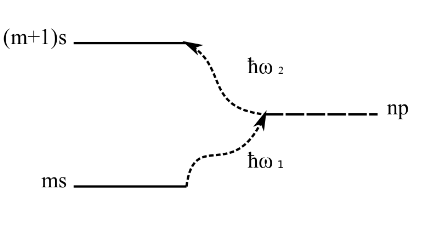
\includegraphics[width=0.4\textwidth]{images/transitioncrop.PNG}

\end{center}
The most probable atomic transitions involve emission or absorption of a single photon, where an atom starts in an initial state and then either absorbs or emits a single photon to go into either a higher or lower state respectively. We can represent this transition in bra-ket notation with the initial state $\ket{i}$ being operated on by the dipole operator \(\hat{e}\cdotp\Vec{r}\) to arrive at our final state $\ket{f}$. The dipole matrix element is then
\begin{equation}
    \bra{f}\hat{e}\cdotp\Vec{r}\ket{i}
\end{equation}
The construction of a two-photon transition is very similar. The major difference being that there is an intermediate virtual state in between the initial and final states. Starting with the initial state $\ket{i}$, operated on by \(\hat{\epsilon}\cdotp\Vec{r}\) to go to an intermediate virtual state $\bra{n}$. A second transition is then done by operating on the intermediate virtual state with \(\hat{\epsilon}\cdotp\Vec{r}\) to excite to the final state $\bra{f}$.
\begin{equation}
        \bra{f}\hat{e}\cdotp\Vec{r}\ket{n}\bra{n}\hat{e}\cdotp\Vec{r}\ket{i}
\end{equation}
The energies of the two photons do not have to be identical. The only constraint on them is that the sum of their energies must equal the transition energy from the initial state to the final state, due to conservation of energy. This brings up a unique problem in that the photons are not indistinguishable from each other. So the order in which the photons interact with the atom matter, and we must consider the three possible time-orderings that can occur.
\begin{figure}
    \centering
    \caption{Time orderings of a two-photon process}
    \label{fig:Timeorder}
    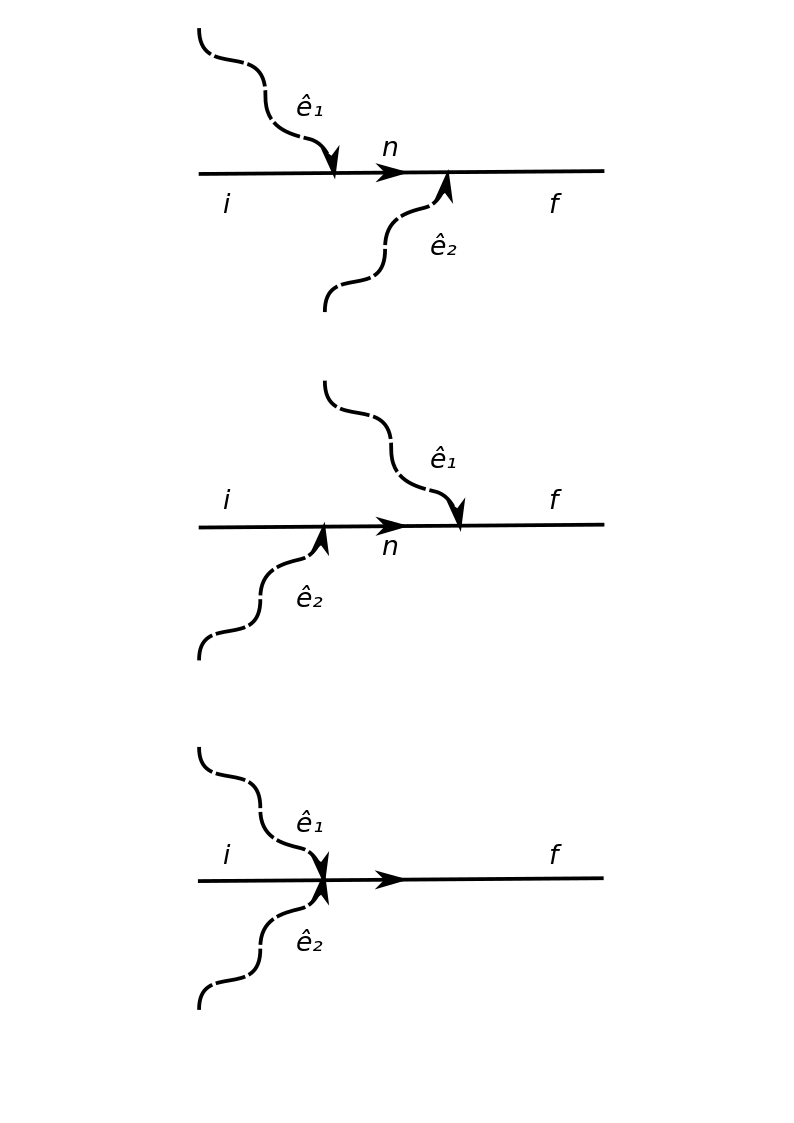
\includegraphics[width=0.4\textwidth]{images/twopproc.png}
\end{figure}

When talking about the different time-orderings in which two-photon processes can occur. it is assumed that the process happens instantly. The first time ordering shows the atom absorbing the first photon \(\hat{e}_1\), jumping to an intermediate state, absorbing the second photon \(\hat{e}_2\) and jumping to the final state. The second time ordering shows the same process except the order of the photons is reversed. The final time ordering shows both of the photons being absorbed simultaneously, this is a second order term and is therefore far less probable. The equation now changes to account for the specific order that the two photons are absorbed so that we average over the two time-orderings.
\begin{equation}
        \abs{
        \bra{f}\hat{e}_2\cdotp\Vec{r}\ket{n}
        \bra{n}\hat{e}_1\cdotp\Vec{r}\ket{i}
        +
        \bra{f}\hat{e}_1\cdotp\Vec{r}\ket{n}
        \bra{n}\hat{e}_2\cdotp\Vec{r}\ket{i}
        }^{2}
\end{equation}
We will specifically be considering a \(1s\) to \(2s\) transition in hydrogen using two photons. This transition is unique due to the the stability of the \(2s\) state giving rise to a lifetime of \(0.125\) s \cite{lifetime}, which is a tremendously long lifetime compared to other states. Due to parity, this transition can only occur through a two-photon decay so it is ideal as a demonstration. Using the previously built equations for two-photon processes along with the summation over pseudostates, from the previous chapter, our expression for the matrix elements of this transition is proportional to.
\begin{equation}
    \sum_{n} \abs{
    \frac{\bra{2s}z\ket{n}
    \bra{n}z\ket{1s}}
    {E_{n}-E_{0}+\omega_{1}}+
    \frac{\bra{2s}z\ket{n}
    \bra{n}z\ket{1s}}
    {E_{n}-E_{0}+\omega_{2}}
    }^{2}
\end{equation}
When considering the exchange of angular momentum going from a \(1s\) state where \(l=0\) to a \(2s\) where \(l=0\) the triangular rule tells us that the total angular momentum exchanged is 0. This is relevant due to the fact that each photon carries with it one unit of angular momentum. For this to occur the two photons are antiparallel thus the total angular momentum exchanged sum to zero. From this we calculate a full decay rate
\begin{equation}
    A(\nu_1)d\nu_1=\frac{1024\pi^6 e^4}{\hbar^2 c^4}\nu_1^3\nu_2^3
    \abs{(\hat{e}_1 \cdot \hat{e}_2)}^2
    \abs {\sum_{n} 
    \frac{\bra{2s}z\ket{n}
    \bra{n}z\ket{1s}}
    {E_{n}-E_{0}+\nu_{1}}+
    \frac{\bra{2s}z\ket{n}
    \bra{n}z\ket{1s}}
    {E_{n}-E_{0}+\nu_{2}}
    }^{2}
\end{equation}
with the total decay rate given by
\begin{equation}
    A=\frac{1}{2}\int_0^\nu A(\nu_1)d\nu_1
\end{equation}
where the factor of \(\frac{1}{2}\) is introduced because only unique pairs of photons are to be counted.
Observing the terms in this equations we see that the decay rate will be greatest when \(\omega_1 = \omega_2\) when the polarization of the polarization vectors are parallel or anti-parallel. This however will not be the case when considering this transition between the hyperfine levels being studied.

\section{Applications to Hyperfine Transitions in Hydrogen}
The hyperfine levels in ground-state hydrogen are represented by the eigenvectors
\begin{equation}
    \ket{1slsJIFM_f}
\end{equation}
with $s$ and $l$ representing the electrons spin and orbital angular momentum. These two angular momenta couple together to give the total angular momentum $J$ which is coupled with the spin of the nucleus $I$ to give the quantum number for hyperfine levels $F$. With \(M_f\) being the projection of $F$ onto the z-axis. The hyperfine levels of the ground state are separated into the two levels $F=0$ and $F=1$. Since this is a transition between two $s$ states, single-photon electric-dipole transitions are forbidden due to angular momentum and parity selection rules. Therefore two-photon processes are required. We will specifically be calculating the decay rate and absorption coefficient due to this process and will see if it is a potentially significant correction to astrophysical processes on cosmological distance scales. In addition to this, we will also be calculating cross sections for Raman scattering. For either of these processes we must first calculate the matrix elements using the equation
\begin{equation}
    \mathcal{M}^{-\gamma\gamma}(\hat{e}_i\rightarrow \hat{e}_f)=
    \sum_{n}
    \frac{
    \bra{f}\hat{e}_{2}\cdot
    \Vec{r}\ket{n}
    \bra{n}\hat{e}_{1}\cdot\Vec{r}\ket{i}}
    {\omega_{ni}+\omega_{1}}
    +
    \frac{
    \bra{f}\hat{e}_{1}\cdot\Vec{r}\ket{n}
    \bra{n}\hat{e}_{2}\cdot\Vec{r}\ket{i}}
    {\omega_{ni}+\omega_{2}}
\end{equation}
with both time-orderings of the photons being considered and all polarizations $\hat{e}$ of the two photons being accounted for by the dipole operator \(\hat{e}\cdot\Vec{r}\) where
\begin{equation}
    \hat{e_r}\cdot\Vec{r}= e_0r_0-e_+r_--e_-r_+
\end{equation}
\begin{equation}
    \begin{split}
        r_0&=z\\
        r_{\pm}&=\mp \frac{1}{\sqrt{2}}(x\pm iy)
    \end{split}
\end{equation}
\begin{equation}
    \begin{split}
        e_0&=e_z\\
        e_{\pm}&=\mp \frac{1}{\sqrt{2}}(e_x\pm ie_y)
    \end{split}
\end{equation}
and by conservation of energy
\begin{equation}
    \hbar \omega_1+\hbar \omega_2= E_i -E_f
\end{equation}
Summing this expression over all polarizations gives
\begin{equation}
\begin{split}
    \mathcal{M}^{-\gamma\gamma}(i\rightarrow f)=\\
    \sum_{\mu_1=-1}^1
    \sum_{\mu_2=-1}^1
    \sum_{n}
    (-1)^{\mu_2}(-1)^{\mu_1}
    \frac{
    \bra{f}{e}_{\mu_2}
    {r}_{-\mu_2}\ket{n}
    \bra{n}{e}_{\mu_1}{r}_{-\mu_1}\ket{i}}
    {\omega_{ni}+\omega_{1}}\\
    +(-1)^{\mu_1}(-1)^{\mu_2}
    \frac{
    \bra{f}{e}_{\mu_1}{r}_{-\mu_1}\ket{n}
    \bra{n}{e}_{\mu_2}{r_{-\mu_2}}\ket{i}}
    {\omega_{ni}+\omega_{2}}.
    \end{split}
\end{equation}
We may now include all the relevant quantum numbers for these transitions with the corresponding eigenvectors given by
\begin{equation}
    \ket{1s l s J I F M_f}
\end{equation}
for the initial state
\begin{equation}
    \ket{np l's'J'I'F'M_f'}
\end{equation}
as the intermediate state, and
\begin{equation}
        \bra{1s l'' s'' J'' I'' F'' M_f''}
\end{equation}
as the final state.
For the current purposes the only two quantum numbers that matter are the hyperfine splitting quantum number $F$ and its projection \(M_f\). The rest will be written together as \(\gamma\). We must also sum over all possible magnetic quantum numbers for the final states and  over the intermediate states with \(M_f''=-1,0,1\) and \(M_f'=-1,0,1\). Rewriting the transition equations gives us
\begin{equation}
\begin{split}
    \mathcal{M}^{-\gamma\gamma}(F\rightarrow F'')=
    \sum_{M_f''=-1}^1
    \sum_{M_f'=-1}^1
    \sum_{\mu_1=-1}^1
    \sum_{\mu_2=-1}^1
    \sum_{n}\\
    (-1)^{\mu_2}(-1)^{\mu_1}
    \frac{
    \bra{\gamma'' F'' M_F''}{e}_{\mu_2}
    {r}_{-\mu_2}\ket{\gamma' F' M_F'}
    \bra{\gamma' F' M_F'}{e}_{\mu_1}{r}_{-\mu_1}\ket{\gamma F M_F}}
    {\omega_{n0}+\omega_{1}}\\
    +(-1)^{\mu_1}(-1)^{\mu_2}
    \frac{
    \bra{\gamma'' F'' M_F''}{e}_{\mu_1}{r}_{-\mu_1}\ket{\gamma' F' M_F'}
    \bra{\gamma' F' M_F'}{e}_{\mu_2}{r_{-\mu_2}}\ket{\gamma F M_F}}
    {\omega_{n0}+\omega_{2}}.
    \end{split}
\end{equation}
To evaluate these matrix elements we first strip away the dependence on the magnetic quantum numbers by using the Wigner-Eckart theorem to calculate the reduced matrix element \cite{edmonds}
\begin{equation}
    (\gamma'j'm'\abs{T^k_q}\gamma jm)=(-1)^{j-m}
    \begin{pmatrix}
    j'  &k &j \\
    -m' &q &m
    \end{pmatrix}
    (\gamma'j'\abs{\abs{T^k}}\gamma j)
\end{equation}
or in this case
\begin{equation}
    (\gamma'F'M_f'\abs{r_{-\mu}}\gamma FM_F)=(-1)^{F-M_F}
    \begin{pmatrix}
    F'  &1 &F \\
    -M_F' &-\mu &M_F
    \end{pmatrix}
    (\gamma'F'\abs{\abs{r}}\gamma F)
\end{equation}
This changes our equation to
\begin{equation}
\begin{split}
    \mathcal{M}^{-\gamma\gamma}(F\rightarrow F'')=
    -\sqrt{\frac{1}{18}}\sum_{n}\\
    (e_2\cross e_1)
    \frac{
    (\gamma'' F''\abs{\abs{r}}\gamma' F')
    (\gamma' F'\abs{\abs{r}}\gamma F)}
    {\omega_{n0}+\omega_{1}}\\
    +(e_1\cross e_2)
    \frac{
    (\gamma'' F'' \abs{\abs{r}}\gamma' F')
    (\gamma' F'\abs{\abs{r}}\gamma F)}
    {\omega_{n0}+\omega_{2}}.
    \end{split}
\end{equation}
Using the fact that
\begin{equation}
    (e_1\cross e_2)=-(e_2\cross e_1)
\end{equation}
and that we must now strip away the dependence on the coupling of the total angular momentum with the spin of the nucleus we rewrite our equation as
\begin{equation}
\begin{split}
    \mathcal{M}^{-\gamma\gamma}(F\rightarrow F'')=
    -\sqrt{\frac{1}{18}} (e_2\cross e_1)\sum_{n}\sum_{J'=1/2}^{3/2}\\
    \frac{
    (\gamma''J''I'' F''\abs{\abs{r}}\gamma'J'I' F')
    (\gamma'J'I' F'\abs{\abs{r}}\gamma JI F)}
    {\omega_{n0}+\omega_{1}}\\
    -
    \frac{
    (\gamma''J''I'' F'' \abs{\abs{r}}\gamma'J'I' F')
    (\gamma'J'I' F'\abs{\abs{r}}\gamma JI F)}
    {\omega_{n0}+\omega_{2}}.
    \end{split}
\end{equation}
It is significant that as in the case of triplet helium decay \cite{dalgarnohelium} where one unit of angular momentum is exchanged in a two-photon process, the matrix element is proportional to the cross product of the polarization vectors, leading to a minus sign between the two terms. We now use the definition of a $6j$ symbol for two coupled angular momenta \cite{edmonds7}
\begin{equation}
\begin{split}
        (\gamma'j_1'j_2J'\abs{\abs{T(k)}}\gamma j_1 j_2 J)\\
        =(-1)^{j_1'+j_2+J+k}[(2J+1)(2J'+1)]^{\frac{1}{2}}
        \begin{Bmatrix}
        j_1' & J'  &j_2\\
        J    & j_1 &k
        \end{Bmatrix}
        (\gamma' j_1'\abs{\abs{T(k)}}\gamma j_1)
\end{split}
\end{equation}
In using this equation, we must take into consideration the fine structure splitting between the $J'=\frac{1}{2}$ and $J'=\frac{3}{2}$ p-states in hydrogen. Otherwise the two contributions cancel exactly. In addition to this we will apply the definition of the $6j$ symbol twice. First stripping away the dependence on the spin of the nucleus and second to strip away the dependence on the spin of the electron. This will give us a completely reduced matrix element
\begin{equation}
\begin{split}
    \mathcal{M}^{-\gamma\gamma}(i\rightarrow f)=
    \frac{1}{9}(e_2\cross e_1)
    \sum_{n}\\
    \frac{
    (1s\abs{\abs{r}}np)(np\abs{\abs{r}}1s)}     {\omega_{n_{\frac{3}{2}}0}+\omega_{1}}
    +
    \frac{
    (1s\abs{\abs{r}}np)(np\abs{\abs{r}}1s) }    {\omega_{n_{\frac{1}{2}}0}+\omega_{2}}\\
    -
    \frac{
    (1s\abs{\abs{r}}np)(np\abs{\abs{r}}1s) }    {\omega_{n_{\frac{1}{2}}0}+\omega_{1}}
    -
    \frac{
    (1s\abs{\abs{r}}np)(np\abs{\abs{r}}1s) }    {\omega_{n_{\frac{3}{2}}0}+\omega_{2}}
    \end{split}
\end{equation}
From here we can use the Wigner-Eckart theorem for $3j$ symbols to calculate the reduced matrix element
\begin{equation}
    (\gamma'j'\abs{\abs{T(k)}}\gamma j)=
    \frac{(\gamma'j'm'\abs{T(kq)}\gamma j m)}
    {
    (-1)^{j'-m'}
    \begin{pmatrix}
    j'  &k  &j\\
    -m' &q  &m
    \end{pmatrix}
    }
\end{equation}
For this we use the $z$ operator and \(m_l=0\) for the magnetic quantum numbers as it is convenient to calculate analytically. This changes the resulting equation to
\begin{equation}
\begin{split}
    \mathcal{M}^{-\gamma\gamma}(i\rightarrow f)=
    -\frac{1}{3}(e_2\cross e_1)
    \sum_{n}\bra{1s}z\ket{np}\bra{np}z\ket{1s}\\
    \bigg(
    \frac{1}{\omega_{p_{\frac{3}{2}}0}+\omega_{1}}
    +
    \frac{1} {\omega_{p_{\frac{1}{2}}0}+\omega_{2}}
    -
    \frac{1} {\omega_{p_{\frac{1}{2}}0}+\omega_{1}}
    -
    \frac{1} {\omega_{p_{\frac{3}{2}}0}+\omega_{2}}
    \bigg)
    \end{split}
\end{equation}
To display explicitly the difference between the $J'=\frac{1}{2}$ and $J'=\frac{3}{2}$ p-states, we find a common denominator. We also take the approximation that the fine structure splitting is relatively small compared to the other energy terms
\begin{equation}
     \frac{1}{\omega_{p_{\frac{3}{2}}0}+\omega}
     - \frac{1} {\omega_{p_{\frac{1}{2}}0}+\omega}
     =\frac{\omega_{3/2-1/2}}{\omega_{p0}^2+2\omega_{p0}\omega+\omega^2}
\end{equation}
where $\omega_{3/2-1/2}=\omega_{p_{\frac{3}{2}}0}-\omega_{p_{\frac{1}{2}}0}$ is the fine structure splitting. Some difficulty comes from calculating this value for a variational basis set. We use the equation for calculating the fine structure energy shift \cite{bethe}
\begin{equation}
    W_1=-\frac{\alpha^2Z^4}{2n^3}\left(\frac{1}{j+\frac{1}{2}}-\frac{3}{4n}\right)
\end{equation}
and evaluate the difference between two states where $j= \frac{3}{2}$ and $j=\frac{1}{2}$, we have the expression
\begin{equation}
    \omega_{p\frac{3}{2}-p\frac{1}{2}}=\frac{\alpha^2Z^4}{4n^3}
\end{equation}

Taking this into account and also considering the fact that the matrix elements are real numbers, the equation becomes 
\begin{equation}
\begin{split}
\mathcal{M}^{-\gamma\gamma}(i\rightarrow f)=
    -\frac{1}{3}(e_2\cross e_1)
    \sum_{n}\bra{np}z\ket{1s}^2\\
    \bigg(
    \frac{\omega_{3/2-1/2}}{\omega_{p0}^2+2\omega_{p0}\omega_1+\omega_1^2}
    -\frac{\omega_{3/2-1/2}}{\omega_{p0}^2+2\omega_{p0}\omega_2+\omega_2^2}
    \bigg)
    \end{split}
\end{equation}
which gives the final form for the matrix elements that will be used in the calculation of the decay rate, the absorption coefficient, and the Raman scattering cross section. We calculate this using a variational intermediate basis set with results being in Fig.\ref{fig:Calculation of the Transition Integrals}. As can be seen in the graph, the transition integral becomes zero when the frequencies of the two photons are equal.
\begin{figure}
    \centering
    \caption{Calculation of the transition integrals $\abs{\mathcal{M}^{-\gamma\gamma}(i\rightarrow f)}^2$}
    \label{fig:Calculation of the Transition Integrals}
\begin{tikzpicture}
\begin{axis}[ymin = 0, xlabel= $\omega/\Delta E$, ylabel=$\abs{\mathcal{M}^{-\gamma\gamma}(i\rightarrow f)}^2$, xmin=0, xmax=1, width=13cm,
height=10cm]
\addplot[
color = black,
mark = none] table {FancyM.txt};
\end{axis}
\end{tikzpicture}
\end{figure}
We will first apply this to the calculation of the decay rate using the equation \cite{dalgarnohelium}
\begin{equation}
    A(\nu_1)=\frac{1024\pi^6e^4}{h^2c^6}\nu_1^3\nu_2^3\abs{\mathcal{M}^{-\gamma\gamma}(i\rightarrow f)}^2
\end{equation}
which we change over to a form better suited for the program that we use, that form being as a relation of angular frequency $\omega$
\begin{equation}
     A(\omega_1)=\frac{16e^4}{c^6}\omega_1^3\omega_2^3\abs{\mathcal{M}^{-\gamma\gamma}(i\rightarrow f)}^2
\end{equation}
The evaluation of this function can be seen in Fig.\ref{fig:Calculation of the Decay Rate}.
\begin{figure}
    \centering
    \caption{Calculation of the decay rate A($\omega$)}
    \label{fig:Calculation of the Decay Rate}
\begin{tikzpicture}
\begin{axis}[ymin = 0, xlabel=$\omega/\Delta E$, ylabel= Decay Rate A($\omega$), xmin=0, xmax=1, width=13cm,
height=10cm]
\addplot[
color = black,
mark = none] table {Decay.txt};
\end{axis}
\end{tikzpicture}
\end{figure}
This equation must be integrated over all possible values for \(\omega\) to arrive at the full decay rate.
Due to the fact that
\begin{equation}
    \omega_2=\Delta E_{F=0 \rightarrow F=1}-\omega_1
\end{equation}
the double integration over $\omega_1$ and $\omega_2$ reduces to a single integral over $\omega_1$. In addition to this, due to the symmetric distribution about the mid point $\omega_1 = \omega_2$, we need only account for half of the total integral. This leaves us with the integral.
\begin{equation}
    A=\int_0^{\Delta E_{F=0 \rightarrow F=1}} A(\omega_1) d\omega_1
\end{equation}
which we integrate using the trapezoidal rule. This leads us to the result of
\begin{equation}
    A=1.97(3)\cross10^{-69}\rm{s}^{-1}
\end{equation}
which is an extremely small value. This value however is several orders of magnitude larger than the value calculated by V. P. Demidov. He approximated the value of this transition to be $7.6\cross10^{-73}\rm{s}^{-1}$ \cite{demidov1962two}. The stability of excited hyperfine ground state hydrogen leads to a lifetime of several million years in the single magnetic photon case \cite{lifetime}, but in this case it is several orders of magnitude greater than that. The stability of the calculation can be seen in Fig.\ref{fig:Calculation of the Decay Rate Variational} where it can be seen that the expression converges to an upper bound of the true value as the basis set is enlarged. For the polarizability we can represent the entire spectrum of hydrogen with a two-dimensional basis set. However in this case we need a much larger basis set due to the fine structure energy splitting being dependent on the basis set size.
\begin{figure}
    \centering
    \caption{Calculation of the decay rate A}
    \label{fig:Calculation of the Decay Rate Variational}
\begin{tikzpicture}
\begin{axis}[xlabel=Dimension of Basis set, ylabel= Decay Rate A, width=13cm,
height=10cm]
\addplot[
color = black,
mark = none] table {DecVar.txt};
\end{axis}
\end{tikzpicture}
\end{figure}

To acquire the absorption coefficient from this we must derive it using the Einstein A and B coefficients. This is done in a manner very similar to Woodgate's for the derivation of the Einstein A and B coefficients for a single-photon transition \cite{woodgate1}. We start from the loss rate $D$ and gain rate $N$ of the system \cite{Dehli}.
\begin{equation}
    \begin{split}
        D&=A+B_{22}\rho_1\rho_2+B_{21}\rho_2+B_{12}\rho_1\\
        N&=B_{11}\rho_1\rho_2\\
        \rho_i&= \left(\frac{8\pi h}{c^3}\right)(e^{h\nu_i/kT}-1)\nu_i^3
    \end{split}
\end{equation}
where $A$ is the spontaneous decay rate, $B_{22}$ is the doubly stimulated decay rate, $B_{12}$ and $B_{21}$ are the singly stimulated decay rates for the two separate photon orders and $B_{11}$ is the absorption coefficient. We then proceed to rearrange to get the absorption coefficient in terms of the decay rate
\begin{equation}
    \begin{split}
        \frac{N}{D}&=\left(\frac{A}{\rho_1 \rho_2} +B_{22}+\frac{B_{21}}{\rho_1}+\frac{B_{12}}{\rho_2}\right)^{-1}B_{11}\\
        &=e^{-\Delta E/kT}\left(\frac{g_2}{g_1}\right)\left(\frac{A}{\rho_1 \rho_2} +B_{22}+\frac{B_{21}}{\rho_1}+\frac{B_{12}}{\rho_2}\right)\\
        &=\left(\frac{c^3}{8\pi h}\right)^2 \frac{A}{\nu_1 ^3 \nu_2^3}+B_{22}+
        \left(\frac{c^3}{8\pi h}\right)\frac{B_{21}}{\nu_1^3}+\left(\frac{c^3}{8\pi h}\right)\frac{B_{12}}{\nu_2^3}\left(e^{h\nu_2 /kT}-1\right)\\
        &=\left(\frac{c^3}{8\pi h}\right)^2\left(e^{-\Delta E/kT} -e^{-h\nu_1 /kT}-e^{h\nu_2 /kT}+1 \right) \frac{A}{\nu_1 ^3 \nu_2^3}+B_{22}\\
        &+\left(\frac{c^3}{8\pi h}\right) \left( e^{h\nu_1 /kT}-1\right)\frac{B_{21}}{\nu_1^3}+\left(\frac{c^3}{8\pi h}\right) \left( e^{-h\nu_1 /kT}-1\right)\frac{B_{12}}{\nu_2^3}
    \end{split}
\end{equation}
we put
\begin{equation}
    \left(\frac{c^3}{8\pi h}\right)\frac{B_{21}}{\nu_1^3} = 
    \left(\frac{c^3}{8\pi h}\right)^2 \frac{A}{\nu_1^3 \nu_2^3}
\end{equation}
and
\begin{equation}
  \left(\frac{c^3}{8\pi h}\right)\frac{B_{12}}{\nu_2^3} = 
    \left(\frac{c^3}{8\pi h}\right)^2 \frac{A}{\nu_1^3 \nu_2^3}  
\end{equation}
then
\begin{equation}
\begin{split}
    B_{22}-\left(\frac{c^3}{8\pi h}\right) \frac{B_{21}}{\nu_1^3} - \left(\frac{c^3}{8\pi h}\right) \frac{B_{12}}{\nu_2^3}&=-\left(\frac{c^3}{8\pi h}\right)^2\frac{A}{\nu_1^3 \nu_2^3}\\
    B_{22}-\left(\frac{c^3}{8\pi h}\right)^2\frac{A}{\nu_1^3 \nu_2^3}-\left(\frac{c^3}{8\pi h}\right)^2\frac{A}{\nu_1^3 \nu_2^3}&=-\left(\frac{c^3}{8\pi h}\right)^2\frac{A}{\nu_1^3 \nu_2^3}
\end{split}
\end{equation}
which leads us to the result
\begin{equation}
    \left(\frac{g_2}{g_1}\right)B_{11}=\left(\frac{c^3}{8\pi h}\right)^2
    \frac{A}{\nu_1^3\nu_2^3}
\end{equation}
\begin{figure}
    \centering
    \caption{Calculation of the absorption coefficient B$_{11}$($\omega$)}
    \label{fig:Calculation of the Absorption Rate}
\begin{tikzpicture}
\begin{axis}[ymin = 0, xlabel=$\omega/\Delta E$, ylabel= Absorption coefficient, xmin=0, xmax=1, width=13cm,
height=10cm]
\addplot[
color = black,
mark = none] table {Absorb.txt};
\end{axis}
\end{tikzpicture}
\end{figure}
This equation along with the one for the decay rate gives an overall expression of
\begin{equation}
     B(\omega_1)=\frac{4\pi^2e^4}{\hbar^2}\abs{\mathcal{M}^{-\gamma\gamma}(i\rightarrow f)}^2
\end{equation}
This, similar to the decay rate gives us the function plotted in Fig.\ref{fig:Calculation of the Absorption Rate}. Using the same procedure of integrating over the bounds of the frequency leads us to an absorption coefficient of
\begin{equation}
    B_{11} = 5.28(4)\cross10^{-7} \rm{m^6 J^{-2} s^{-3}}
\end{equation}
Using this value we can calculate the gain rate of a system for several different scenarios using the expression for the gain rate
\begin{equation}
    N=B_{11}\rho_1\rho_2    
\end{equation}
where
\begin{equation}
    \rho_i=\left(\frac{8\pi h}{c^3}\right)(e^{h\nu_i/kT}-1)^{-1} \nu_i^3
\end{equation}
A logical starting point would be to look at how this transition effects the cosmic microwave background radiation where $T=2.72548\,\rm{K}$. Specifically we can look at individual frequencies for these cases. Due to the restriction that the two frequencies of the absorbed photons must sum up to the transition frequency, when we fix one we therefore fix the other by
\begin{equation}
    \omega_2=\omega_{HFS}-\omega_1
\end{equation}
This however does not remove this fact when we integrate over the frequency range where a delta function is present. When this occurs we simply use the fact that
\begin{equation}
    \int_{-\infty}^\infty f(x) \delta(y-x)dx=f(y)
\end{equation}
so we can simply evaluate our expression at the two frequencies we wish such that the total frequency is still equal to the hyperfine transition energy. This would lead to a total expression for the gain rate of
\begin{equation}
    N=\left(\frac{8\pi h}{c^3}\right)(e^{h\nu_i/kT}-1)^{-1} \nu_1^3
    \left(\frac{8\pi h}{c^3}\right)(e^{h\nu_i/kT}-1)^{-1} \nu_2^3
    \frac{4\pi^2e^4}{\hbar^2}\abs{\mathcal{M}^{-\gamma\gamma}(i\rightarrow f)}^2
\end{equation}
\begin{figure}
    \centering
    \caption{Calculation of the gain rate due to CMB radiation}
    \label{fig:gainrateCMB}
\begin{tikzpicture}
\begin{axis}[ymin = 0, xlabel=$\omega/\Delta E$, ylabel= Gain Rate $s^{-1}$, xmin=0, xmax=1, width=13cm,
height=10cm]
\addplot[
color = black,
mark = none] table {GAINCMB.txt};
\end{axis}
\end{tikzpicture}
\end{figure}
whose values can be seen in Fig.\ref{fig:gainrateCMB}. From this it can be seen that even over millions of years it will not be a significant correction to cosmic microwave background radiation.
\begin{figure}
    \centering
    \caption{Calculation of the gain rate due to CMB radiation and a star}
    \label{fig:gainrateCMBSUN}
\begin{tikzpicture}
\begin{axis}[ymin = 0, xlabel=$\omega/\Delta E$, ylabel= Gain Rate $s^{-1}$, xmin=0, xmax=1, width=13cm,
height=10cm]
\addplot[
color = black,
mark = none] table {GAINRATECMBSUN.txt};
\end{axis}
\end{tikzpicture}
\end{figure}
We can do another example where we consider the first photon coming from a sun-like surface of $T=5800\,\rm{K}$ and the second coming from the cosmic microwave background radiation. We can see the results of this in Fig.\ref{fig:gainrateCMBSUN} and can see that due to the function of the black-body radiation for the sun there is a distinct decrease in value for the second half of the frequencies.
\begin{figure}
    \centering
    \caption{Calculation of the gain rate due to a star}
    \label{fig:gainrateSUNSUN}
\begin{tikzpicture}
\begin{axis}[ymin = 0, xlabel=$\omega/\Delta E$, ylabel= Gain Rate $s^{-1}$, xmin=0, xmax=1, width=13cm,
height=10cm]
\addplot[
color = black,
mark = none] table {GAINRATESUNSUN.txt};
\end{axis}
\end{tikzpicture}
\end{figure}
The last scenario to look at would be assuming both photons come from a star and we can see in Fig.\ref{fig:gainrateSUNSUN} that we gain a significant order of magnitude as the temperature of the black body increases. However even over a cosmological time scale this sort of gain rate would still be very insignificant as a correction. This is logical due to the fact that even at higher temperatures the function for a black body is quite low for the relatively long wavelengths we are looking at.

\section{Raman Scattering}
A natural extension of this project would be to look at the hyperfine transition with respect to a Raman scattering process. Raman scattering was originally one of the first two-photon processes ever discovered and we will be seeing if the cross section is large enough for the hyperfine transition in the $1s$, state that it can be recreated in the lab. One thing worth noting for the transition integrals is the change to the denominator when considering scattering processes. Rayleigh and Raman scattering are two scattering processes that are very similar in nature. They each involve a system absorbing a photon, temporarily exciting to a virtual state and then decaying down to a different state. The main difference between Rayleigh and Raman scattering is that in Rayleigh scattering, when the system decays, it decays to the original state and the photon is of the same frequency as the one that was absorbed. This can be simply stated as Rayleigh scattering being an elastic process. In Raman scattering however the initial and final state are different and the photon that is emitted is of a different frequency to the one that was absorbed. This can be summed up as an inelastic process. In practice this will change the transitional integrals to account for the fact that the second photon is emitted instead of absorbed.
\begin{equation}
\begin{split}
\mathcal{M}^{-\gamma\gamma}(i\rightarrow f)=
    -\frac{1}{3}(e_2\cross e_1)
    \sum_{n}\bra{np}z\ket{1s}^2\\
    \bigg(
    \frac{\omega_{3/2-1/2}}{\omega_{p0}^2+2\omega_{p0}\omega_1+\omega_1^2}
    -\frac{\omega_{3/2-1/2}}{\omega_{p0}^2-2\omega_{p0}\omega_2+\omega_2^2}
    \bigg)
    \end{split}
\end{equation}
This change is to switch the usual plus sign next to the frequency of the photon with a minus sign. In addition to this the frequency of the absorbed photon is no longer bound by the transition energy. The photon can have any frequency so long as it is greater than the transition energy for the hyperfine splitting. The emitted photon however is bound by conservation of energy.
\begin{equation}
    \omega_2=\omega_1-\omega_{HFS}
\end{equation}
This is due to the fact that the process is inelastic and the energy is lost in the decay to a more excited state than the original. In addition to this a resonance term occurs as the frequency of the incident photon approaches the transition frequency to the first p-state so we will constrain our values for the absorbed photon below this \cite{4667}. The equation for the Raman scattering cross section is therefore \cite{dalgarnoraman}
\begin{equation}
    \sigma=\frac{(\alpha^2 m_e c^2)^28\pi a_0^2}{3(c)^4}\omega_1 \omega_2^3\abs{\mathcal{M}^{-\gamma\gamma}(i\rightarrow f)}^2
\end{equation}
\begin{figure}
    \centering
    \caption{Calculation of the Raman scattering cross section($\omega$)}
    \label{fig:Raman}
\begin{tikzpicture}
\begin{axis}[ymin = 0, xlabel=$\omega$ in a.u., ylabel= Raman Scattering Cross Section (yb), xmin=0, xmax=.375, width=13cm,
height=10cm]
\addplot[
color = black,
mark = none] table {RAMAN.txt};
\end{axis}
\end{tikzpicture}
\end{figure}
where $a_0$ is the Bohr radius and $m_e$ is the electron mass. We can see this plotted for energies below the resonance in Fig.\ref{fig:Raman}. As can be seen in the chart, a great deal of the cross section comes about as the frequency approaches resonance with the transition energy of the first excited pseudo p-state, that has a transition energy of $0.325$ a.u.
\begin{figure}
    \centering
    \caption{Calculation of the Raman scattering cross section($\omega$)}
    \label{fig:Ramanbelowres}
\begin{tikzpicture}
\begin{axis}[ymin = 0, xlabel=$\omega$ in a.u.,xtick={0.04, 0.08,0.12,0.16, 0.2}, ylabel= Raman Scattering Cross Section (yb), xmin=0, xmax=.2, width=14cm,
height=10cm]
\addplot[
color = black,
mark = none] table {RAMANBELOWRES.txt};
\end{axis}
\end{tikzpicture}
\end{figure}
A closer inspection of the values farther below resonance can be seen in Fig.\ref{fig:Ramanbelowres}. As can be seen there is a large exponential scaling with respect to the energy of the absorbed photon. 

Even with the increased energy range allowing frequencies that are beyond the hyperfine splitting transition our value for the theoretical Raman scattering cross section is very small. We can see that even across the entire frequency range below resonance we never leave the range of yoctobarns. It would be nearly impossible to see this phenomenon in the laboratory.

\section{Z-scaling}

As with most things calculated for hydrogen, these values can be extended to hydrogenlike ions. Due to the large scaling of the hyperfine transition frequency with $Z$ outstripping the general transition frequency, we are looking at heavier hydrogenlike ions to see if our values scale just as well.  To do this we look at the $Z$ scaling of the individual values. The transition operator in this case is
\begin{equation}
    z=r\cos{\theta}
\end{equation}
and we know that the particular Z scaling for r is
\begin{equation}
    r \propto \frac{1}{Z}
\end{equation}
and the energies have a Z scaling of
\begin{equation}
    E\propto \omega \propto Z^2
\end{equation}
Difficulty arises in extending this simple scale factor to the actual hyperfine splitting in hydrogenlike ions as although this value scales with $Z^3$ it is also dependent on the nuclear magnetic moment $\mu_N$ and the value for the spin of the nucleus $I$. These values do not have any set scaling so we will be using a combination of literature values as well as a fit to calculate the values for the hyperfine splitting in hydrogenic ions. For the purposes of this work we will be restricting ourselves to stable atoms as we wish to apply this to a laboratory setting. In addition to this due to complications with the coupling of $J$ and $I$ in the intermediate state we will be restricting ourselves further to only ions with nuclear spin $I=1/2$. However even with these restrictions we still have 23 separate ions to work with. Due to the location of the hyperfine splitting $\omega$ in the equation, we cannot simply apply an overall multiplying factor to our values and each must be computed individually for each ion. The scale factors that can be applied will be seen in the equation
\begin{equation}
\begin{split}
\mathcal{M}^{-\gamma\gamma}(i\rightarrow f)=
    -\frac{1}{3}(e_2\cross e_1)
    \sum_{n}\frac{1}{Z^2}\bra{np}z\ket{1s}^2\\
    \bigg(
    \frac{Z^4 \omega_{3/2-1/2}}{Z^4 \omega_{p0}^2+Z^2 2\omega_{p0}\omega_1+\omega_1^2}
    -\frac{Z^4 \omega_{3/2-1/2}}{Z^2 \omega_{p0}^2+Z^2 2\omega_{p0}\omega_2+\omega_2^2}
    \bigg)
    \end{split}
\end{equation}
When calculating the hyperfine splitting energy for the ground state we use the fact that the Fermi-contact term scales with $Z^3$ as well as with the nuclear magnetic moment $\mu_n$ so we can take a guess at the correct value through the equation
\begin{equation}
    \omega_{ZHFS}=\omega_{HHFS}*Z^3*\frac{\mu_n}{\mu_H}
\end{equation}
We then plotted and found the ratio between this experimental value with literature values, plotted this against $Z$ to find a rough overall multiplying factor to deal with the relativistic effects that become very prominent in heavy hydrogenic ions. Overall our final approximation of the hyperfine splitting frequency for hydrogenlike ions is
\begin{equation}
    \omega_{ZHFS}=\frac{\omega_{HHFS}Z^3\frac{\mu_n}{\mu_H}}{-0.00566Z+1.020373}
\end{equation}
 The results of this calculation for all stable isotopes with spin 1/2 can be seen in Table \ref{HFSZ}.

\begin{table}[h!]
  \begin{center}
    \caption{Hyperfine transition frequency for stable hydrogenlike isotopes with spin 1/2 nuclei.}
    \label{HFSZ}
    \pgfplotstabletypeset[
      multicolumn names, % allows to have multicolumn names
      col sep=comma, % the seperator in our .csv file
      display columns/0/.style={
		column name=Isotope, % name of first column
		column type={S},string type},  % use siunitx for formatting
      display columns/1/.style={
		column name=Hyperfine Transition Frequency (Hz),
        },
      every head row/.style={
		before row={\toprule}, % have a rule at top
		after row={
		% the units seperated by &
			\midrule} % rule under units
			},
		every last row/.style={after row=\bottomrule},
		] {HFSCALC3.csv} % filename/path to file
  \end{center}
\end{table}
With these approximated frequencies we apply it to the our calculation of the decay rate.
\begin{table}[h!]
  \begin{center}
    \caption{Ground state hyperfine two-photon decay rate for hydrogenlike stable isotopes with spin 1/2 nuclei.}
    \label{HFSDecayZ}
    \pgfplotstabletypeset[
      multicolumn names, % allows to have multicolumn names
      col sep=comma, % the seperator in our .csv file
      display columns/0/.style={
		column name=Isotope, % name of first column
		column type={S},string type},  % use siunitx for formatting
      display columns/1/.style={
		column name=Two Photon Decay Rate $s^{-1}$,
        },
      every head row/.style={
		before row={\toprule}, % have a rule at top
		after row={
		% the units seperated by &
			\midrule} % rule under units
			},
		every last row/.style={after row=\bottomrule},
		] {DecayZ.csv} % filename/path to file
  \end{center}
\end{table}
As can be seen from the results in Table \ref{HFSDecayZ} the value for the decay rate is several orders of magnitude higher as one moves up through the isotopes. However these values still result in lifetimes that are longer than the universe itself.

We can as before use the relationship between the Einstein $A$ and $B$ coefficient to arrive at $Z$-scaled values for the absorption coefficient B in Table \ref{HFSabsorbZ}. These values are reported in atomic units as they have dimensions that can be cumbersome and it seems to be the most clear way to report it. They have dimensions of $Distance^6 Energy^{-2} time^{-3}$.
\begin{table}[h!]
  \begin{center}
    \caption{Ground state hyperfine two-photon absorption coefficient for hydrogenlike stable isotopes with spin 1/2 nuclei.}
    \label{HFSabsorbZ}
    \pgfplotstabletypeset[
      multicolumn names, % allows to have multicolumn names
      col sep=comma, % the seperator in our .csv file
      display columns/0/.style={
		column name=Isotope, % name of first column
		column type={S},string type},  % use siunitx for formatting
      display columns/1/.style={
		column name=Two Photon Absorption Rate a.u.,
        },
      every head row/.style={
		before row={\toprule}, % have a rule at top
		after row={
		% the units seperated by &
			\midrule} % rule under units
			},
		every last row/.style={after row=\bottomrule},
		] {AbsorbZ.csv} % filename/path to file
  \end{center}
\end{table}
As can be seen in Table \ref{HFSabsorbZ} the values don't seem to change much as $Z$ is increased. This is likely due to the fact that the absorption coefficient does not scale as well with the hyperfine transition energy as it does with the overall energy difference between the ground state and the first intermediate state.

Finally we come to the Raman scattering cross sections that are scaled with $Z$. The values are dependent on the energy of the incident photon and the values that can be used for that frequency are all values below the first resonance frequency. That resonance point is the energy difference between the ground state and the first intermediate state. As can be seen from the various tables, although we do increase our cross section by several orders of magnitude as we move up through the periodic table, we do leave the range of yoctobarns. As such our cross section remains too low to be seen in the laboratory.
\begin{table}[h!]
  \begin{center}
    \caption{Raman scattering cross of the ground state hyperfine transition in hydrogenlike 2He3.}
    \label{R2He3}
    \pgfplotstabletypeset[
      multicolumn names, % allows to have multicolumn names
      col sep=comma, % the seperator in our .csv file
      display columns/0/.style={
		column name=Energy of the Absorbed Photon(a.u.), % name of first column
		column type={S},string type},  % use siunitx for formatting
      display columns/1/.style={
		column name=Cross Section (yb),
        },
      every head row/.style={
		before row={\toprule}, % have a rule at top
		after row={
		% the units seperated by &
			\midrule} % rule under units
			},
		every last row/.style={after row=\bottomrule},
		] {Raman/R2He3.csv} % filename/path to file
  \end{center}
\end{table}
\begin{table}[h!]
  \begin{center}
    \caption{Raman scattering cross of the ground state hyperfine transition in hydrogenlike 6C13.}
    \label{6He13}
    \pgfplotstabletypeset[
      multicolumn names, % allows to have multicolumn names
      col sep=comma, % the seperator in our .csv file
      display columns/0/.style={
		column name=Energy of the Absorbed Photon(a.u.), % name of first column
		column type={S},string type},  % use siunitx for formatting
      display columns/1/.style={
		column name=Cross Section (yb),
        },
      every head row/.style={
		before row={\toprule}, % have a rule at top
		after row={
		% the units seperated by &
			\midrule} % rule under units
			},
		every last row/.style={after row=\bottomrule},
		] {Raman/6C13.csv} % filename/path to file
  \end{center}
\end{table}
\begin{table}[h!]
  \begin{center}
    \caption{Raman scattering cross of the ground state hyperfine transition in hydrogenlike 7N15.}
    \label{7N15}
    \pgfplotstabletypeset[
      multicolumn names, % allows to have multicolumn names
      col sep=comma, % the seperator in our .csv file
      display columns/0/.style={
		column name=Energy of the Absorbed Photon(a.u.), % name of first column
		column type={S},string type},  % use siunitx for formatting
      display columns/1/.style={
		column name=Cross Section (yb),
        },
      every head row/.style={
		before row={\toprule}, % have a rule at top
		after row={
		% the units seperated by &
			\midrule} % rule under units
			},
		every last row/.style={after row=\bottomrule},
		] {Raman/7N15.csv} % filename/path to file
  \end{center}
\end{table}
\begin{table}[h!]
  \begin{center}
    \caption{Raman scattering cross of the ground state hyperfine transition in hydrogenlike 14Si29.}
    \label{14Si29}
    \pgfplotstabletypeset[
      multicolumn names, % allows to have multicolumn names
      col sep=comma, % the seperator in our .csv file
      display columns/0/.style={
		column name=Energy of the Absorbed Photon(a.u.), % name of first column
		column type={S},string type},  % use siunitx for formatting
      display columns/1/.style={
		column name=Cross Section (yb),
        },
      every head row/.style={
		before row={\toprule}, % have a rule at top
		after row={
		% the units seperated by &
			\midrule} % rule under units
			},
		every last row/.style={after row=\bottomrule},
		] {Raman/14Si29.csv} % filename/path to file
  \end{center}
\end{table}
\begin{table}[h!]
  \begin{center}
    \caption{Raman scattering cross of the ground state hyperfine transition in hydrogenlike 15P31.}
    \label{15P31}
    \pgfplotstabletypeset[
      multicolumn names, % allows to have multicolumn names
      col sep=comma, % the seperator in our .csv file
      display columns/0/.style={
		column name=Energy of the Absorbed Photon(a.u.), % name of first column
		column type={S},string type},  % use siunitx for formatting
      display columns/1/.style={
		column name=Cross Section (yb),
        },
      every head row/.style={
		before row={\toprule}, % have a rule at top
		after row={
		% the units seperated by &
			\midrule} % rule under units
			},
		every last row/.style={after row=\bottomrule},
		] {Raman/15P31.csv} % filename/path to file
  \end{center}
\end{table}
\begin{table}[h!]
  \begin{center}
    \caption{Raman scattering cross of the ground state hyperfine transition in hydrogenlike 26Fe57.}
    \label{26Fe57}
    \pgfplotstabletypeset[
      multicolumn names, % allows to have multicolumn names
      col sep=comma, % the seperator in our .csv file
      display columns/0/.style={
		column name=Energy of the Absorbed Photon(a.u.), % name of first column
		column type={S},string type},  % use siunitx for formatting
      display columns/1/.style={
		column name=Cross Section (yb),
        },
      every head row/.style={
		before row={\toprule}, % have a rule at top
		after row={
		% the units seperated by &
			\midrule} % rule under units
			},
		every last row/.style={after row=\bottomrule},
		] {Raman/26Fe57.csv} % filename/path to file
  \end{center}
\end{table}
\begin{table}[h!]
  \begin{center}
    \caption{Raman scattering cross of the ground state hyperfine transition in hydrogenlike 34Se77.}
    \label{34Se77}
    \pgfplotstabletypeset[
      multicolumn names, % allows to have multicolumn names
      col sep=comma, % the seperator in our .csv file
      display columns/0/.style={
		column name=Energy of the Absorbed Photon(a.u.), % name of first column
		column type={S},string type},  % use siunitx for formatting
      display columns/1/.style={
		column name=Cross Section (yb),
        },
      every head row/.style={
		before row={\toprule}, % have a rule at top
		after row={
		% the units seperated by &
			\midrule} % rule under units
			},
		every last row/.style={after row=\bottomrule},
		] {Raman/34Se77.csv} % filename/path to file
  \end{center}
\end{table}
\begin{table}[h!]
  \begin{center}
    \caption{Raman scattering cross of the ground state hyperfine transition in hydrogenlike 39Y89.}
    \label{39Y89}
    \pgfplotstabletypeset[
      multicolumn names, % allows to have multicolumn names
      col sep=comma, % the seperator in our .csv file
      display columns/0/.style={
		column name=Energy of the Absorbed Photon(a.u.), % name of first column
		column type={S},string type},  % use siunitx for formatting
      display columns/1/.style={
		column name=Cross Section (yb),
        },
      every head row/.style={
		before row={\toprule}, % have a rule at top
		after row={
		% the units seperated by &
			\midrule} % rule under units
			},
		every last row/.style={after row=\bottomrule},
		] {Raman/39Y89.csv} % filename/path to file
  \end{center}
\end{table}
\begin{table}[h!]
  \begin{center}
    \caption{Raman scattering cross of the ground state hyperfine transition in hydrogenlike 45Rh103.}
    \label{45Rh103}
    \pgfplotstabletypeset[
      multicolumn names, % allows to have multicolumn names
      col sep=comma, % the seperator in our .csv file
      display columns/0/.style={
		column name=Energy of the Absorbed Photon(a.u.), % name of first column
		column type={S},string type},  % use siunitx for formatting
      display columns/1/.style={
		column name=Cross Section (yb),
        },
      every head row/.style={
		before row={\toprule}, % have a rule at top
		after row={
		% the units seperated by &
			\midrule} % rule under units
			},
		every last row/.style={after row=\bottomrule},
		] {Raman/45Rh103.csv} % filename/path to file
  \end{center}
\end{table}
\begin{table}[h!]
  \begin{center}
    \caption{Raman scattering cross of the ground state hyperfine transition in hydrogenlike 47Ag109.}
    \label{47Ag109}
    \pgfplotstabletypeset[
      multicolumn names, % allows to have multicolumn names
      col sep=comma, % the seperator in our .csv file
      display columns/0/.style={
		column name=Energy of the Absorbed Photon(a.u.), % name of first column
		column type={S},string type},  % use siunitx for formatting
      display columns/1/.style={
		column name=Cross Section (yb),
        },
      every head row/.style={
		before row={\toprule}, % have a rule at top
		after row={
		% the units seperated by &
			\midrule} % rule under units
			},
		every last row/.style={after row=\bottomrule},
		] {Raman/47Ag109.csv} % filename/path to file
  \end{center}
\end{table}
\begin{table}[h!]
  \begin{center}
    \caption{Raman scattering cross of the ground state hyperfine transition in hydrogenlike 48Cd111.}
    \label{48Cd111}
    \pgfplotstabletypeset[
      multicolumn names, % allows to have multicolumn names
      col sep=comma, % the seperator in our .csv file
      display columns/0/.style={
		column name=Energy of the Absorbed Photon(a.u.), % name of first column
		column type={S},string type},  % use siunitx for formatting
      display columns/1/.style={
		column name=Cross Section (yb),
        },
      every head row/.style={
		before row={\toprule}, % have a rule at top
		after row={
		% the units seperated by &
			\midrule} % rule under units
			},
		every last row/.style={after row=\bottomrule},
		] {Raman/48Cd111.csv} % filename/path to file
  \end{center}
\end{table}
\begin{table}[h!]
  \begin{center}
    \caption{Raman scattering cross of the ground state hyperfine transition in hydrogenlike 50Sn115.}
    \label{50Sn115}
    \pgfplotstabletypeset[
      multicolumn names, % allows to have multicolumn names
      col sep=comma, % the seperator in our .csv file
      display columns/0/.style={
		column name=Energy of the Absorbed Photon(a.u.), % name of first column
		column type={S},string type},  % use siunitx for formatting
      display columns/1/.style={
		column name=Cross Section (yb),
        },
      every head row/.style={
		before row={\toprule}, % have a rule at top
		after row={
		% the units seperated by &
			\midrule} % rule under units
			},
		every last row/.style={after row=\bottomrule},
		] {Raman/50Sn115.csv} % filename/path to file
  \end{center}
\end{table}
\begin{table}[h!]
  \begin{center}
    \caption{Raman scattering cross of the ground state hyperfine transition in hydrogenlike 52Te125.}
    \label{52Te125}
    \pgfplotstabletypeset[
      multicolumn names, % allows to have multicolumn names
      col sep=comma, % the seperator in our .csv file
      display columns/0/.style={
		column name=Energy of the Absorbed Photon(a.u.), % name of first column
		column type={S},string type},  % use siunitx for formatting
      display columns/1/.style={
		column name=Cross Section (yb),
        },
      every head row/.style={
		before row={\toprule}, % have a rule at top
		after row={
		% the units seperated by &
			\midrule} % rule under units
			},
		every last row/.style={after row=\bottomrule},
		] {Raman/52Te125.csv} % filename/path to file
  \end{center}
\end{table}
\begin{table}[h!]
  \begin{center}
    \caption{Raman scattering cross of the ground state hyperfine transition in hydrogenlike 54Xe129.}
    \label{54Xe129}
    \pgfplotstabletypeset[
      multicolumn names, % allows to have multicolumn names
      col sep=comma, % the seperator in our .csv file
      display columns/0/.style={
		column name=Energy of the Absorbed Photon(a.u.), % name of first column
		column type={S},string type},  % use siunitx for formatting
      display columns/1/.style={
		column name=Cross Section (yb),
        },
      every head row/.style={
		before row={\toprule}, % have a rule at top
		after row={
		% the units seperated by &
			\midrule} % rule under units
			},
		every last row/.style={after row=\bottomrule},
		] {Raman/54Xe129.csv} % filename/path to file
  \end{center}
\end{table}
\begin{table}[h!]
  \begin{center}
    \caption{Raman scattering cross of the ground state hyperfine transition in hydrogenlike 69Tm169.}
    \label{69Tm169}
    \pgfplotstabletypeset[
      multicolumn names, % allows to have multicolumn names
      col sep=comma, % the seperator in our .csv file
      display columns/0/.style={
		column name=Energy of the Absorbed Photon(a.u.), % name of first column
		column type={S},string type},  % use siunitx for formatting
      display columns/1/.style={
		column name=Cross Section (yb),
        },
      every head row/.style={
		before row={\toprule}, % have a rule at top
		after row={
		% the units seperated by &
			\midrule} % rule under units
			},
		every last row/.style={after row=\bottomrule},
		] {Raman/69Tm169.csv} % filename/path to file
  \end{center}
\end{table}
\begin{table}[h!]
  \begin{center}
    \caption{Raman scattering cross of the ground state hyperfine transition in hydrogenlike 70Yb171.}
    \label{70Yb171}
    \pgfplotstabletypeset[
      multicolumn names, % allows to have multicolumn names
      col sep=comma, % the seperator in our .csv file
      display columns/0/.style={
		column name=Energy of the Absorbed Photon(a.u.), % name of first column
		column type={S},string type},  % use siunitx for formatting
      display columns/1/.style={
		column name=Cross Section (yb),
        },
      every head row/.style={
		before row={\toprule}, % have a rule at top
		after row={
		% the units seperated by &
			\midrule} % rule under units
			},
		every last row/.style={after row=\bottomrule},
		] {Raman/70Yb171.csv} % filename/path to file
  \end{center}
\end{table}
\begin{table}[h!]
  \begin{center}
    \caption{Raman scattering cross of the ground state hyperfine transition in hydrogenlike 74W183.}
    \label{74W183}
    \pgfplotstabletypeset[
      multicolumn names, % allows to have multicolumn names
      col sep=comma, % the seperator in our .csv file
      display columns/0/.style={
		column name=Energy of the Absorbed Photon(a.u.), % name of first column
		column type={S},string type},  % use siunitx for formatting
      display columns/1/.style={
		column name=Cross Section (yb),
        },
      every head row/.style={
		before row={\toprule}, % have a rule at top
		after row={
		% the units seperated by &
			\midrule} % rule under units
			},
		every last row/.style={after row=\bottomrule},
		] {Raman/74W183.csv} % filename/path to file
  \end{center}
\end{table}
\begin{table}[h!]
  \begin{center}
    \caption{Raman scattering cross of the ground state hyperfine transition in hydrogenlike 76Os187.}
    \label{76Os187}
    \pgfplotstabletypeset[
      multicolumn names, % allows to have multicolumn names
      col sep=comma, % the seperator in our .csv file
      display columns/0/.style={
		column name=Energy of the Absorbed Photon(a.u.), % name of first column
		column type={S},string type},  % use siunitx for formatting
      display columns/1/.style={
		column name=Cross Section (yb),
        },
      every head row/.style={
		before row={\toprule}, % have a rule at top
		after row={
		% the units seperated by &
			\midrule} % rule under units
			},
		every last row/.style={after row=\bottomrule},
		] {Raman/76Os187.csv} % filename/path to file
  \end{center}
\end{table}
\begin{table}[h!]
  \begin{center}
    \caption{Raman scattering cross of the ground state hyperfine transition in hydrogenlike 78Pt195.}
    \label{78Pt195}
    \pgfplotstabletypeset[
      multicolumn names, % allows to have multicolumn names
      col sep=comma, % the seperator in our .csv file
      display columns/0/.style={
		column name=Energy of the Absorbed Photon(a.u.), % name of first column
		column type={S},string type},  % use siunitx for formatting
      display columns/1/.style={
		column name=Cross Section (yb),
        },
      every head row/.style={
		before row={\toprule}, % have a rule at top
		after row={
		% the units seperated by &
			\midrule} % rule under units
			},
		every last row/.style={after row=\bottomrule},
		] {Raman/78Pt195.csv} % filename/path to file
  \end{center}
\end{table}
\begin{table}[h!]
  \begin{center}
    \caption{Raman scattering cross of the ground state hyperfine transition in hydrogenlike 80Hg199.}
    \label{80Hg199}
    \pgfplotstabletypeset[
      multicolumn names, % allows to have multicolumn names
      col sep=comma, % the seperator in our .csv file
      display columns/0/.style={
		column name=Energy of the Absorbed Photon(a.u.), % name of first column
		column type={S},string type},  % use siunitx for formatting
      display columns/1/.style={
		column name=Cross Section (yb),
        },
      every head row/.style={
		before row={\toprule}, % have a rule at top
		after row={
		% the units seperated by &
			\midrule} % rule under units
			},
		every last row/.style={after row=\bottomrule},
		] {Raman/80Hg199.csv} % filename/path to file
  \end{center}
\end{table}
\begin{table}[h!]
  \begin{center}
    \caption{Raman scattering cross of the ground state hyperfine transition in hydrogenlike 81Tl203.}
    \label{81Tl203}
    \pgfplotstabletypeset[
      multicolumn names, % allows to have multicolumn names
      col sep=comma, % the seperator in our .csv file
      display columns/0/.style={
		column name=Energy of the Absorbed Photon(a.u.), % name of first column
		column type={S},string type},  % use siunitx for formatting
      display columns/1/.style={
		column name=Cross Section (yb),
        },
      every head row/.style={
		before row={\toprule}, % have a rule at top
		after row={
		% the units seperated by &
			\midrule} % rule under units
			},
		every last row/.style={after row=\bottomrule},
		] {Raman/81Tl203.csv} % filename/path to file
  \end{center}
\end{table}
\begin{table}[h!]
  \begin{center}
    \caption{Raman scattering cross of the ground state hyperfine transition in hydrogenlike 82Pb207.}
    \label{82Pb207}
    \pgfplotstabletypeset[
      multicolumn names, % allows to have multicolumn names
      col sep=comma, % the seperator in our .csv file
      display columns/0/.style={
		column name=Energy of the Absorbed Photon(a.u.), % name of first column
		column type={S},string type},  % use siunitx for formatting
      display columns/1/.style={
		column name=Cross Section (yb),
        },
      every head row/.style={
		before row={\toprule}, % have a rule at top
		after row={
		% the units seperated by &
			\midrule} % rule under units
			},
		every last row/.style={after row=\bottomrule},
		] {Raman/82Pb207.csv} % filename/path to file
  \end{center}
\end{table}

%\renewcommand{\familydefault}{\sfdefault}

%\chapter{Wigner Eckhart Theorem}
%\input{Chapters/WignerEckhartTheorm}


%\chapter{Calculations}
%\input{Chapters/Calculation.tex}

\chapter{Conclusion}
This chapter will detail the future potential work for this project as well as some conclusions that can be gathered from the data. Starting off with our two-photon decay rate for the hyperfine transition in ground state hydrogen, we can see that our value leads to a lifetime of $10^{61}$ years. This is one of the longest lifetimes ever calculated in all of atomic physics. The significance is that it removes the need to include the decay rate as a source of uncertainty in cosmological applications, and hence it reduces the uncertainty. If we look back at how the single-photon decay of the excited hyperfine 1s state in hydrogen was used in astrophysics, we can see that even though the lifetime was several million years it was still significant over a galactic time scale. When considering the fact that the two photons can be of any frequency in the hyperfine range, if someone were to detect a photon from this process, they would have no idea if it were red shifted or blue shifted. 

We can see from the application of the absorption coefficient to the cosmic microwave background radiation that the gain rate is still extremely small. Even when considering cosmological distances this value would not lead to a great deal of lost photons. The Raman scattering coefficients are equally as small. When considering a cross section in yoctobarns, this would be extremely difficult to reproduce in the laboratory.

We also calculated these three values for all stable spin $1/2$ hydrogenlike isotopes up to bismuth. We scaled our calculations with the approximation of the hyperfine splitting in the ground state as well as the scaling to energy and distance relative to the Z value for the isotope. The decay rate was the most dramatically affected, increasing by almost 30 orders of magnitude relative to the hydrogen case. This is due to the fact that the decay rate has a rough scaling with the hyperfine splitting of $\omega^6$ so it was most affected. The absorption coefficient however has very little dependence on the hyperfine splitting and therefore only increased by a few orders of magnitude as it was scaled up with $Z$. The Raman scattering cross section scales with the energy of the absorbed and emitted photon. However these frequencies are dependent on the energy difference between the ground state and the first intermediate state. This caused the Raman scattering cross section to not scale as dramatically as the decay rate. although it increases by several orders of magnitude as it scales with $Z$, it never leaves the range of yoctobarns and is therefore likely not observable in the laboratory.

However there can likely be still more results that can be derived from this particular project. There are several isotopes that were not considered in this project. It would be beneficial to see if the angular momentum algebra for the isotopes without nuclear spin $1/2$ yield the same dependence on the fine structure energy splitting of the intermediate p-states. In our work we found that when summing over the values of $J$ for the intermediate p-states we arrived at a minus sign separating the two fine structure levels. If we did not consider the energy splitting between these two levels then the equation would become zero. It would be of interest to see if the same minus sign appears for a nuclear spin $3/2$ particle. If this is the case then all of the values calculated in this work would no longer depend on the fine structure energy of the intermediate p-states. For the case of hydrogen for the first excited state we have
\begin{equation}
    \omega_{p\frac{3}{2}-p\frac{1}{2}}=\frac{\alpha^2Z^4}{4n^3}=1.665\cross10^{-6}
\end{equation}
which squared leads to an overall multiplying factor of $10^{-12}$ to the first set of transitions integrals. If this is removed then we would increase the results by 12 orders of magnitude and would also open up a wide variety of hydrogenic isotopes to look at. \cite{demidov1962two}


\begin{appendices}
  \chapter{}
  \section{Hyperfine Angular Momentum Long Form}
The purpose of this appendix is to expand upon the derivation of the two-photon transition in the hyperfine levels of hydrogen. Beginning from the calculation of the transition integrals, we have
\begin{equation}
    \mathcal{M}^{-\gamma\gamma}(i\rightarrow f)=
    \sum_{n}
    \frac{
    \bra{f}\hat{e}_{2}\cdot
    \Vec{r}\ket{n}
    \bra{n}\hat{e}_{1}\cdot\Vec{r}\ket{i}}
    {\omega_{ni}-\omega_{1}}
    +
    \frac{
    \bra{f}\hat{e}_{1}\cdot\Vec{r}\ket{n}
    \bra{n}\hat{e}_{2}\cdot\Vec{r}\ket{i}}
    {\omega_{ni}-\omega_{2}}
\end{equation}
where
\begin{equation}
    \hat{e_r}\cdot\Vec{r}= e_0r_0-e_+r_--e_-r_+
\end{equation}
Considering all the quantum numbers that are necessary the initial state will be
\begin{equation}
    \bra{1s l s J I F M_f}
\end{equation}
with intermediate state
\begin{equation}
    \bra{np l's'J'I'F'M_f'}
\end{equation}
and final state
\begin{equation}
        \bra{1s l'' s'' J'' I'' F'' M_f''}
\end{equation}
Consider only on one of the state combinations
\begin{align}
\begin{split}
        \bra{1s l'' s'' J'' I'' F'' M_f''}
    e_{20}r_0-e_{2+}r_--e_{2-}r_+
    \ket{np l's'J'I'F'M_f'}\\
    \cross\bra{np l's'J'I'F'M_f'}
    e_{10}r_0-e_{1+}r_--e_{1-}r_+
    \ket{1s l s J I F M_f}
\end{split}
\end{align}
Breaking up these equations for ease of use into
\begin{align}
\begin{split}
    \bra{1s l'' s'' J'' I'' F'' M_f''}
    e_{20}r_0
    \ket{np l's'J'I'F'M_f'}\\
    -\bra{1s l'' s'' J'' I'' F'' M_f''}
    e_{2+}r_-
    \ket{np l's'J'I'F'M_f'}\\
    -\bra{1s l'' s'' J'' I'' F'' M_f''}
    e_{2-}r_+
    \ket{np l's'J'I'F'M_f'}
\end{split}
\end{align}
we then use the Wigner Eckart theorem in the form \cite{edmonds}
\begin{equation}
    (\gamma'j'm'\abs{T^k_q}\gamma jm)=(-1)^{j-m}
    \begin{pmatrix}
    j'  &k &j \\
    -m' &q &m
    \end{pmatrix}
    (\gamma'j'\abs{\abs{T^k}}\gamma j)
\end{equation}
to break up (A.7) into its reduced matrix element and 3j symbols
\begin{align}
\begin{split}
    \bra{1s l'' s'' J'' I'' F'' M_f''}
    e_{20}r_0
    \ket{np l's'J'I'F'M_f'}\\
    -\bra{1s l'' s'' J'' I'' F'' M_f''}
    e_{2+}r_-
    \ket{np l's'J'I'F'M_f'}\\
    -\bra{1s l'' s'' J'' I'' F'' M_f''}
    e_{2-}r_+
    \ket{np l's'J'I'F'M_f'}\\
    =(1sl'' s'' J'' I'' F''\abs{\abs{r}}np l's'J'I'F')(-1^{F'-M_f'})\\
    \cross[
    (e_{20})
    \begin{pmatrix}
    F''    & 1 & F'\\
    -M_f'' & 0 &M_f'
    \end{pmatrix}
    -
    (e_{2-})
    \begin{pmatrix}
    F''    & 1  & F'\\
    -M_f'' & -1 &M_f'
    \end{pmatrix}
    -
    (e_{2+})
    \begin{pmatrix}
    F''    & 1 & F'\\
    -M_f'' & 1 &M_f'
    \end{pmatrix}
    ]
\end{split}
\end{align}
We do the same thing for the first photon.
\begin{align}
\begin{split}
    \bra{np l' s' J' I' F' M_f'}
    e_{20}r_0
    \ket{1s lsJIFM_f}\\
    -\bra{np l' s' J' I' F' M_f'}
    e_{2+}r_-
    \ket{1s lsJIFM_f}\\
    -\bra{np l' s' J' I' F' M_f'}
    e_{2-}r_+
    \ket{1s lsJIFM_f}\\
    =(npl' s' J' I' F'\abs{\abs{r}}1s lsJIF)(-1^{F-M_f})\\
    \cross[
    (e_{10})
    \begin{pmatrix}
    F'    & 1 & F\\
    -M_f' & 0 &M_f
    \end{pmatrix}
    -
    (e_{1-})
    \begin{pmatrix}
    F'    & 1  & F\\
    -M_f' & -1 &M_f
    \end{pmatrix}
    -
    (e_{1+})
    \begin{pmatrix}
    F'    & 1 & F\\
    -M_f' & 1 &M_f
    \end{pmatrix}
    ]
\end{split}
\end{align}
As above these two equations are multiplied together.
\begin{align}
    \begin{split}
            =(1sl'' s'' J'' I'' F''\abs{\abs{r}}npl's'J'I'F')
            (npl' s' J' I' F'\abs{\abs{r}}1s lsJIF)
            (-1^{F'-M_f'})(-1^{F-M_f})\\
            \cross
            [
            (e_{20}e_{10})
            \begin{pmatrix}
             F''    & 1 & F'\\
            -M_f'' & 0 &M_f'
            \end{pmatrix}
            \begin{pmatrix}
            F'    & 1 & F\\
            -M_f' & 0 &M_f
            \end{pmatrix}\\
            -
            (e_{20}e_{1+})
            \begin{pmatrix}
             F''    & 1 & F'\\
            -M_f'' & 0 &M_f'
            \end{pmatrix}
            \begin{pmatrix}
            F'    & 1 & F\\
            -M_f' & -1 &M_f
            \end{pmatrix}\\
            -
            (e_{20}e_{1-})
            \begin{pmatrix}
             F''    & 1 & F'\\
            -M_f'' & 0 &M_f'
            \end{pmatrix}
            \begin{pmatrix}
            F'    & 1 & F\\
            -M_f' & 1 &M_f
            \end{pmatrix}\\
            -
            (e_{2+}e_{10})
            \begin{pmatrix}
             F''    & 1 & F'\\
            -M_f'' & -1 &M_f'
            \end{pmatrix}
            \begin{pmatrix}
            F'    & 1 & F\\
            -M_f' & 0 &M_f
            \end{pmatrix}\\
            +
            (e_{2+}e_{1+})
            \begin{pmatrix}
             F''    & 1 & F'\\
            -M_f'' & -1 &M_f'
            \end{pmatrix}
            \begin{pmatrix}
            F'    & 1 & F\\
            -M_f' & -1 &M_f
            \end{pmatrix}\\
            -
            (e_{2+}e_{1-})
            \begin{pmatrix}
             F''    & 1 & F'\\
            -M_f'' & -1 &M_f'
            \end{pmatrix}
            \begin{pmatrix}
            F'    & 1 & F\\
            -M_f' & 1 &M_f
            \end{pmatrix}\\
            -
            (e_{2-}e_{10})
            \begin{pmatrix}
             F''    & 1 & F'\\
            -M_f'' & 1 &M_f'
            \end{pmatrix}
            \begin{pmatrix}
            F'    & 1 & F\\
            -M_f' & 0 &M_f
            \end{pmatrix}\\
            +
            (e_{2-}e_{1+})
            \begin{pmatrix}
             F''    & 1 & F'\\
            -M_f'' & 1 &M_f'
            \end{pmatrix}
            \begin{pmatrix}
            F'    & 1 & F\\
            -M_f' & -1 &M_f
            \end{pmatrix}\\
            +
            (e_{2-}e_{1-})
            \begin{pmatrix}
             F''    & 1 & F'\\
            -M_f'' & 1 &M_f'
            \end{pmatrix}
            \begin{pmatrix}
            F'    & 1 & F\\
            -M_f' & 1 &M_f
            \end{pmatrix}
            ]
    \end{split}
\end{align}
We then set our values of our quantum numbers to those that are allowed by the triangular rule \(F''=F'=1\) and \(F=0\) and sum over the magnetic quantum numbers.
\begin{align}
    \begin{split}
            =\sum_{M_f'=-1}^1\sum_{M_f=-1}^1
            (1sl'' s'' J'' I'' 1\abs{\abs{r}}npl's'J'I'1)
            (npl' s' J' I' 1\abs{\abs{r}}1s lsJI0)\\
            \cross (-1^{F'-M_f'})(-1^{F-M_f})\\
            \cross
            [
            (e_{20}e_{10})
            \begin{pmatrix}
             1    & 1 & 1\\
            -M_f'' & 0 &M_f'
            \end{pmatrix}
            \begin{pmatrix}
            1    & 1 & 0\\
            -M_f' & 0 &M_f
            \end{pmatrix}\\
            -
            (e_{20}e_{1+})
            \begin{pmatrix}
             1    & 1 & 1\\
            -M_f'' & 0 &M_f'
            \end{pmatrix}
            \begin{pmatrix}
            1    & 1 & 0\\
            -M_f' & -1 &M_f
            \end{pmatrix}\\
            -
            (e_{20}e_{1-})
            \begin{pmatrix}
             1    & 1 & 1\\
            -M_f'' & 0 &M_f'
            \end{pmatrix}
            \begin{pmatrix}
            1    & 1 & 0\\
            -M_f' & 1 &M_f
            \end{pmatrix}\\
            -
            (e_{2+}e_{10})
            \begin{pmatrix}
             1    & 1 & 1\\
            -M_f'' & -1 &M_f'
            \end{pmatrix}
            \begin{pmatrix}
            1    & 1 & 0\\
            -M_f' & 0 &M_f
            \end{pmatrix}\\
            +
            (e_{2+}e_{1+})
            \begin{pmatrix}
             1    & 1 & 0\\
            -M_f'' & -1 &M_f'
            \end{pmatrix}
            \begin{pmatrix}
            1    & 1 & 0\\
            -M_f' & -1 &M_f
            \end{pmatrix}\\
            -
            (e_{2+}e_{1-})
            \begin{pmatrix}
             1    & 1 & 1\\
            -M_f'' & -1 &M_f'
            \end{pmatrix}
            \begin{pmatrix}
            1    & 1 & 0\\
            -M_f' & 1 &M_f
            \end{pmatrix}\\
            -
            (e_{2-}e_{10})
            \begin{pmatrix}
             1    & 1 & 1\\
            -M_f'' & 1 &M_f'
            \end{pmatrix}
            \begin{pmatrix}
            1    & 1 & 0\\
            -M_f' & 0 &M_f
            \end{pmatrix}\\
            +
            (e_{2-}e_{1+})
            \begin{pmatrix}
             1    & 1 & 1\\
            -M_f'' & 1 &M_f'
            \end{pmatrix}
            \begin{pmatrix}
            1    & 1 & 0\\
            -M_f' & -1 &M_f
            \end{pmatrix}\\
            +
            (e_{2-}e_{1-})
            \begin{pmatrix}
             1    & 1 & 1\\
            -M_f'' & 1 &M_f'
            \end{pmatrix}
            \begin{pmatrix}
            1    & 1 & 0\\
            -M_f' & 1 &M_f
            \end{pmatrix}
            ]
    \end{split}
\end{align}

Summing all the possible magnetic quantum numbers will give us 81 separate terms of which only 6 terms survive due to our selection rules
\begin{equation}
\abs{j-k}\leq j'\leq\abs{j+k}
\end{equation}
and 
\begin{equation}
    m+q=m'
\end{equation}
if
\begin{equation}
  m=m'=q=0  
\end{equation}
then
\begin{equation}
    j'+k+j=2k
\end{equation}
Where \(k\in \mathbb{Z}\)

After calculating all the coefficients of the surviving terms we are left with
\begin{equation}
    \begin{split}
        =\sqrt{\frac{1}{18}
        }(1sl'' s'' J'' I'' 1\abs{\abs{r}}npl's'J'I'1)
        (npl' s' J' I' 1\abs{\abs{r}}1s lsJI0)\\
        (e_{20}e_{1+}-e_{2+}e_{10}+e_{2-}e_{1+}-
        e_{2+}e_{1-}+e_{2-}e_{10}-e_{20}e_{1-})
    \end{split}    
\end{equation}
where
\begin{equation}
    (e_{20}e_{1+}-e_{2+}e_{10}+e_{2-}e_{1+}-
        e_{2+}e_{1-}+e_{2-}e_{10}-e_{20}e_{1-})=(e_2\cross e_1)
\end{equation}
Giving the same treatment to the case in which photon 2 is absorbed before photon 1 we arrive at a similar equation except the cross product is the opposite order. We then use the fact that
\begin{equation}
e_1\cross e_2=-e_2\cross e_1    
\end{equation}
This effect shows that this process cannot occur if the two photons being absorbed or emitted have the same energy. We know this intuitively through the angular momentum selection rules by the fact that the process with $\Delta F=1$ transports only one unit of angular momentum, whereas two photons of the exact energy emitted back-to-back can transport only zero or two units of angular momentum. Returning to our master equation we can see all the changes we have made.
\begin{equation}
\begin{split}
    \mathcal{M}^{-\gamma\gamma}(i\rightarrow f)=\\
    (e_2\cross e_1)(\sqrt{\frac{1}{18}})
    \sum_{n}
    \frac{
    (1s\gamma '' J'' I'' 1\abs{\abs{r}}np\gamma J'I'1)
    (np\gamma ' J' I' 1\abs{\abs{r}}1s \gamma JI0)}
    {\omega_{n0}-\omega_{1}}\\
       -
    \frac{
    (1s\gamma '' J'' I'' 1\abs{\abs{r}}np\gamma J'I'1)
    (np \gamma J' I' 1\abs{\abs{r}}1s \gamma JI0)}
    {\omega_{n0}-\omega_{2}}
    \end{split}
\end{equation}
However we still need to strip out the dependence on the coupled spin of the proton \(I\) with total angular momenta \(J\) to give hyperfine \(F\) as well as the dependence of electron spin\(s\). To do this we used the version of the Wigner Eckart Theorem.
\begin{equation}
\begin{split}
        (\gamma'j_1'j_2J'\abs{\abs{T(k)}}\gamma j_1 j_2 J)\\
        =(-1)^{j_1'+j_2+J+k}[(2J+1)(2J'+1)]^{\frac{1}{2}}
        \begin{Bmatrix}
        j_1' & J'  &j_2\\
        J    & j_1 &k
        \end{Bmatrix}
        (\gamma' j_1'\abs{\abs{T(k)}}\gamma j_1)
\end{split}
\end{equation}
and apply it to our bra-ket pairs to give
\begin{equation}
\begin{split}
        (\gamma''J''IF''\abs{\abs{r}}\gamma' J' I F')\\
        =(-1)^{J''+I+F''+1}[(2F'+1)(2F''+1)]^{\frac{1}{2}}
        \begin{Bmatrix}
        J'' & F''  &I\\
        F'    & J' &1
        \end{Bmatrix}
        (1sl''s'' J''\abs{\abs{r}}np l's' J')
\end{split}
\end{equation}
and
\begin{equation}
\begin{split}
        (\gamma'J'IF'\abs{\abs{r}}\gamma J I F)\\
        =(-1)^{J'+I+F'+1}[(2F+1)(2F'+1)]^{\frac{1}{2}}
        \begin{Bmatrix}
        J' & F'  &I\\
        F    & J &1
        \end{Bmatrix}
        (np l' s' J'\abs{\abs{r}}1s ls J)
\end{split}
\end{equation}
We then apply the same Wigner Eckart theorem a second time, except this time stripping out dependence on spin \(s\) and total angular momentum \(J\). Multiplying the two equations together results in.
\begin{equation}
    \begin{split}
        (1sl'' s'' J'' I'' 1\abs{\abs{r}}npl's'J'I'1)
        (npl' s' J' I' 1\abs{\abs{r}}1s lsJI0)=\\
        (-1)^{J'+I+F'+k+J''+I+F''+k}\\
        [(2F+1)(2F'+1)]^{\frac{1}{2}}
         [(2F'+1)(2F''+1)]^{\frac{1}{2}}
         [(2J+1)(2J'+1)]^{\frac{1}{2}}
         [(2J'+1)(2J''+1)]^{\frac{1}{2}}\\
        \begin{Bmatrix}
        J' & F'  &I\\
        F    & J &1
        \end{Bmatrix}
        \begin{Bmatrix}
        J'' & F''  &I\\
        F'    & J' &1
        \end{Bmatrix}
        \begin{Bmatrix}
        l' & J'  &s\\
        J    & l &k
        \end{Bmatrix}
        \begin{Bmatrix}
        l'' & J''  &s\\
        J'    & l' &k
        \end{Bmatrix}
        (1sl''\abs{\abs{r}}npl')(npl'\abs{\abs{r}}1sl)
    \end{split}
\end{equation}
We then substitute in the angular quantum numbers \(F=0\), \(F'=F''=1\), \(I=\frac{1}{2}\), \(s=\frac{1}{2}\), \(l=l''=0\), \(l'=1\), and sum over our possible total angular momenta for our intermediate p states with \(J=\frac{1}{2}\quad \rm{or} \quad \frac{3}{2}\). The last part in particular causes us to arrive at a very interesting result
\begin{equation}
    \begin{split}
        (1sl'' s'' J'' I'' F''\abs{\abs{r}}npl's'J'I'F')
        (npl' s' J' I' F'\abs{\abs{r}}1s lsJIF)=\\
        {\frac{\sqrt{2}}{3}}(1s\abs{\abs{r}}np)(np\abs{\abs{r}}1s)        -{\frac{\sqrt{2}}{3}}(1s\abs{\abs{r}}np)(np\abs{\abs{r}}1s)
    \end{split}    
\end{equation}
which is of course zero. This would raise many red flags but our entire equation does not collapse because of the fine structure energy splitting in the p states for the corresponding \(J\). We rewrite our total equation as.
\begin{equation}
\begin{split}
    \mathcal{M}^{-\gamma\gamma}(i\rightarrow f)=\\
    \frac{1}{9}(e_2\cross e_1)
    \sum_{n}
    \Bigg[
    \frac{
    (1s\abs{\abs{r}}np)(np\abs{\abs{r}}1s)}     {\omega_{p_{\frac{3}{2}}0}-\omega_{1}}
    +
    \frac{
    (1s\abs{\abs{r}}np)(np\abs{\abs{r}}1s) }    {\omega_{p_{\frac{1}{2}}0}-\omega_{2}}
    \Bigg]\\
    -
    \Bigg[
    \frac{
    (1s\abs{\abs{r}}np)(np\abs{\abs{r}}1s) }    {\omega_{p_{\frac{1}{2}}0}-\omega_{1}}
    +
    \frac{
    (1s\abs{\abs{r}}np)(np\abs{\abs{r}}1s) }    {\omega_{p_{\frac{3}{2}}0}-\omega_{2}}
    \Bigg]
    \end{split}
\end{equation}
Now we solve for the reduced matrix elements. The beautiful power of the Wigner Eckart Theorem is that we can use any matrix elements we want to evaluate the reduced matrix elements so long as they have the same reduced matrix element. So we use \(l=1\) \(m_l=0\) for the p states and \(z\) for the operator. Rearranging the Wigner Eckart theorem gives
\begin{equation}
    (\gamma'j'\abs{\abs{T(k)}}\gamma j)=
    \frac{(\gamma'j'm'\abs{T(kq)}\gamma j m)}
    {
    (-1)^{j'-m'}
    \begin{pmatrix}
    j'  &k  &j\\
    -m' &q  &m
    \end{pmatrix}
    }
\end{equation}
Substituting in the quantum numbers for the initial state to intermediate state yields
\begin{equation}
    (np\abs{\abs{T(k)}}1s)=
    \frac{\bra{np10}z\ket{1s 0 0}}
    {
    (-1)^{1-0}
    \begin{pmatrix}
    1   &1  &0\\
    0   &0  &0
    \end{pmatrix}
    }
\end{equation}
and for intermediate to final
\begin{equation}
    (1s\abs{\abs{T(k)}}np)=
    \frac{\bra{1s00}z\ket{np 1 0}}
    {
    (-1)^{0-0}
    \begin{pmatrix}
    0   &1  &1\\
    0   &0  &0
    \end{pmatrix}
    }
\end{equation}
Evaluating for the 3j symbols gives an overall multiplying factor of \(-3\). The resulting equation thus becomes
\begin{equation}
\begin{split}
    \mathcal{M}^{-\gamma\gamma}(i\rightarrow f)=\\
    -\frac{1}{3}(e_2\cross e_1)
    \sum_{n}
    \Bigg[
    \frac{
    \bra{1s}z\ket{np}\bra{np}z\ket{1s}}     {\omega_{p_{\frac{3}{2}}0}-\omega_{1}}
    +
    \frac{
    \bra{1s}z\ket{np}\bra{np}z\ket{1s}} {\omega_{p_{\frac{1}{2}}0}-\omega_{2}}
    \Bigg]\\
    -
    \Bigg[
    \frac{
    \bra{1s}z\ket{np}\bra{np}z\ket{1s}} {\omega_{p_{\frac{1}{2}}0}-\omega_{1}}
    +
    \frac{
    \bra{1s}z\ket{np}\bra{np}z\ket{1s}} {\omega_{p_{\frac{3}{2}}0}-\omega_{2}}
    \Bigg]
    \end{split}
\end{equation}
Which is an expression that can be evaluated by direct calculation.

\section{Sturmian Basis Sets Calculation}
This section will detail the full derivation of the Sturmian basis sets used in this work. For our matrix \(O\) we find the largest off diagonal element \(O_{nm}\). We then transform our matrix using a rotational matrix \(Q\) where \cite{jacobi}
   \begin{equation}
     Q=\begin{bmatrix}
     1  &       &          &          &          &          &  \\
        &\hdots &          &          &          &          &  \\
        &       & \cos{(\theta)}  &\hdots   &-\sin{(\theta)}     & & \\  
        &       &\vdots &1      &\vdots & & \\  
                &       &\sin{(\theta)}   &\hdots   & \cos{(\theta)} & &\\
          &&&&&\hdots  \\    
            & & & & & &1
    \end{bmatrix}
 \end{equation}
  \begin{equation}
      \tan(2\theta)=\frac{O_{nm}}{O_{nn}-O_{mm}}
  \end{equation}
  This transformation is performed iteratively until all of the off diagonal elements are sufficiently small. We then set the total transformation matrix to \(T\) such that.
  \begin{equation}
      T=\prod_{i} Q_{i}
  \end{equation}

\begin{equation}
     T^{T}OT=\begin{bmatrix}
     I_{1}       & 0      & 0      &\hdots   & 0     \\
     0           & I_{2}  & 0      &\hdots   & 0     \\
     0           & 0      & I_{3}  &\hdots   & 0     \\  
    \vdots       & \vdots &\vdots  &\ddots   &\vdots \\  
     0           & 0      & 0      &\hdots   & I_{n} 
    \end{bmatrix}
 \end{equation}
Once the matrix is diagonalized we then apply a scale-change matrix to transform it to the identity matrix defined by
\begin{equation}
    S=\begin{bmatrix}
     \frac{1}{I_{1}^{\frac{1}{2}}}       & 0      & 0      &\hdots   & 0     \\
     0            &  \frac{1}{I_{2}^{\frac{1}{2}}}  & 0      &\hdots   & 0     \\
     0            & 0      &  \frac{1}{I_{3}^{\frac{1}{2}}}  &\hdots   & 0     \\  
     \vdots       & \vdots & \vdots  & \ddots  & \vdots \\  
     0            & 0      & 0       &\hdots   & \frac{1}{I_{n}^{\frac{1}{2}}} 
    
    
    \end{bmatrix}
\end{equation}
such that
\begin{equation}
    S^{T}T^{T}OTS=1
\end{equation}
We combine the two transformations as \(R=TS\) so that.
\begin{equation}
    R^{T}OR=1
\end{equation}
Once total transformation matrix is generated we then generate the Hamiltonian matrix with matrix elements \(H_{nm}=\bra{\psi_{m}}H\ket{\psi_{n}}\) which we then transform to our new basis set using the transformation matrix
\begin{equation}
    H^{\prime}=R^{T}HR
\end{equation}
We then diagonalize the resulting matrix to give us the eigenvalues and eigenvectors for the basis set by applying Jacobi's method again to find an orthogonal transformation W.
\begin{equation}
    W^{T}H^{\prime}W=\begin{bmatrix}
    \lambda_{1} &0             &\hdots    &0 \\
    0           &\lambda_{2}   &\hdots    &0 \\
    \vdots      &\vdots        &\ddots    &\vdots \\
    0           &0             &0         &\lambda_{n}
    
    
                     \end{bmatrix}
\end{equation}
The eigenvectors in the original basis set are given by applying the inverse transformation transformation to the eigenvectors of $H'$ to obtain
\begin{equation}
    \Psi^{q}(r)=
    \sum_{n,n^{\prime}}r^{n}e^{-\alpha r}Y_{l}^{m}(\theta,\phi)R_{n^{\prime},n}W_{n,q}
\end{equation}
The n eigenvectors $ \Psi^{q}(r), \quad q=1,...,\abs{n}$ form the set of pseudostates with eigenvalues $\lambda_q, \quad q=1,...,n$

















\end{appendices}

%\section{Hyperfine Angular Momentum Long Form}
The purpose of this appendix is to expand upon the derivation of the two-photon transition in the hyperfine levels of hydrogen. Beginning from the calculation of the transition integrals, we have
\begin{equation}
    \mathcal{M}^{-\gamma\gamma}(i\rightarrow f)=
    \sum_{n}
    \frac{
    \bra{f}\hat{e}_{2}\cdot
    \Vec{r}\ket{n}
    \bra{n}\hat{e}_{1}\cdot\Vec{r}\ket{i}}
    {\omega_{ni}-\omega_{1}}
    +
    \frac{
    \bra{f}\hat{e}_{1}\cdot\Vec{r}\ket{n}
    \bra{n}\hat{e}_{2}\cdot\Vec{r}\ket{i}}
    {\omega_{ni}-\omega_{2}}
\end{equation}
where
\begin{equation}
    \hat{e_r}\cdot\Vec{r}= e_0r_0-e_+r_--e_-r_+
\end{equation}
Considering all the quantum numbers that are necessary the initial state will be
\begin{equation}
    \bra{1s l s J I F M_f}
\end{equation}
with intermediate state
\begin{equation}
    \bra{np l's'J'I'F'M_f'}
\end{equation}
and final state
\begin{equation}
        \bra{1s l'' s'' J'' I'' F'' M_f''}
\end{equation}
Consider only on one of the state combinations
\begin{align}
\begin{split}
        \bra{1s l'' s'' J'' I'' F'' M_f''}
    e_{20}r_0-e_{2+}r_--e_{2-}r_+
    \ket{np l's'J'I'F'M_f'}\\
    \cross\bra{np l's'J'I'F'M_f'}
    e_{10}r_0-e_{1+}r_--e_{1-}r_+
    \ket{1s l s J I F M_f}
\end{split}
\end{align}
Breaking up these equations for ease of use into
\begin{align}
\begin{split}
    \bra{1s l'' s'' J'' I'' F'' M_f''}
    e_{20}r_0
    \ket{np l's'J'I'F'M_f'}\\
    -\bra{1s l'' s'' J'' I'' F'' M_f''}
    e_{2+}r_-
    \ket{np l's'J'I'F'M_f'}\\
    -\bra{1s l'' s'' J'' I'' F'' M_f''}
    e_{2-}r_+
    \ket{np l's'J'I'F'M_f'}
\end{split}
\end{align}
we then use the Wigner Eckart theorem in the form \cite{edmonds}
\begin{equation}
    (\gamma'j'm'\abs{T^k_q}\gamma jm)=(-1)^{j-m}
    \begin{pmatrix}
    j'  &k &j \\
    -m' &q &m
    \end{pmatrix}
    (\gamma'j'\abs{\abs{T^k}}\gamma j)
\end{equation}
to break up (A.7) into its reduced matrix element and 3j symbols
\begin{align}
\begin{split}
    \bra{1s l'' s'' J'' I'' F'' M_f''}
    e_{20}r_0
    \ket{np l's'J'I'F'M_f'}\\
    -\bra{1s l'' s'' J'' I'' F'' M_f''}
    e_{2+}r_-
    \ket{np l's'J'I'F'M_f'}\\
    -\bra{1s l'' s'' J'' I'' F'' M_f''}
    e_{2-}r_+
    \ket{np l's'J'I'F'M_f'}\\
    =(1sl'' s'' J'' I'' F''\abs{\abs{r}}np l's'J'I'F')(-1^{F'-M_f'})\\
    \cross[
    (e_{20})
    \begin{pmatrix}
    F''    & 1 & F'\\
    -M_f'' & 0 &M_f'
    \end{pmatrix}
    -
    (e_{2-})
    \begin{pmatrix}
    F''    & 1  & F'\\
    -M_f'' & -1 &M_f'
    \end{pmatrix}
    -
    (e_{2+})
    \begin{pmatrix}
    F''    & 1 & F'\\
    -M_f'' & 1 &M_f'
    \end{pmatrix}
    ]
\end{split}
\end{align}
We do the same thing for the first photon.
\begin{align}
\begin{split}
    \bra{np l' s' J' I' F' M_f'}
    e_{20}r_0
    \ket{1s lsJIFM_f}\\
    -\bra{np l' s' J' I' F' M_f'}
    e_{2+}r_-
    \ket{1s lsJIFM_f}\\
    -\bra{np l' s' J' I' F' M_f'}
    e_{2-}r_+
    \ket{1s lsJIFM_f}\\
    =(npl' s' J' I' F'\abs{\abs{r}}1s lsJIF)(-1^{F-M_f})\\
    \cross[
    (e_{10})
    \begin{pmatrix}
    F'    & 1 & F\\
    -M_f' & 0 &M_f
    \end{pmatrix}
    -
    (e_{1-})
    \begin{pmatrix}
    F'    & 1  & F\\
    -M_f' & -1 &M_f
    \end{pmatrix}
    -
    (e_{1+})
    \begin{pmatrix}
    F'    & 1 & F\\
    -M_f' & 1 &M_f
    \end{pmatrix}
    ]
\end{split}
\end{align}
As above these two equations are multiplied together.
\begin{align}
    \begin{split}
            =(1sl'' s'' J'' I'' F''\abs{\abs{r}}npl's'J'I'F')
            (npl' s' J' I' F'\abs{\abs{r}}1s lsJIF)
            (-1^{F'-M_f'})(-1^{F-M_f})\\
            \cross
            [
            (e_{20}e_{10})
            \begin{pmatrix}
             F''    & 1 & F'\\
            -M_f'' & 0 &M_f'
            \end{pmatrix}
            \begin{pmatrix}
            F'    & 1 & F\\
            -M_f' & 0 &M_f
            \end{pmatrix}\\
            -
            (e_{20}e_{1+})
            \begin{pmatrix}
             F''    & 1 & F'\\
            -M_f'' & 0 &M_f'
            \end{pmatrix}
            \begin{pmatrix}
            F'    & 1 & F\\
            -M_f' & -1 &M_f
            \end{pmatrix}\\
            -
            (e_{20}e_{1-})
            \begin{pmatrix}
             F''    & 1 & F'\\
            -M_f'' & 0 &M_f'
            \end{pmatrix}
            \begin{pmatrix}
            F'    & 1 & F\\
            -M_f' & 1 &M_f
            \end{pmatrix}\\
            -
            (e_{2+}e_{10})
            \begin{pmatrix}
             F''    & 1 & F'\\
            -M_f'' & -1 &M_f'
            \end{pmatrix}
            \begin{pmatrix}
            F'    & 1 & F\\
            -M_f' & 0 &M_f
            \end{pmatrix}\\
            +
            (e_{2+}e_{1+})
            \begin{pmatrix}
             F''    & 1 & F'\\
            -M_f'' & -1 &M_f'
            \end{pmatrix}
            \begin{pmatrix}
            F'    & 1 & F\\
            -M_f' & -1 &M_f
            \end{pmatrix}\\
            -
            (e_{2+}e_{1-})
            \begin{pmatrix}
             F''    & 1 & F'\\
            -M_f'' & -1 &M_f'
            \end{pmatrix}
            \begin{pmatrix}
            F'    & 1 & F\\
            -M_f' & 1 &M_f
            \end{pmatrix}\\
            -
            (e_{2-}e_{10})
            \begin{pmatrix}
             F''    & 1 & F'\\
            -M_f'' & 1 &M_f'
            \end{pmatrix}
            \begin{pmatrix}
            F'    & 1 & F\\
            -M_f' & 0 &M_f
            \end{pmatrix}\\
            +
            (e_{2-}e_{1+})
            \begin{pmatrix}
             F''    & 1 & F'\\
            -M_f'' & 1 &M_f'
            \end{pmatrix}
            \begin{pmatrix}
            F'    & 1 & F\\
            -M_f' & -1 &M_f
            \end{pmatrix}\\
            +
            (e_{2-}e_{1-})
            \begin{pmatrix}
             F''    & 1 & F'\\
            -M_f'' & 1 &M_f'
            \end{pmatrix}
            \begin{pmatrix}
            F'    & 1 & F\\
            -M_f' & 1 &M_f
            \end{pmatrix}
            ]
    \end{split}
\end{align}
We then set our values of our quantum numbers to those that are allowed by the triangular rule \(F''=F'=1\) and \(F=0\) and sum over the magnetic quantum numbers.
\begin{align}
    \begin{split}
            =\sum_{M_f'=-1}^1\sum_{M_f=-1}^1
            (1sl'' s'' J'' I'' 1\abs{\abs{r}}npl's'J'I'1)
            (npl' s' J' I' 1\abs{\abs{r}}1s lsJI0)\\
            \cross (-1^{F'-M_f'})(-1^{F-M_f})\\
            \cross
            [
            (e_{20}e_{10})
            \begin{pmatrix}
             1    & 1 & 1\\
            -M_f'' & 0 &M_f'
            \end{pmatrix}
            \begin{pmatrix}
            1    & 1 & 0\\
            -M_f' & 0 &M_f
            \end{pmatrix}\\
            -
            (e_{20}e_{1+})
            \begin{pmatrix}
             1    & 1 & 1\\
            -M_f'' & 0 &M_f'
            \end{pmatrix}
            \begin{pmatrix}
            1    & 1 & 0\\
            -M_f' & -1 &M_f
            \end{pmatrix}\\
            -
            (e_{20}e_{1-})
            \begin{pmatrix}
             1    & 1 & 1\\
            -M_f'' & 0 &M_f'
            \end{pmatrix}
            \begin{pmatrix}
            1    & 1 & 0\\
            -M_f' & 1 &M_f
            \end{pmatrix}\\
            -
            (e_{2+}e_{10})
            \begin{pmatrix}
             1    & 1 & 1\\
            -M_f'' & -1 &M_f'
            \end{pmatrix}
            \begin{pmatrix}
            1    & 1 & 0\\
            -M_f' & 0 &M_f
            \end{pmatrix}\\
            +
            (e_{2+}e_{1+})
            \begin{pmatrix}
             1    & 1 & 0\\
            -M_f'' & -1 &M_f'
            \end{pmatrix}
            \begin{pmatrix}
            1    & 1 & 0\\
            -M_f' & -1 &M_f
            \end{pmatrix}\\
            -
            (e_{2+}e_{1-})
            \begin{pmatrix}
             1    & 1 & 1\\
            -M_f'' & -1 &M_f'
            \end{pmatrix}
            \begin{pmatrix}
            1    & 1 & 0\\
            -M_f' & 1 &M_f
            \end{pmatrix}\\
            -
            (e_{2-}e_{10})
            \begin{pmatrix}
             1    & 1 & 1\\
            -M_f'' & 1 &M_f'
            \end{pmatrix}
            \begin{pmatrix}
            1    & 1 & 0\\
            -M_f' & 0 &M_f
            \end{pmatrix}\\
            +
            (e_{2-}e_{1+})
            \begin{pmatrix}
             1    & 1 & 1\\
            -M_f'' & 1 &M_f'
            \end{pmatrix}
            \begin{pmatrix}
            1    & 1 & 0\\
            -M_f' & -1 &M_f
            \end{pmatrix}\\
            +
            (e_{2-}e_{1-})
            \begin{pmatrix}
             1    & 1 & 1\\
            -M_f'' & 1 &M_f'
            \end{pmatrix}
            \begin{pmatrix}
            1    & 1 & 0\\
            -M_f' & 1 &M_f
            \end{pmatrix}
            ]
    \end{split}
\end{align}

Summing all the possible magnetic quantum numbers will give us 81 separate terms of which only 6 terms survive due to our selection rules
\begin{equation}
\abs{j-k}\leq j'\leq\abs{j+k}
\end{equation}
and 
\begin{equation}
    m+q=m'
\end{equation}
if
\begin{equation}
  m=m'=q=0  
\end{equation}
then
\begin{equation}
    j'+k+j=2k
\end{equation}
Where \(k\in \mathbb{Z}\)

After calculating all the coefficients of the surviving terms we are left with
\begin{equation}
    \begin{split}
        =\sqrt{\frac{1}{18}
        }(1sl'' s'' J'' I'' 1\abs{\abs{r}}npl's'J'I'1)
        (npl' s' J' I' 1\abs{\abs{r}}1s lsJI0)\\
        (e_{20}e_{1+}-e_{2+}e_{10}+e_{2-}e_{1+}-
        e_{2+}e_{1-}+e_{2-}e_{10}-e_{20}e_{1-})
    \end{split}    
\end{equation}
where
\begin{equation}
    (e_{20}e_{1+}-e_{2+}e_{10}+e_{2-}e_{1+}-
        e_{2+}e_{1-}+e_{2-}e_{10}-e_{20}e_{1-})=(e_2\cross e_1)
\end{equation}
Giving the same treatment to the case in which photon 2 is absorbed before photon 1 we arrive at a similar equation except the cross product is the opposite order. We then use the fact that
\begin{equation}
e_1\cross e_2=-e_2\cross e_1    
\end{equation}
This effect shows that this process cannot occur if the two photons being absorbed or emitted have the same energy. We know this intuitively through the angular momentum selection rules by the fact that the process with $\Delta F=1$ transports only one unit of angular momentum, whereas two photons of the exact energy emitted back-to-back can transport only zero or two units of angular momentum. Returning to our master equation we can see all the changes we have made.
\begin{equation}
\begin{split}
    \mathcal{M}^{-\gamma\gamma}(i\rightarrow f)=\\
    (e_2\cross e_1)(\sqrt{\frac{1}{18}})
    \sum_{n}
    \frac{
    (1s\gamma '' J'' I'' 1\abs{\abs{r}}np\gamma J'I'1)
    (np\gamma ' J' I' 1\abs{\abs{r}}1s \gamma JI0)}
    {\omega_{n0}-\omega_{1}}\\
       -
    \frac{
    (1s\gamma '' J'' I'' 1\abs{\abs{r}}np\gamma J'I'1)
    (np \gamma J' I' 1\abs{\abs{r}}1s \gamma JI0)}
    {\omega_{n0}-\omega_{2}}
    \end{split}
\end{equation}
However we still need to strip out the dependence on the coupled spin of the proton \(I\) with total angular momenta \(J\) to give hyperfine \(F\) as well as the dependence of electron spin\(s\). To do this we used the version of the Wigner Eckart Theorem.
\begin{equation}
\begin{split}
        (\gamma'j_1'j_2J'\abs{\abs{T(k)}}\gamma j_1 j_2 J)\\
        =(-1)^{j_1'+j_2+J+k}[(2J+1)(2J'+1)]^{\frac{1}{2}}
        \begin{Bmatrix}
        j_1' & J'  &j_2\\
        J    & j_1 &k
        \end{Bmatrix}
        (\gamma' j_1'\abs{\abs{T(k)}}\gamma j_1)
\end{split}
\end{equation}
and apply it to our bra-ket pairs to give
\begin{equation}
\begin{split}
        (\gamma''J''IF''\abs{\abs{r}}\gamma' J' I F')\\
        =(-1)^{J''+I+F''+1}[(2F'+1)(2F''+1)]^{\frac{1}{2}}
        \begin{Bmatrix}
        J'' & F''  &I\\
        F'    & J' &1
        \end{Bmatrix}
        (1sl''s'' J''\abs{\abs{r}}np l's' J')
\end{split}
\end{equation}
and
\begin{equation}
\begin{split}
        (\gamma'J'IF'\abs{\abs{r}}\gamma J I F)\\
        =(-1)^{J'+I+F'+1}[(2F+1)(2F'+1)]^{\frac{1}{2}}
        \begin{Bmatrix}
        J' & F'  &I\\
        F    & J &1
        \end{Bmatrix}
        (np l' s' J'\abs{\abs{r}}1s ls J)
\end{split}
\end{equation}
We then apply the same Wigner Eckart theorem a second time, except this time stripping out dependence on spin \(s\) and total angular momentum \(J\). Multiplying the two equations together results in.
\begin{equation}
    \begin{split}
        (1sl'' s'' J'' I'' 1\abs{\abs{r}}npl's'J'I'1)
        (npl' s' J' I' 1\abs{\abs{r}}1s lsJI0)=\\
        (-1)^{J'+I+F'+k+J''+I+F''+k}\\
        [(2F+1)(2F'+1)]^{\frac{1}{2}}
         [(2F'+1)(2F''+1)]^{\frac{1}{2}}
         [(2J+1)(2J'+1)]^{\frac{1}{2}}
         [(2J'+1)(2J''+1)]^{\frac{1}{2}}\\
        \begin{Bmatrix}
        J' & F'  &I\\
        F    & J &1
        \end{Bmatrix}
        \begin{Bmatrix}
        J'' & F''  &I\\
        F'    & J' &1
        \end{Bmatrix}
        \begin{Bmatrix}
        l' & J'  &s\\
        J    & l &k
        \end{Bmatrix}
        \begin{Bmatrix}
        l'' & J''  &s\\
        J'    & l' &k
        \end{Bmatrix}
        (1sl''\abs{\abs{r}}npl')(npl'\abs{\abs{r}}1sl)
    \end{split}
\end{equation}
We then substitute in the angular quantum numbers \(F=0\), \(F'=F''=1\), \(I=\frac{1}{2}\), \(s=\frac{1}{2}\), \(l=l''=0\), \(l'=1\), and sum over our possible total angular momenta for our intermediate p states with \(J=\frac{1}{2}\quad \rm{or} \quad \frac{3}{2}\). The last part in particular causes us to arrive at a very interesting result
\begin{equation}
    \begin{split}
        (1sl'' s'' J'' I'' F''\abs{\abs{r}}npl's'J'I'F')
        (npl' s' J' I' F'\abs{\abs{r}}1s lsJIF)=\\
        {\frac{\sqrt{2}}{3}}(1s\abs{\abs{r}}np)(np\abs{\abs{r}}1s)        -{\frac{\sqrt{2}}{3}}(1s\abs{\abs{r}}np)(np\abs{\abs{r}}1s)
    \end{split}    
\end{equation}
which is of course zero. This would raise many red flags but our entire equation does not collapse because of the fine structure energy splitting in the p states for the corresponding \(J\). We rewrite our total equation as.
\begin{equation}
\begin{split}
    \mathcal{M}^{-\gamma\gamma}(i\rightarrow f)=\\
    \frac{1}{9}(e_2\cross e_1)
    \sum_{n}
    \Bigg[
    \frac{
    (1s\abs{\abs{r}}np)(np\abs{\abs{r}}1s)}     {\omega_{p_{\frac{3}{2}}0}-\omega_{1}}
    +
    \frac{
    (1s\abs{\abs{r}}np)(np\abs{\abs{r}}1s) }    {\omega_{p_{\frac{1}{2}}0}-\omega_{2}}
    \Bigg]\\
    -
    \Bigg[
    \frac{
    (1s\abs{\abs{r}}np)(np\abs{\abs{r}}1s) }    {\omega_{p_{\frac{1}{2}}0}-\omega_{1}}
    +
    \frac{
    (1s\abs{\abs{r}}np)(np\abs{\abs{r}}1s) }    {\omega_{p_{\frac{3}{2}}0}-\omega_{2}}
    \Bigg]
    \end{split}
\end{equation}
Now we solve for the reduced matrix elements. The beautiful power of the Wigner Eckart Theorem is that we can use any matrix elements we want to evaluate the reduced matrix elements so long as they have the same reduced matrix element. So we use \(l=1\) \(m_l=0\) for the p states and \(z\) for the operator. Rearranging the Wigner Eckart theorem gives
\begin{equation}
    (\gamma'j'\abs{\abs{T(k)}}\gamma j)=
    \frac{(\gamma'j'm'\abs{T(kq)}\gamma j m)}
    {
    (-1)^{j'-m'}
    \begin{pmatrix}
    j'  &k  &j\\
    -m' &q  &m
    \end{pmatrix}
    }
\end{equation}
Substituting in the quantum numbers for the initial state to intermediate state yields
\begin{equation}
    (np\abs{\abs{T(k)}}1s)=
    \frac{\bra{np10}z\ket{1s 0 0}}
    {
    (-1)^{1-0}
    \begin{pmatrix}
    1   &1  &0\\
    0   &0  &0
    \end{pmatrix}
    }
\end{equation}
and for intermediate to final
\begin{equation}
    (1s\abs{\abs{T(k)}}np)=
    \frac{\bra{1s00}z\ket{np 1 0}}
    {
    (-1)^{0-0}
    \begin{pmatrix}
    0   &1  &1\\
    0   &0  &0
    \end{pmatrix}
    }
\end{equation}
Evaluating for the 3j symbols gives an overall multiplying factor of \(-3\). The resulting equation thus becomes
\begin{equation}
\begin{split}
    \mathcal{M}^{-\gamma\gamma}(i\rightarrow f)=\\
    -\frac{1}{3}(e_2\cross e_1)
    \sum_{n}
    \Bigg[
    \frac{
    \bra{1s}z\ket{np}\bra{np}z\ket{1s}}     {\omega_{p_{\frac{3}{2}}0}-\omega_{1}}
    +
    \frac{
    \bra{1s}z\ket{np}\bra{np}z\ket{1s}} {\omega_{p_{\frac{1}{2}}0}-\omega_{2}}
    \Bigg]\\
    -
    \Bigg[
    \frac{
    \bra{1s}z\ket{np}\bra{np}z\ket{1s}} {\omega_{p_{\frac{1}{2}}0}-\omega_{1}}
    +
    \frac{
    \bra{1s}z\ket{np}\bra{np}z\ket{1s}} {\omega_{p_{\frac{3}{2}}0}-\omega_{2}}
    \Bigg]
    \end{split}
\end{equation}
Which is an expression that can be evaluated by direct calculation.

\section{Sturmian Basis Sets Calculation}
This section will detail the full derivation of the Sturmian basis sets used in this work. For our matrix \(O\) we find the largest off diagonal element \(O_{nm}\). We then transform our matrix using a rotational matrix \(Q\) where \cite{jacobi}
   \begin{equation}
     Q=\begin{bmatrix}
     1  &       &          &          &          &          &  \\
        &\hdots &          &          &          &          &  \\
        &       & \cos{(\theta)}  &\hdots   &-\sin{(\theta)}     & & \\  
        &       &\vdots &1      &\vdots & & \\  
                &       &\sin{(\theta)}   &\hdots   & \cos{(\theta)} & &\\
          &&&&&\hdots  \\    
            & & & & & &1
    \end{bmatrix}
 \end{equation}
  \begin{equation}
      \tan(2\theta)=\frac{O_{nm}}{O_{nn}-O_{mm}}
  \end{equation}
  This transformation is performed iteratively until all of the off diagonal elements are sufficiently small. We then set the total transformation matrix to \(T\) such that.
  \begin{equation}
      T=\prod_{i} Q_{i}
  \end{equation}

\begin{equation}
     T^{T}OT=\begin{bmatrix}
     I_{1}       & 0      & 0      &\hdots   & 0     \\
     0           & I_{2}  & 0      &\hdots   & 0     \\
     0           & 0      & I_{3}  &\hdots   & 0     \\  
    \vdots       & \vdots &\vdots  &\ddots   &\vdots \\  
     0           & 0      & 0      &\hdots   & I_{n} 
    \end{bmatrix}
 \end{equation}
Once the matrix is diagonalized we then apply a scale-change matrix to transform it to the identity matrix defined by
\begin{equation}
    S=\begin{bmatrix}
     \frac{1}{I_{1}^{\frac{1}{2}}}       & 0      & 0      &\hdots   & 0     \\
     0            &  \frac{1}{I_{2}^{\frac{1}{2}}}  & 0      &\hdots   & 0     \\
     0            & 0      &  \frac{1}{I_{3}^{\frac{1}{2}}}  &\hdots   & 0     \\  
     \vdots       & \vdots & \vdots  & \ddots  & \vdots \\  
     0            & 0      & 0       &\hdots   & \frac{1}{I_{n}^{\frac{1}{2}}} 
    
    
    \end{bmatrix}
\end{equation}
such that
\begin{equation}
    S^{T}T^{T}OTS=1
\end{equation}
We combine the two transformations as \(R=TS\) so that.
\begin{equation}
    R^{T}OR=1
\end{equation}
Once total transformation matrix is generated we then generate the Hamiltonian matrix with matrix elements \(H_{nm}=\bra{\psi_{m}}H\ket{\psi_{n}}\) which we then transform to our new basis set using the transformation matrix
\begin{equation}
    H^{\prime}=R^{T}HR
\end{equation}
We then diagonalize the resulting matrix to give us the eigenvalues and eigenvectors for the basis set by applying Jacobi's method again to find an orthogonal transformation W.
\begin{equation}
    W^{T}H^{\prime}W=\begin{bmatrix}
    \lambda_{1} &0             &\hdots    &0 \\
    0           &\lambda_{2}   &\hdots    &0 \\
    \vdots      &\vdots        &\ddots    &\vdots \\
    0           &0             &0         &\lambda_{n}
    
    
                     \end{bmatrix}
\end{equation}
The eigenvectors in the original basis set are given by applying the inverse transformation transformation to the eigenvectors of $H'$ to obtain
\begin{equation}
    \Psi^{q}(r)=
    \sum_{n,n^{\prime}}r^{n}e^{-\alpha r}Y_{l}^{m}(\theta,\phi)R_{n^{\prime},n}W_{n,q}
\end{equation}
The n eigenvectors $ \Psi^{q}(r), \quad q=1,...,\abs{n}$ form the set of pseudostates with eigenvalues $\lambda_q, \quad q=1,...,n$

















%\end{appendix}
%\section{Hyperfine Angular Momentum Long Form}
The purpose of this appendix is to expand upon the derivation of the two-photon transition in the hyperfine levels of hydrogen. Beginning from the calculation of the transition integrals, we have
\begin{equation}
    \mathcal{M}^{-\gamma\gamma}(i\rightarrow f)=
    \sum_{n}
    \frac{
    \bra{f}\hat{e}_{2}\cdot
    \Vec{r}\ket{n}
    \bra{n}\hat{e}_{1}\cdot\Vec{r}\ket{i}}
    {\omega_{ni}-\omega_{1}}
    +
    \frac{
    \bra{f}\hat{e}_{1}\cdot\Vec{r}\ket{n}
    \bra{n}\hat{e}_{2}\cdot\Vec{r}\ket{i}}
    {\omega_{ni}-\omega_{2}}
\end{equation}
where
\begin{equation}
    \hat{e_r}\cdot\Vec{r}= e_0r_0-e_+r_--e_-r_+
\end{equation}
Considering all the quantum numbers that are necessary the initial state will be
\begin{equation}
    \bra{1s l s J I F M_f}
\end{equation}
with intermediate state
\begin{equation}
    \bra{np l's'J'I'F'M_f'}
\end{equation}
and final state
\begin{equation}
        \bra{1s l'' s'' J'' I'' F'' M_f''}
\end{equation}
Consider only on one of the state combinations
\begin{align}
\begin{split}
        \bra{1s l'' s'' J'' I'' F'' M_f''}
    e_{20}r_0-e_{2+}r_--e_{2-}r_+
    \ket{np l's'J'I'F'M_f'}\\
    \cross\bra{np l's'J'I'F'M_f'}
    e_{10}r_0-e_{1+}r_--e_{1-}r_+
    \ket{1s l s J I F M_f}
\end{split}
\end{align}
Breaking up these equations for ease of use into
\begin{align}
\begin{split}
    \bra{1s l'' s'' J'' I'' F'' M_f''}
    e_{20}r_0
    \ket{np l's'J'I'F'M_f'}\\
    -\bra{1s l'' s'' J'' I'' F'' M_f''}
    e_{2+}r_-
    \ket{np l's'J'I'F'M_f'}\\
    -\bra{1s l'' s'' J'' I'' F'' M_f''}
    e_{2-}r_+
    \ket{np l's'J'I'F'M_f'}
\end{split}
\end{align}
we then use the Wigner Eckart theorem in the form \cite{edmonds}
\begin{equation}
    (\gamma'j'm'\abs{T^k_q}\gamma jm)=(-1)^{j-m}
    \begin{pmatrix}
    j'  &k &j \\
    -m' &q &m
    \end{pmatrix}
    (\gamma'j'\abs{\abs{T^k}}\gamma j)
\end{equation}
to break up (A.7) into its reduced matrix element and 3j symbols
\begin{align}
\begin{split}
    \bra{1s l'' s'' J'' I'' F'' M_f''}
    e_{20}r_0
    \ket{np l's'J'I'F'M_f'}\\
    -\bra{1s l'' s'' J'' I'' F'' M_f''}
    e_{2+}r_-
    \ket{np l's'J'I'F'M_f'}\\
    -\bra{1s l'' s'' J'' I'' F'' M_f''}
    e_{2-}r_+
    \ket{np l's'J'I'F'M_f'}\\
    =(1sl'' s'' J'' I'' F''\abs{\abs{r}}np l's'J'I'F')(-1^{F'-M_f'})\\
    \cross[
    (e_{20})
    \begin{pmatrix}
    F''    & 1 & F'\\
    -M_f'' & 0 &M_f'
    \end{pmatrix}
    -
    (e_{2-})
    \begin{pmatrix}
    F''    & 1  & F'\\
    -M_f'' & -1 &M_f'
    \end{pmatrix}
    -
    (e_{2+})
    \begin{pmatrix}
    F''    & 1 & F'\\
    -M_f'' & 1 &M_f'
    \end{pmatrix}
    ]
\end{split}
\end{align}
We do the same thing for the first photon.
\begin{align}
\begin{split}
    \bra{np l' s' J' I' F' M_f'}
    e_{20}r_0
    \ket{1s lsJIFM_f}\\
    -\bra{np l' s' J' I' F' M_f'}
    e_{2+}r_-
    \ket{1s lsJIFM_f}\\
    -\bra{np l' s' J' I' F' M_f'}
    e_{2-}r_+
    \ket{1s lsJIFM_f}\\
    =(npl' s' J' I' F'\abs{\abs{r}}1s lsJIF)(-1^{F-M_f})\\
    \cross[
    (e_{10})
    \begin{pmatrix}
    F'    & 1 & F\\
    -M_f' & 0 &M_f
    \end{pmatrix}
    -
    (e_{1-})
    \begin{pmatrix}
    F'    & 1  & F\\
    -M_f' & -1 &M_f
    \end{pmatrix}
    -
    (e_{1+})
    \begin{pmatrix}
    F'    & 1 & F\\
    -M_f' & 1 &M_f
    \end{pmatrix}
    ]
\end{split}
\end{align}
As above these two equations are multiplied together.
\begin{align}
    \begin{split}
            =(1sl'' s'' J'' I'' F''\abs{\abs{r}}npl's'J'I'F')
            (npl' s' J' I' F'\abs{\abs{r}}1s lsJIF)
            (-1^{F'-M_f'})(-1^{F-M_f})\\
            \cross
            [
            (e_{20}e_{10})
            \begin{pmatrix}
             F''    & 1 & F'\\
            -M_f'' & 0 &M_f'
            \end{pmatrix}
            \begin{pmatrix}
            F'    & 1 & F\\
            -M_f' & 0 &M_f
            \end{pmatrix}\\
            -
            (e_{20}e_{1+})
            \begin{pmatrix}
             F''    & 1 & F'\\
            -M_f'' & 0 &M_f'
            \end{pmatrix}
            \begin{pmatrix}
            F'    & 1 & F\\
            -M_f' & -1 &M_f
            \end{pmatrix}\\
            -
            (e_{20}e_{1-})
            \begin{pmatrix}
             F''    & 1 & F'\\
            -M_f'' & 0 &M_f'
            \end{pmatrix}
            \begin{pmatrix}
            F'    & 1 & F\\
            -M_f' & 1 &M_f
            \end{pmatrix}\\
            -
            (e_{2+}e_{10})
            \begin{pmatrix}
             F''    & 1 & F'\\
            -M_f'' & -1 &M_f'
            \end{pmatrix}
            \begin{pmatrix}
            F'    & 1 & F\\
            -M_f' & 0 &M_f
            \end{pmatrix}\\
            +
            (e_{2+}e_{1+})
            \begin{pmatrix}
             F''    & 1 & F'\\
            -M_f'' & -1 &M_f'
            \end{pmatrix}
            \begin{pmatrix}
            F'    & 1 & F\\
            -M_f' & -1 &M_f
            \end{pmatrix}\\
            -
            (e_{2+}e_{1-})
            \begin{pmatrix}
             F''    & 1 & F'\\
            -M_f'' & -1 &M_f'
            \end{pmatrix}
            \begin{pmatrix}
            F'    & 1 & F\\
            -M_f' & 1 &M_f
            \end{pmatrix}\\
            -
            (e_{2-}e_{10})
            \begin{pmatrix}
             F''    & 1 & F'\\
            -M_f'' & 1 &M_f'
            \end{pmatrix}
            \begin{pmatrix}
            F'    & 1 & F\\
            -M_f' & 0 &M_f
            \end{pmatrix}\\
            +
            (e_{2-}e_{1+})
            \begin{pmatrix}
             F''    & 1 & F'\\
            -M_f'' & 1 &M_f'
            \end{pmatrix}
            \begin{pmatrix}
            F'    & 1 & F\\
            -M_f' & -1 &M_f
            \end{pmatrix}\\
            +
            (e_{2-}e_{1-})
            \begin{pmatrix}
             F''    & 1 & F'\\
            -M_f'' & 1 &M_f'
            \end{pmatrix}
            \begin{pmatrix}
            F'    & 1 & F\\
            -M_f' & 1 &M_f
            \end{pmatrix}
            ]
    \end{split}
\end{align}
We then set our values of our quantum numbers to those that are allowed by the triangular rule \(F''=F'=1\) and \(F=0\) and sum over the magnetic quantum numbers.
\begin{align}
    \begin{split}
            =\sum_{M_f'=-1}^1\sum_{M_f=-1}^1
            (1sl'' s'' J'' I'' 1\abs{\abs{r}}npl's'J'I'1)
            (npl' s' J' I' 1\abs{\abs{r}}1s lsJI0)\\
            \cross (-1^{F'-M_f'})(-1^{F-M_f})\\
            \cross
            [
            (e_{20}e_{10})
            \begin{pmatrix}
             1    & 1 & 1\\
            -M_f'' & 0 &M_f'
            \end{pmatrix}
            \begin{pmatrix}
            1    & 1 & 0\\
            -M_f' & 0 &M_f
            \end{pmatrix}\\
            -
            (e_{20}e_{1+})
            \begin{pmatrix}
             1    & 1 & 1\\
            -M_f'' & 0 &M_f'
            \end{pmatrix}
            \begin{pmatrix}
            1    & 1 & 0\\
            -M_f' & -1 &M_f
            \end{pmatrix}\\
            -
            (e_{20}e_{1-})
            \begin{pmatrix}
             1    & 1 & 1\\
            -M_f'' & 0 &M_f'
            \end{pmatrix}
            \begin{pmatrix}
            1    & 1 & 0\\
            -M_f' & 1 &M_f
            \end{pmatrix}\\
            -
            (e_{2+}e_{10})
            \begin{pmatrix}
             1    & 1 & 1\\
            -M_f'' & -1 &M_f'
            \end{pmatrix}
            \begin{pmatrix}
            1    & 1 & 0\\
            -M_f' & 0 &M_f
            \end{pmatrix}\\
            +
            (e_{2+}e_{1+})
            \begin{pmatrix}
             1    & 1 & 0\\
            -M_f'' & -1 &M_f'
            \end{pmatrix}
            \begin{pmatrix}
            1    & 1 & 0\\
            -M_f' & -1 &M_f
            \end{pmatrix}\\
            -
            (e_{2+}e_{1-})
            \begin{pmatrix}
             1    & 1 & 1\\
            -M_f'' & -1 &M_f'
            \end{pmatrix}
            \begin{pmatrix}
            1    & 1 & 0\\
            -M_f' & 1 &M_f
            \end{pmatrix}\\
            -
            (e_{2-}e_{10})
            \begin{pmatrix}
             1    & 1 & 1\\
            -M_f'' & 1 &M_f'
            \end{pmatrix}
            \begin{pmatrix}
            1    & 1 & 0\\
            -M_f' & 0 &M_f
            \end{pmatrix}\\
            +
            (e_{2-}e_{1+})
            \begin{pmatrix}
             1    & 1 & 1\\
            -M_f'' & 1 &M_f'
            \end{pmatrix}
            \begin{pmatrix}
            1    & 1 & 0\\
            -M_f' & -1 &M_f
            \end{pmatrix}\\
            +
            (e_{2-}e_{1-})
            \begin{pmatrix}
             1    & 1 & 1\\
            -M_f'' & 1 &M_f'
            \end{pmatrix}
            \begin{pmatrix}
            1    & 1 & 0\\
            -M_f' & 1 &M_f
            \end{pmatrix}
            ]
    \end{split}
\end{align}

Summing all the possible magnetic quantum numbers will give us 81 separate terms of which only 6 terms survive due to our selection rules
\begin{equation}
\abs{j-k}\leq j'\leq\abs{j+k}
\end{equation}
and 
\begin{equation}
    m+q=m'
\end{equation}
if
\begin{equation}
  m=m'=q=0  
\end{equation}
then
\begin{equation}
    j'+k+j=2k
\end{equation}
Where \(k\in \mathbb{Z}\)

After calculating all the coefficients of the surviving terms we are left with
\begin{equation}
    \begin{split}
        =\sqrt{\frac{1}{18}
        }(1sl'' s'' J'' I'' 1\abs{\abs{r}}npl's'J'I'1)
        (npl' s' J' I' 1\abs{\abs{r}}1s lsJI0)\\
        (e_{20}e_{1+}-e_{2+}e_{10}+e_{2-}e_{1+}-
        e_{2+}e_{1-}+e_{2-}e_{10}-e_{20}e_{1-})
    \end{split}    
\end{equation}
where
\begin{equation}
    (e_{20}e_{1+}-e_{2+}e_{10}+e_{2-}e_{1+}-
        e_{2+}e_{1-}+e_{2-}e_{10}-e_{20}e_{1-})=(e_2\cross e_1)
\end{equation}
Giving the same treatment to the case in which photon 2 is absorbed before photon 1 we arrive at a similar equation except the cross product is the opposite order. We then use the fact that
\begin{equation}
e_1\cross e_2=-e_2\cross e_1    
\end{equation}
This effect shows that this process cannot occur if the two photons being absorbed or emitted have the same energy. We know this intuitively through the angular momentum selection rules by the fact that the process with $\Delta F=1$ transports only one unit of angular momentum, whereas two photons of the exact energy emitted back-to-back can transport only zero or two units of angular momentum. Returning to our master equation we can see all the changes we have made.
\begin{equation}
\begin{split}
    \mathcal{M}^{-\gamma\gamma}(i\rightarrow f)=\\
    (e_2\cross e_1)(\sqrt{\frac{1}{18}})
    \sum_{n}
    \frac{
    (1s\gamma '' J'' I'' 1\abs{\abs{r}}np\gamma J'I'1)
    (np\gamma ' J' I' 1\abs{\abs{r}}1s \gamma JI0)}
    {\omega_{n0}-\omega_{1}}\\
       -
    \frac{
    (1s\gamma '' J'' I'' 1\abs{\abs{r}}np\gamma J'I'1)
    (np \gamma J' I' 1\abs{\abs{r}}1s \gamma JI0)}
    {\omega_{n0}-\omega_{2}}
    \end{split}
\end{equation}
However we still need to strip out the dependence on the coupled spin of the proton \(I\) with total angular momenta \(J\) to give hyperfine \(F\) as well as the dependence of electron spin\(s\). To do this we used the version of the Wigner Eckart Theorem.
\begin{equation}
\begin{split}
        (\gamma'j_1'j_2J'\abs{\abs{T(k)}}\gamma j_1 j_2 J)\\
        =(-1)^{j_1'+j_2+J+k}[(2J+1)(2J'+1)]^{\frac{1}{2}}
        \begin{Bmatrix}
        j_1' & J'  &j_2\\
        J    & j_1 &k
        \end{Bmatrix}
        (\gamma' j_1'\abs{\abs{T(k)}}\gamma j_1)
\end{split}
\end{equation}
and apply it to our bra-ket pairs to give
\begin{equation}
\begin{split}
        (\gamma''J''IF''\abs{\abs{r}}\gamma' J' I F')\\
        =(-1)^{J''+I+F''+1}[(2F'+1)(2F''+1)]^{\frac{1}{2}}
        \begin{Bmatrix}
        J'' & F''  &I\\
        F'    & J' &1
        \end{Bmatrix}
        (1sl''s'' J''\abs{\abs{r}}np l's' J')
\end{split}
\end{equation}
and
\begin{equation}
\begin{split}
        (\gamma'J'IF'\abs{\abs{r}}\gamma J I F)\\
        =(-1)^{J'+I+F'+1}[(2F+1)(2F'+1)]^{\frac{1}{2}}
        \begin{Bmatrix}
        J' & F'  &I\\
        F    & J &1
        \end{Bmatrix}
        (np l' s' J'\abs{\abs{r}}1s ls J)
\end{split}
\end{equation}
We then apply the same Wigner Eckart theorem a second time, except this time stripping out dependence on spin \(s\) and total angular momentum \(J\). Multiplying the two equations together results in.
\begin{equation}
    \begin{split}
        (1sl'' s'' J'' I'' 1\abs{\abs{r}}npl's'J'I'1)
        (npl' s' J' I' 1\abs{\abs{r}}1s lsJI0)=\\
        (-1)^{J'+I+F'+k+J''+I+F''+k}\\
        [(2F+1)(2F'+1)]^{\frac{1}{2}}
         [(2F'+1)(2F''+1)]^{\frac{1}{2}}
         [(2J+1)(2J'+1)]^{\frac{1}{2}}
         [(2J'+1)(2J''+1)]^{\frac{1}{2}}\\
        \begin{Bmatrix}
        J' & F'  &I\\
        F    & J &1
        \end{Bmatrix}
        \begin{Bmatrix}
        J'' & F''  &I\\
        F'    & J' &1
        \end{Bmatrix}
        \begin{Bmatrix}
        l' & J'  &s\\
        J    & l &k
        \end{Bmatrix}
        \begin{Bmatrix}
        l'' & J''  &s\\
        J'    & l' &k
        \end{Bmatrix}
        (1sl''\abs{\abs{r}}npl')(npl'\abs{\abs{r}}1sl)
    \end{split}
\end{equation}
We then substitute in the angular quantum numbers \(F=0\), \(F'=F''=1\), \(I=\frac{1}{2}\), \(s=\frac{1}{2}\), \(l=l''=0\), \(l'=1\), and sum over our possible total angular momenta for our intermediate p states with \(J=\frac{1}{2}\quad \rm{or} \quad \frac{3}{2}\). The last part in particular causes us to arrive at a very interesting result
\begin{equation}
    \begin{split}
        (1sl'' s'' J'' I'' F''\abs{\abs{r}}npl's'J'I'F')
        (npl' s' J' I' F'\abs{\abs{r}}1s lsJIF)=\\
        {\frac{\sqrt{2}}{3}}(1s\abs{\abs{r}}np)(np\abs{\abs{r}}1s)        -{\frac{\sqrt{2}}{3}}(1s\abs{\abs{r}}np)(np\abs{\abs{r}}1s)
    \end{split}    
\end{equation}
which is of course zero. This would raise many red flags but our entire equation does not collapse because of the fine structure energy splitting in the p states for the corresponding \(J\). We rewrite our total equation as.
\begin{equation}
\begin{split}
    \mathcal{M}^{-\gamma\gamma}(i\rightarrow f)=\\
    \frac{1}{9}(e_2\cross e_1)
    \sum_{n}
    \Bigg[
    \frac{
    (1s\abs{\abs{r}}np)(np\abs{\abs{r}}1s)}     {\omega_{p_{\frac{3}{2}}0}-\omega_{1}}
    +
    \frac{
    (1s\abs{\abs{r}}np)(np\abs{\abs{r}}1s) }    {\omega_{p_{\frac{1}{2}}0}-\omega_{2}}
    \Bigg]\\
    -
    \Bigg[
    \frac{
    (1s\abs{\abs{r}}np)(np\abs{\abs{r}}1s) }    {\omega_{p_{\frac{1}{2}}0}-\omega_{1}}
    +
    \frac{
    (1s\abs{\abs{r}}np)(np\abs{\abs{r}}1s) }    {\omega_{p_{\frac{3}{2}}0}-\omega_{2}}
    \Bigg]
    \end{split}
\end{equation}
Now we solve for the reduced matrix elements. The beautiful power of the Wigner Eckart Theorem is that we can use any matrix elements we want to evaluate the reduced matrix elements so long as they have the same reduced matrix element. So we use \(l=1\) \(m_l=0\) for the p states and \(z\) for the operator. Rearranging the Wigner Eckart theorem gives
\begin{equation}
    (\gamma'j'\abs{\abs{T(k)}}\gamma j)=
    \frac{(\gamma'j'm'\abs{T(kq)}\gamma j m)}
    {
    (-1)^{j'-m'}
    \begin{pmatrix}
    j'  &k  &j\\
    -m' &q  &m
    \end{pmatrix}
    }
\end{equation}
Substituting in the quantum numbers for the initial state to intermediate state yields
\begin{equation}
    (np\abs{\abs{T(k)}}1s)=
    \frac{\bra{np10}z\ket{1s 0 0}}
    {
    (-1)^{1-0}
    \begin{pmatrix}
    1   &1  &0\\
    0   &0  &0
    \end{pmatrix}
    }
\end{equation}
and for intermediate to final
\begin{equation}
    (1s\abs{\abs{T(k)}}np)=
    \frac{\bra{1s00}z\ket{np 1 0}}
    {
    (-1)^{0-0}
    \begin{pmatrix}
    0   &1  &1\\
    0   &0  &0
    \end{pmatrix}
    }
\end{equation}
Evaluating for the 3j symbols gives an overall multiplying factor of \(-3\). The resulting equation thus becomes
\begin{equation}
\begin{split}
    \mathcal{M}^{-\gamma\gamma}(i\rightarrow f)=\\
    -\frac{1}{3}(e_2\cross e_1)
    \sum_{n}
    \Bigg[
    \frac{
    \bra{1s}z\ket{np}\bra{np}z\ket{1s}}     {\omega_{p_{\frac{3}{2}}0}-\omega_{1}}
    +
    \frac{
    \bra{1s}z\ket{np}\bra{np}z\ket{1s}} {\omega_{p_{\frac{1}{2}}0}-\omega_{2}}
    \Bigg]\\
    -
    \Bigg[
    \frac{
    \bra{1s}z\ket{np}\bra{np}z\ket{1s}} {\omega_{p_{\frac{1}{2}}0}-\omega_{1}}
    +
    \frac{
    \bra{1s}z\ket{np}\bra{np}z\ket{1s}} {\omega_{p_{\frac{3}{2}}0}-\omega_{2}}
    \Bigg]
    \end{split}
\end{equation}
Which is an expression that can be evaluated by direct calculation.

\section{Sturmian Basis Sets Calculation}
This section will detail the full derivation of the Sturmian basis sets used in this work. For our matrix \(O\) we find the largest off diagonal element \(O_{nm}\). We then transform our matrix using a rotational matrix \(Q\) where \cite{jacobi}
   \begin{equation}
     Q=\begin{bmatrix}
     1  &       &          &          &          &          &  \\
        &\hdots &          &          &          &          &  \\
        &       & \cos{(\theta)}  &\hdots   &-\sin{(\theta)}     & & \\  
        &       &\vdots &1      &\vdots & & \\  
                &       &\sin{(\theta)}   &\hdots   & \cos{(\theta)} & &\\
          &&&&&\hdots  \\    
            & & & & & &1
    \end{bmatrix}
 \end{equation}
  \begin{equation}
      \tan(2\theta)=\frac{O_{nm}}{O_{nn}-O_{mm}}
  \end{equation}
  This transformation is performed iteratively until all of the off diagonal elements are sufficiently small. We then set the total transformation matrix to \(T\) such that.
  \begin{equation}
      T=\prod_{i} Q_{i}
  \end{equation}

\begin{equation}
     T^{T}OT=\begin{bmatrix}
     I_{1}       & 0      & 0      &\hdots   & 0     \\
     0           & I_{2}  & 0      &\hdots   & 0     \\
     0           & 0      & I_{3}  &\hdots   & 0     \\  
    \vdots       & \vdots &\vdots  &\ddots   &\vdots \\  
     0           & 0      & 0      &\hdots   & I_{n} 
    \end{bmatrix}
 \end{equation}
Once the matrix is diagonalized we then apply a scale-change matrix to transform it to the identity matrix defined by
\begin{equation}
    S=\begin{bmatrix}
     \frac{1}{I_{1}^{\frac{1}{2}}}       & 0      & 0      &\hdots   & 0     \\
     0            &  \frac{1}{I_{2}^{\frac{1}{2}}}  & 0      &\hdots   & 0     \\
     0            & 0      &  \frac{1}{I_{3}^{\frac{1}{2}}}  &\hdots   & 0     \\  
     \vdots       & \vdots & \vdots  & \ddots  & \vdots \\  
     0            & 0      & 0       &\hdots   & \frac{1}{I_{n}^{\frac{1}{2}}} 
    
    
    \end{bmatrix}
\end{equation}
such that
\begin{equation}
    S^{T}T^{T}OTS=1
\end{equation}
We combine the two transformations as \(R=TS\) so that.
\begin{equation}
    R^{T}OR=1
\end{equation}
Once total transformation matrix is generated we then generate the Hamiltonian matrix with matrix elements \(H_{nm}=\bra{\psi_{m}}H\ket{\psi_{n}}\) which we then transform to our new basis set using the transformation matrix
\begin{equation}
    H^{\prime}=R^{T}HR
\end{equation}
We then diagonalize the resulting matrix to give us the eigenvalues and eigenvectors for the basis set by applying Jacobi's method again to find an orthogonal transformation W.
\begin{equation}
    W^{T}H^{\prime}W=\begin{bmatrix}
    \lambda_{1} &0             &\hdots    &0 \\
    0           &\lambda_{2}   &\hdots    &0 \\
    \vdots      &\vdots        &\ddots    &\vdots \\
    0           &0             &0         &\lambda_{n}
    
    
                     \end{bmatrix}
\end{equation}
The eigenvectors in the original basis set are given by applying the inverse transformation transformation to the eigenvectors of $H'$ to obtain
\begin{equation}
    \Psi^{q}(r)=
    \sum_{n,n^{\prime}}r^{n}e^{-\alpha r}Y_{l}^{m}(\theta,\phi)R_{n^{\prime},n}W_{n,q}
\end{equation}
The n eigenvectors $ \Psi^{q}(r), \quad q=1,...,\abs{n}$ form the set of pseudostates with eigenvalues $\lambda_q, \quad q=1,...,n$
















%\chapter{}
%\addcontentsline{toc}{chapter}{Appendix A}\section{Hyperfine Angular Momentum Long Form}
The purpose of this appendix is to expand upon the derivation of the two-photon transition in the hyperfine levels of hydrogen. Beginning from the calculation of the transition integrals, we have
\begin{equation}
    \mathcal{M}^{-\gamma\gamma}(i\rightarrow f)=
    \sum_{n}
    \frac{
    \bra{f}\hat{e}_{2}\cdot
    \Vec{r}\ket{n}
    \bra{n}\hat{e}_{1}\cdot\Vec{r}\ket{i}}
    {\omega_{ni}-\omega_{1}}
    +
    \frac{
    \bra{f}\hat{e}_{1}\cdot\Vec{r}\ket{n}
    \bra{n}\hat{e}_{2}\cdot\Vec{r}\ket{i}}
    {\omega_{ni}-\omega_{2}}
\end{equation}
where
\begin{equation}
    \hat{e_r}\cdot\Vec{r}= e_0r_0-e_+r_--e_-r_+
\end{equation}
Considering all the quantum numbers that are necessary the initial state will be
\begin{equation}
    \bra{1s l s J I F M_f}
\end{equation}
with intermediate state
\begin{equation}
    \bra{np l's'J'I'F'M_f'}
\end{equation}
and final state
\begin{equation}
        \bra{1s l'' s'' J'' I'' F'' M_f''}
\end{equation}
Consider only on one of the state combinations
\begin{align}
\begin{split}
        \bra{1s l'' s'' J'' I'' F'' M_f''}
    e_{20}r_0-e_{2+}r_--e_{2-}r_+
    \ket{np l's'J'I'F'M_f'}\\
    \cross\bra{np l's'J'I'F'M_f'}
    e_{10}r_0-e_{1+}r_--e_{1-}r_+
    \ket{1s l s J I F M_f}
\end{split}
\end{align}
Breaking up these equations for ease of use into
\begin{align}
\begin{split}
    \bra{1s l'' s'' J'' I'' F'' M_f''}
    e_{20}r_0
    \ket{np l's'J'I'F'M_f'}\\
    -\bra{1s l'' s'' J'' I'' F'' M_f''}
    e_{2+}r_-
    \ket{np l's'J'I'F'M_f'}\\
    -\bra{1s l'' s'' J'' I'' F'' M_f''}
    e_{2-}r_+
    \ket{np l's'J'I'F'M_f'}
\end{split}
\end{align}
we then use the Wigner Eckart theorem in the form \cite{edmonds}
\begin{equation}
    (\gamma'j'm'\abs{T^k_q}\gamma jm)=(-1)^{j-m}
    \begin{pmatrix}
    j'  &k &j \\
    -m' &q &m
    \end{pmatrix}
    (\gamma'j'\abs{\abs{T^k}}\gamma j)
\end{equation}
to break up (A.7) into its reduced matrix element and 3j symbols
\begin{align}
\begin{split}
    \bra{1s l'' s'' J'' I'' F'' M_f''}
    e_{20}r_0
    \ket{np l's'J'I'F'M_f'}\\
    -\bra{1s l'' s'' J'' I'' F'' M_f''}
    e_{2+}r_-
    \ket{np l's'J'I'F'M_f'}\\
    -\bra{1s l'' s'' J'' I'' F'' M_f''}
    e_{2-}r_+
    \ket{np l's'J'I'F'M_f'}\\
    =(1sl'' s'' J'' I'' F''\abs{\abs{r}}np l's'J'I'F')(-1^{F'-M_f'})\\
    \cross[
    (e_{20})
    \begin{pmatrix}
    F''    & 1 & F'\\
    -M_f'' & 0 &M_f'
    \end{pmatrix}
    -
    (e_{2-})
    \begin{pmatrix}
    F''    & 1  & F'\\
    -M_f'' & -1 &M_f'
    \end{pmatrix}
    -
    (e_{2+})
    \begin{pmatrix}
    F''    & 1 & F'\\
    -M_f'' & 1 &M_f'
    \end{pmatrix}
    ]
\end{split}
\end{align}
We do the same thing for the first photon.
\begin{align}
\begin{split}
    \bra{np l' s' J' I' F' M_f'}
    e_{20}r_0
    \ket{1s lsJIFM_f}\\
    -\bra{np l' s' J' I' F' M_f'}
    e_{2+}r_-
    \ket{1s lsJIFM_f}\\
    -\bra{np l' s' J' I' F' M_f'}
    e_{2-}r_+
    \ket{1s lsJIFM_f}\\
    =(npl' s' J' I' F'\abs{\abs{r}}1s lsJIF)(-1^{F-M_f})\\
    \cross[
    (e_{10})
    \begin{pmatrix}
    F'    & 1 & F\\
    -M_f' & 0 &M_f
    \end{pmatrix}
    -
    (e_{1-})
    \begin{pmatrix}
    F'    & 1  & F\\
    -M_f' & -1 &M_f
    \end{pmatrix}
    -
    (e_{1+})
    \begin{pmatrix}
    F'    & 1 & F\\
    -M_f' & 1 &M_f
    \end{pmatrix}
    ]
\end{split}
\end{align}
As above these two equations are multiplied together.
\begin{align}
    \begin{split}
            =(1sl'' s'' J'' I'' F''\abs{\abs{r}}npl's'J'I'F')
            (npl' s' J' I' F'\abs{\abs{r}}1s lsJIF)
            (-1^{F'-M_f'})(-1^{F-M_f})\\
            \cross
            [
            (e_{20}e_{10})
            \begin{pmatrix}
             F''    & 1 & F'\\
            -M_f'' & 0 &M_f'
            \end{pmatrix}
            \begin{pmatrix}
            F'    & 1 & F\\
            -M_f' & 0 &M_f
            \end{pmatrix}\\
            -
            (e_{20}e_{1+})
            \begin{pmatrix}
             F''    & 1 & F'\\
            -M_f'' & 0 &M_f'
            \end{pmatrix}
            \begin{pmatrix}
            F'    & 1 & F\\
            -M_f' & -1 &M_f
            \end{pmatrix}\\
            -
            (e_{20}e_{1-})
            \begin{pmatrix}
             F''    & 1 & F'\\
            -M_f'' & 0 &M_f'
            \end{pmatrix}
            \begin{pmatrix}
            F'    & 1 & F\\
            -M_f' & 1 &M_f
            \end{pmatrix}\\
            -
            (e_{2+}e_{10})
            \begin{pmatrix}
             F''    & 1 & F'\\
            -M_f'' & -1 &M_f'
            \end{pmatrix}
            \begin{pmatrix}
            F'    & 1 & F\\
            -M_f' & 0 &M_f
            \end{pmatrix}\\
            +
            (e_{2+}e_{1+})
            \begin{pmatrix}
             F''    & 1 & F'\\
            -M_f'' & -1 &M_f'
            \end{pmatrix}
            \begin{pmatrix}
            F'    & 1 & F\\
            -M_f' & -1 &M_f
            \end{pmatrix}\\
            -
            (e_{2+}e_{1-})
            \begin{pmatrix}
             F''    & 1 & F'\\
            -M_f'' & -1 &M_f'
            \end{pmatrix}
            \begin{pmatrix}
            F'    & 1 & F\\
            -M_f' & 1 &M_f
            \end{pmatrix}\\
            -
            (e_{2-}e_{10})
            \begin{pmatrix}
             F''    & 1 & F'\\
            -M_f'' & 1 &M_f'
            \end{pmatrix}
            \begin{pmatrix}
            F'    & 1 & F\\
            -M_f' & 0 &M_f
            \end{pmatrix}\\
            +
            (e_{2-}e_{1+})
            \begin{pmatrix}
             F''    & 1 & F'\\
            -M_f'' & 1 &M_f'
            \end{pmatrix}
            \begin{pmatrix}
            F'    & 1 & F\\
            -M_f' & -1 &M_f
            \end{pmatrix}\\
            +
            (e_{2-}e_{1-})
            \begin{pmatrix}
             F''    & 1 & F'\\
            -M_f'' & 1 &M_f'
            \end{pmatrix}
            \begin{pmatrix}
            F'    & 1 & F\\
            -M_f' & 1 &M_f
            \end{pmatrix}
            ]
    \end{split}
\end{align}
We then set our values of our quantum numbers to those that are allowed by the triangular rule \(F''=F'=1\) and \(F=0\) and sum over the magnetic quantum numbers.
\begin{align}
    \begin{split}
            =\sum_{M_f'=-1}^1\sum_{M_f=-1}^1
            (1sl'' s'' J'' I'' 1\abs{\abs{r}}npl's'J'I'1)
            (npl' s' J' I' 1\abs{\abs{r}}1s lsJI0)\\
            \cross (-1^{F'-M_f'})(-1^{F-M_f})\\
            \cross
            [
            (e_{20}e_{10})
            \begin{pmatrix}
             1    & 1 & 1\\
            -M_f'' & 0 &M_f'
            \end{pmatrix}
            \begin{pmatrix}
            1    & 1 & 0\\
            -M_f' & 0 &M_f
            \end{pmatrix}\\
            -
            (e_{20}e_{1+})
            \begin{pmatrix}
             1    & 1 & 1\\
            -M_f'' & 0 &M_f'
            \end{pmatrix}
            \begin{pmatrix}
            1    & 1 & 0\\
            -M_f' & -1 &M_f
            \end{pmatrix}\\
            -
            (e_{20}e_{1-})
            \begin{pmatrix}
             1    & 1 & 1\\
            -M_f'' & 0 &M_f'
            \end{pmatrix}
            \begin{pmatrix}
            1    & 1 & 0\\
            -M_f' & 1 &M_f
            \end{pmatrix}\\
            -
            (e_{2+}e_{10})
            \begin{pmatrix}
             1    & 1 & 1\\
            -M_f'' & -1 &M_f'
            \end{pmatrix}
            \begin{pmatrix}
            1    & 1 & 0\\
            -M_f' & 0 &M_f
            \end{pmatrix}\\
            +
            (e_{2+}e_{1+})
            \begin{pmatrix}
             1    & 1 & 0\\
            -M_f'' & -1 &M_f'
            \end{pmatrix}
            \begin{pmatrix}
            1    & 1 & 0\\
            -M_f' & -1 &M_f
            \end{pmatrix}\\
            -
            (e_{2+}e_{1-})
            \begin{pmatrix}
             1    & 1 & 1\\
            -M_f'' & -1 &M_f'
            \end{pmatrix}
            \begin{pmatrix}
            1    & 1 & 0\\
            -M_f' & 1 &M_f
            \end{pmatrix}\\
            -
            (e_{2-}e_{10})
            \begin{pmatrix}
             1    & 1 & 1\\
            -M_f'' & 1 &M_f'
            \end{pmatrix}
            \begin{pmatrix}
            1    & 1 & 0\\
            -M_f' & 0 &M_f
            \end{pmatrix}\\
            +
            (e_{2-}e_{1+})
            \begin{pmatrix}
             1    & 1 & 1\\
            -M_f'' & 1 &M_f'
            \end{pmatrix}
            \begin{pmatrix}
            1    & 1 & 0\\
            -M_f' & -1 &M_f
            \end{pmatrix}\\
            +
            (e_{2-}e_{1-})
            \begin{pmatrix}
             1    & 1 & 1\\
            -M_f'' & 1 &M_f'
            \end{pmatrix}
            \begin{pmatrix}
            1    & 1 & 0\\
            -M_f' & 1 &M_f
            \end{pmatrix}
            ]
    \end{split}
\end{align}

Summing all the possible magnetic quantum numbers will give us 81 separate terms of which only 6 terms survive due to our selection rules
\begin{equation}
\abs{j-k}\leq j'\leq\abs{j+k}
\end{equation}
and 
\begin{equation}
    m+q=m'
\end{equation}
if
\begin{equation}
  m=m'=q=0  
\end{equation}
then
\begin{equation}
    j'+k+j=2k
\end{equation}
Where \(k\in \mathbb{Z}\)

After calculating all the coefficients of the surviving terms we are left with
\begin{equation}
    \begin{split}
        =\sqrt{\frac{1}{18}
        }(1sl'' s'' J'' I'' 1\abs{\abs{r}}npl's'J'I'1)
        (npl' s' J' I' 1\abs{\abs{r}}1s lsJI0)\\
        (e_{20}e_{1+}-e_{2+}e_{10}+e_{2-}e_{1+}-
        e_{2+}e_{1-}+e_{2-}e_{10}-e_{20}e_{1-})
    \end{split}    
\end{equation}
where
\begin{equation}
    (e_{20}e_{1+}-e_{2+}e_{10}+e_{2-}e_{1+}-
        e_{2+}e_{1-}+e_{2-}e_{10}-e_{20}e_{1-})=(e_2\cross e_1)
\end{equation}
Giving the same treatment to the case in which photon 2 is absorbed before photon 1 we arrive at a similar equation except the cross product is the opposite order. We then use the fact that
\begin{equation}
e_1\cross e_2=-e_2\cross e_1    
\end{equation}
This effect shows that this process cannot occur if the two photons being absorbed or emitted have the same energy. We know this intuitively through the angular momentum selection rules by the fact that the process with $\Delta F=1$ transports only one unit of angular momentum, whereas two photons of the exact energy emitted back-to-back can transport only zero or two units of angular momentum. Returning to our master equation we can see all the changes we have made.
\begin{equation}
\begin{split}
    \mathcal{M}^{-\gamma\gamma}(i\rightarrow f)=\\
    (e_2\cross e_1)(\sqrt{\frac{1}{18}})
    \sum_{n}
    \frac{
    (1s\gamma '' J'' I'' 1\abs{\abs{r}}np\gamma J'I'1)
    (np\gamma ' J' I' 1\abs{\abs{r}}1s \gamma JI0)}
    {\omega_{n0}-\omega_{1}}\\
       -
    \frac{
    (1s\gamma '' J'' I'' 1\abs{\abs{r}}np\gamma J'I'1)
    (np \gamma J' I' 1\abs{\abs{r}}1s \gamma JI0)}
    {\omega_{n0}-\omega_{2}}
    \end{split}
\end{equation}
However we still need to strip out the dependence on the coupled spin of the proton \(I\) with total angular momenta \(J\) to give hyperfine \(F\) as well as the dependence of electron spin\(s\). To do this we used the version of the Wigner Eckart Theorem.
\begin{equation}
\begin{split}
        (\gamma'j_1'j_2J'\abs{\abs{T(k)}}\gamma j_1 j_2 J)\\
        =(-1)^{j_1'+j_2+J+k}[(2J+1)(2J'+1)]^{\frac{1}{2}}
        \begin{Bmatrix}
        j_1' & J'  &j_2\\
        J    & j_1 &k
        \end{Bmatrix}
        (\gamma' j_1'\abs{\abs{T(k)}}\gamma j_1)
\end{split}
\end{equation}
and apply it to our bra-ket pairs to give
\begin{equation}
\begin{split}
        (\gamma''J''IF''\abs{\abs{r}}\gamma' J' I F')\\
        =(-1)^{J''+I+F''+1}[(2F'+1)(2F''+1)]^{\frac{1}{2}}
        \begin{Bmatrix}
        J'' & F''  &I\\
        F'    & J' &1
        \end{Bmatrix}
        (1sl''s'' J''\abs{\abs{r}}np l's' J')
\end{split}
\end{equation}
and
\begin{equation}
\begin{split}
        (\gamma'J'IF'\abs{\abs{r}}\gamma J I F)\\
        =(-1)^{J'+I+F'+1}[(2F+1)(2F'+1)]^{\frac{1}{2}}
        \begin{Bmatrix}
        J' & F'  &I\\
        F    & J &1
        \end{Bmatrix}
        (np l' s' J'\abs{\abs{r}}1s ls J)
\end{split}
\end{equation}
We then apply the same Wigner Eckart theorem a second time, except this time stripping out dependence on spin \(s\) and total angular momentum \(J\). Multiplying the two equations together results in.
\begin{equation}
    \begin{split}
        (1sl'' s'' J'' I'' 1\abs{\abs{r}}npl's'J'I'1)
        (npl' s' J' I' 1\abs{\abs{r}}1s lsJI0)=\\
        (-1)^{J'+I+F'+k+J''+I+F''+k}\\
        [(2F+1)(2F'+1)]^{\frac{1}{2}}
         [(2F'+1)(2F''+1)]^{\frac{1}{2}}
         [(2J+1)(2J'+1)]^{\frac{1}{2}}
         [(2J'+1)(2J''+1)]^{\frac{1}{2}}\\
        \begin{Bmatrix}
        J' & F'  &I\\
        F    & J &1
        \end{Bmatrix}
        \begin{Bmatrix}
        J'' & F''  &I\\
        F'    & J' &1
        \end{Bmatrix}
        \begin{Bmatrix}
        l' & J'  &s\\
        J    & l &k
        \end{Bmatrix}
        \begin{Bmatrix}
        l'' & J''  &s\\
        J'    & l' &k
        \end{Bmatrix}
        (1sl''\abs{\abs{r}}npl')(npl'\abs{\abs{r}}1sl)
    \end{split}
\end{equation}
We then substitute in the angular quantum numbers \(F=0\), \(F'=F''=1\), \(I=\frac{1}{2}\), \(s=\frac{1}{2}\), \(l=l''=0\), \(l'=1\), and sum over our possible total angular momenta for our intermediate p states with \(J=\frac{1}{2}\quad \rm{or} \quad \frac{3}{2}\). The last part in particular causes us to arrive at a very interesting result
\begin{equation}
    \begin{split}
        (1sl'' s'' J'' I'' F''\abs{\abs{r}}npl's'J'I'F')
        (npl' s' J' I' F'\abs{\abs{r}}1s lsJIF)=\\
        {\frac{\sqrt{2}}{3}}(1s\abs{\abs{r}}np)(np\abs{\abs{r}}1s)        -{\frac{\sqrt{2}}{3}}(1s\abs{\abs{r}}np)(np\abs{\abs{r}}1s)
    \end{split}    
\end{equation}
which is of course zero. This would raise many red flags but our entire equation does not collapse because of the fine structure energy splitting in the p states for the corresponding \(J\). We rewrite our total equation as.
\begin{equation}
\begin{split}
    \mathcal{M}^{-\gamma\gamma}(i\rightarrow f)=\\
    \frac{1}{9}(e_2\cross e_1)
    \sum_{n}
    \Bigg[
    \frac{
    (1s\abs{\abs{r}}np)(np\abs{\abs{r}}1s)}     {\omega_{p_{\frac{3}{2}}0}-\omega_{1}}
    +
    \frac{
    (1s\abs{\abs{r}}np)(np\abs{\abs{r}}1s) }    {\omega_{p_{\frac{1}{2}}0}-\omega_{2}}
    \Bigg]\\
    -
    \Bigg[
    \frac{
    (1s\abs{\abs{r}}np)(np\abs{\abs{r}}1s) }    {\omega_{p_{\frac{1}{2}}0}-\omega_{1}}
    +
    \frac{
    (1s\abs{\abs{r}}np)(np\abs{\abs{r}}1s) }    {\omega_{p_{\frac{3}{2}}0}-\omega_{2}}
    \Bigg]
    \end{split}
\end{equation}
Now we solve for the reduced matrix elements. The beautiful power of the Wigner Eckart Theorem is that we can use any matrix elements we want to evaluate the reduced matrix elements so long as they have the same reduced matrix element. So we use \(l=1\) \(m_l=0\) for the p states and \(z\) for the operator. Rearranging the Wigner Eckart theorem gives
\begin{equation}
    (\gamma'j'\abs{\abs{T(k)}}\gamma j)=
    \frac{(\gamma'j'm'\abs{T(kq)}\gamma j m)}
    {
    (-1)^{j'-m'}
    \begin{pmatrix}
    j'  &k  &j\\
    -m' &q  &m
    \end{pmatrix}
    }
\end{equation}
Substituting in the quantum numbers for the initial state to intermediate state yields
\begin{equation}
    (np\abs{\abs{T(k)}}1s)=
    \frac{\bra{np10}z\ket{1s 0 0}}
    {
    (-1)^{1-0}
    \begin{pmatrix}
    1   &1  &0\\
    0   &0  &0
    \end{pmatrix}
    }
\end{equation}
and for intermediate to final
\begin{equation}
    (1s\abs{\abs{T(k)}}np)=
    \frac{\bra{1s00}z\ket{np 1 0}}
    {
    (-1)^{0-0}
    \begin{pmatrix}
    0   &1  &1\\
    0   &0  &0
    \end{pmatrix}
    }
\end{equation}
Evaluating for the 3j symbols gives an overall multiplying factor of \(-3\). The resulting equation thus becomes
\begin{equation}
\begin{split}
    \mathcal{M}^{-\gamma\gamma}(i\rightarrow f)=\\
    -\frac{1}{3}(e_2\cross e_1)
    \sum_{n}
    \Bigg[
    \frac{
    \bra{1s}z\ket{np}\bra{np}z\ket{1s}}     {\omega_{p_{\frac{3}{2}}0}-\omega_{1}}
    +
    \frac{
    \bra{1s}z\ket{np}\bra{np}z\ket{1s}} {\omega_{p_{\frac{1}{2}}0}-\omega_{2}}
    \Bigg]\\
    -
    \Bigg[
    \frac{
    \bra{1s}z\ket{np}\bra{np}z\ket{1s}} {\omega_{p_{\frac{1}{2}}0}-\omega_{1}}
    +
    \frac{
    \bra{1s}z\ket{np}\bra{np}z\ket{1s}} {\omega_{p_{\frac{3}{2}}0}-\omega_{2}}
    \Bigg]
    \end{split}
\end{equation}
Which is an expression that can be evaluated by direct calculation.

\section{Sturmian Basis Sets Calculation}
This section will detail the full derivation of the Sturmian basis sets used in this work. For our matrix \(O\) we find the largest off diagonal element \(O_{nm}\). We then transform our matrix using a rotational matrix \(Q\) where \cite{jacobi}
   \begin{equation}
     Q=\begin{bmatrix}
     1  &       &          &          &          &          &  \\
        &\hdots &          &          &          &          &  \\
        &       & \cos{(\theta)}  &\hdots   &-\sin{(\theta)}     & & \\  
        &       &\vdots &1      &\vdots & & \\  
                &       &\sin{(\theta)}   &\hdots   & \cos{(\theta)} & &\\
          &&&&&\hdots  \\    
            & & & & & &1
    \end{bmatrix}
 \end{equation}
  \begin{equation}
      \tan(2\theta)=\frac{O_{nm}}{O_{nn}-O_{mm}}
  \end{equation}
  This transformation is performed iteratively until all of the off diagonal elements are sufficiently small. We then set the total transformation matrix to \(T\) such that.
  \begin{equation}
      T=\prod_{i} Q_{i}
  \end{equation}

\begin{equation}
     T^{T}OT=\begin{bmatrix}
     I_{1}       & 0      & 0      &\hdots   & 0     \\
     0           & I_{2}  & 0      &\hdots   & 0     \\
     0           & 0      & I_{3}  &\hdots   & 0     \\  
    \vdots       & \vdots &\vdots  &\ddots   &\vdots \\  
     0           & 0      & 0      &\hdots   & I_{n} 
    \end{bmatrix}
 \end{equation}
Once the matrix is diagonalized we then apply a scale-change matrix to transform it to the identity matrix defined by
\begin{equation}
    S=\begin{bmatrix}
     \frac{1}{I_{1}^{\frac{1}{2}}}       & 0      & 0      &\hdots   & 0     \\
     0            &  \frac{1}{I_{2}^{\frac{1}{2}}}  & 0      &\hdots   & 0     \\
     0            & 0      &  \frac{1}{I_{3}^{\frac{1}{2}}}  &\hdots   & 0     \\  
     \vdots       & \vdots & \vdots  & \ddots  & \vdots \\  
     0            & 0      & 0       &\hdots   & \frac{1}{I_{n}^{\frac{1}{2}}} 
    
    
    \end{bmatrix}
\end{equation}
such that
\begin{equation}
    S^{T}T^{T}OTS=1
\end{equation}
We combine the two transformations as \(R=TS\) so that.
\begin{equation}
    R^{T}OR=1
\end{equation}
Once total transformation matrix is generated we then generate the Hamiltonian matrix with matrix elements \(H_{nm}=\bra{\psi_{m}}H\ket{\psi_{n}}\) which we then transform to our new basis set using the transformation matrix
\begin{equation}
    H^{\prime}=R^{T}HR
\end{equation}
We then diagonalize the resulting matrix to give us the eigenvalues and eigenvectors for the basis set by applying Jacobi's method again to find an orthogonal transformation W.
\begin{equation}
    W^{T}H^{\prime}W=\begin{bmatrix}
    \lambda_{1} &0             &\hdots    &0 \\
    0           &\lambda_{2}   &\hdots    &0 \\
    \vdots      &\vdots        &\ddots    &\vdots \\
    0           &0             &0         &\lambda_{n}
    
    
                     \end{bmatrix}
\end{equation}
The eigenvectors in the original basis set are given by applying the inverse transformation transformation to the eigenvectors of $H'$ to obtain
\begin{equation}
    \Psi^{q}(r)=
    \sum_{n,n^{\prime}}r^{n}e^{-\alpha r}Y_{l}^{m}(\theta,\phi)R_{n^{\prime},n}W_{n,q}
\end{equation}
The n eigenvectors $ \Psi^{q}(r), \quad q=1,...,\abs{n}$ form the set of pseudostates with eigenvalues $\lambda_q, \quad q=1,...,n$

















\clearpage 
\pagestyle{plain}
\addcontentsline{toc}{chapter}{Bibliography}
\bibliographystyle{apsrev4-1} % Either aipnum4-1 or apsrev4-1 should work
\bibliography{references.bib}
\addcontentsline{toc}{chapter}{Vita Auctoris}\begin{authorpage}
	
			\begin{tabular}{ l  l  }
			
				NAME: & Spencer Percy\\
				PLACE OF BIRTH: & Toronto, ON\\
				YEAR OF BIRTH: & 1992\\
				EDUCATION:& General Amherst High School, Amherstburg, ON, 2010\\
				 & University of Windsor, B.Sc.,  Windsor, ON, 2016\\

				
		\end{tabular}
		
		\end{authorpage}
		
\end{document}
